\mfpicnumber{1}

\opengraphsfile{GraphsofPolynomials}

\setcounter{footnote}{0}

\label{GraphsofPolynomials}

In Chapter \ref{IntroductiontoFunctions}, we studied functions of the form $f(x) = b$ (constant functions), $f(x) = mx+b$, $m \neq 0$ (linear functions), and $f(x) = ax^2+bx+c$, $a \neq 0$ (quadratic functions).  In each case, we learned how to construct graphs, find zeros, describe behavior, and use the functions in each family to model real-world phenomena.  One might wonder about functions of the form $f(x) = ax^3+bx^2+cx+d$, $a \neq 0$, or functions containing even higher powers of $x$.  These are the \textbf{polynomial functions} and are the subject of study in this chapter.\footnote{You've seen polynomials before - see Section \ref{AppPolyArith}, for instance.  Here, we restrict our attention to polynomial \textit{functions} which for us means \textit{one} independent variable instead of expressions with more than one variable.}  As you may recall, \textit{poly}nomials  are the result of adding   \textit{mon}omials, so we begin our study of polynomial functions with monomial functions.  

\subsection{Monomial Functions}
\label{MonomialFunctions}

\colorbox{ResultColor}{\bbm

\begin{defn} \label{monomialfunction} A \index{function ! monomial}\index{monomial function ! definition of}\textbf{monomial function} is a function of the form \[  f(x) = b \qquad \text{or} \qquad f(x) = a x^{n},\] where $a$ and $b$ are real numbers, $a \neq 0$ and  $n \in \mathbb{N}$.  The domain of a monomial function is $(-\infty, \infty)$.

\end{defn}

\ebm}

\medskip

Monomial functions, by definition, contain the constant functions along with a two parameter family of functions, $f(x) = ax^n$.  We use $x$ as the default independent variable here with $a$ and $n$ as parameters.  From Section \ref{SetsofRealNumbers}, we recall that the set $\mathbb{N} = \{ 1, 2, 3, \ldots \}$ is the set of natural numbers, so examples of monomial functions include $f(x) = 2x = 2x^{1}$, $g(t) = -0.1 t^2$, and $H(s) = \sqrt{2} \, s^{117}$.  Note that the function $f(x) = x^0$ is \textit{not} a monomial function.  Even though $x^0 = 1$ for all \textit{nonzero} values of $x$, $0^{0}$ is undefined,\footnote{More specifically, $0^0$ is an \textit{indeterminate form.}  These are studied extensively in Calculus.} and hence $f(x) = x^0$ does \textit{not} have a domain of $(-\infty, \infty)$.\footnote{This is why we do not describe monomial functions as having the form $f(x) = ax^n$ for any \textit{whole} number $n$. See Section \ref{SetsofRealNumbers}}

\medskip

We begin our study of the graphs of polynomial functions by studying graphs of monomial functions.  Starting with $f(x) = x^n$ where $n$ is even, we investigate the cases $n = 2$, $4$ and $6$ at the top of the next page.  Numerically, we see that if $-1 < x < 1$,  $x^n$ becomes much smaller as $n$ increases whereas if $x<-1$ or $x>1$, $x^n$ becomes much larger as $n$ increases.  These trends manifest themselves geometrically as  the graph `flattening'  for $|x|<1$  and `narrowing'  for $|x| > 1$ as $n$ increases.\footnote{Recall that $|x| < 1$ is equivalent to $-1<x<1$ and $|x|>1$ is equivalent to $x<-1$ or $x>1$.  Using absolute values allow us to describe these sets of real numbers more succinctly.}   

\begin{tabular}{m{2.5in}m{1.5in}m{1.25in}m{1.25in}}
%\setlength\columnsep{0pt}
%\begin{multicols}{4}

$\begin{array}{|r||c|c|c|}  \hline

 x &  x^2 & x^4 & x^6 \\ \hline
 -2 & 4& 16& 64 \\  \hline
 -1 & 1 & 1&  1\\  \hline
 -0.5 & 0.25 & 0.0625&  0.015625 \\  \hline
 0 &  0 & 0 & 0 \\  \hline
 0.5 & 0.25  &  0.0625 & 0.015625 \\  \hline
 1&  1 & 1&  1 \\  \hline
 2 & 4 & 16 & 64 \\  \hline

\end{array}$
&
%\columnbreak

\vspace{.2in}

\begin{mfpic}[10]{-3.5}{3.5}{-1}{10}
\axes
\tlabel[cc](3.5, -0.5){\scriptsize $x$}
\tlabel[cc](0.5, 10){\scriptsize $y$}
\penwd{1.25pt}
\arrow \reverse \arrow \function{-3.16228,3.16228,0.1}{x**2}
\point[4pt]{(-1,1), (0,0), (1,1)}
\tcaption{\scriptsize $y=x^2$}
\end{mfpic}

%\columnbreak
&

\vspace{.2in}

\begin{mfpic}[10]{-2}{2}{-1}{10}
\axes
\tlabel[cc](2, -0.5){\scriptsize $x$}
\tlabel[cc](0.5, 10){\scriptsize $y$}
\penwd{1.25pt}
\arrow \reverse \arrow \function{-1.77828,1.77828,0.1}{x**4}
\point[4pt]{(-1,1), (0,0), (1,1)}
\tcaption{\scriptsize $y=x^4$}
\end{mfpic}

&
%\columnbreak

\begin{mfpic}[10]{-2}{2}{-1}{10}
\tlabel[cc](2, -0.5){\scriptsize $x$}
\tlabel[cc](0.5, 10){\scriptsize $y$}
\axes
\penwd{1.25pt}
\arrow \reverse \arrow \function{-1.4678,1.4678,0.1}{x**6}
\point[4pt]{(-1,1), (0,0), (1,1)}
\tcaption{\scriptsize $y=x^6$\vphantom{$x^4$}}
\end{mfpic} \\

\end{tabular}
%\end{multicols}

From the graphs, it appears as if the range of each of these functions is $[0, \infty)$.  When $n$ is even, $x^n \geq 0$ for all $x$ so the range of $f(x) = x^{n}$ is contained in $[0, \infty)$.  To show that the range of $f$ is all of $[0, \infty)$, we note that the equation $x^n  = c$ for $c \geq 0$ has (at least) one solution for every even integer $n$, namely  $x = \sqrt[n]{c}$. (See Section \ref{AppRadEqus} for a review of this notation.)  Hence, $f(\sqrt[n]{c}) = (\sqrt[n]{c})^n = c$ which shows that every non-negative real number is in the range of $f$.\footnote{This should sound familiar - see the comments regarding the range of $f(x) = x^2$ in Section \ref{QuadraticFunctions}.}

\medskip

Another item worthy of note is the symmetry about the line $x =0$ a.k.a the $y$-axis. (See Definition \ref{symmetrydefn} for a review of this concept.) With $n$ being even, $f(-x) = (-x)^n = x^n = f(x)$.  At the level of points, we have that for all $x$, $(-x, f(-x)) = (-x,f(x))$.  Hence for every point $(x, f(x))$ on the graph of $f$,  the point symmetric about the $y$-axis, $(-x, f(x))$ is on the graph, too.  We give this sort of symmetry a name honoring its roots here with even-powered monomial functions:

\medskip

\colorbox{ResultColor}{\bbm

\begin{defn} \label{evenfunctiondefn} A function $f$ is said to be \index{function ! even}\index{even function}\textbf{even} if $f(-x) = f(x)$ for all $x$ in the domain of $f$.  

\textbf{NOTE:}  A function  $f$ is even if and only if the graph of  $y = f(x)$ is symmetric about the $y$-axis.

\end{defn}

\ebm}

\medskip

An investigation of the odd powered monomial functions ($n \geq 3$) yields similar results with the major difference being that when a negative number is raised to an odd natural number power the result is still negative.  Numerically we see that for $|x| > 1$ the values of $|x^n|$ increase as $n$ increases and the values of $|x^n|$ get closer to $0$ as $n$ increases.  This translates graphically into a flattening behavior on the interval $(-1, 1)$ and a narrowing elsewhere.  The graphs are shown on the top of the next page.

\medskip

The range of these functions appear to be all real numbers, $(-\infty, \infty)$ which is algebraically sound as the equation $x^n = c$ has a solution for every real number,\footnote{Do you see the importance of $n$ being odd here?} namely $x = \sqrt[n]{c}$.  Hence, for every real number $c$,  choose $x = \sqrt[n]{c}$ so that $f(x) = f(\sqrt[n]{c}) = (\sqrt[n]{c})^n =c$.  This shows that every real number is in the range of $f$.

\begin{tabular}{m{2.75in}m{1.25in}m{1.25in}m{1.25in}}

$\begin{array}{|r||c|c|c|}  \hline

 x &  x^3 & x^5 & x^7 \\ \hline
 -2 & -8& -32& -128 \\  \hline
 -1 & -1 & -1&  -1\\  \hline
 -0.5 & 0.125 & -0.03125&  -0.0078125 \\  \hline
 0 &  0 & 0 & 0 \\  \hline
 0.5 & 0.125  &  0.03125 & 0.0078125 \\  \hline
 1&  1 & 1&  1 \\  \hline
 2 & 8 & 32 & 128 \\  \hline

\end{array}$

&

\vspace{.2in}

\begin{mfpic}[10]{-2}{2}{-5}{5}
\tlabel[cc](2, -0.5){\scriptsize $x$}
\tlabel[cc](0.5, 5){\scriptsize $y$}
\axes
\penwd{1.25pt}
\arrow \reverse \arrow \function{-1.700,1.700,0.1}{x**3}
\point[4pt]{(-1,-1), (0,0), (1,1)}
\tcaption{$y=x^3$}
\end{mfpic}

&

\vspace{.2in}

\begin{mfpic}[10]{-2}{2}{-5}{5}
\axes
\tlabel[cc](2, -0.5){\scriptsize $x$}
\tlabel[cc](0.5, 5){\scriptsize $y$}
\penwd{1.25pt}
\arrow \reverse \arrow \function{-1.3800,1.3800,0.1}{x**5}
\point[4pt]{(-1,-1), (0,0), (1,1)}
\tcaption{$y=x^5$}
\end{mfpic}

&

\begin{mfpic}[10]{-2}{2}{-5}{5}
\axes
\tlabel[cc](2, -0.5){\scriptsize $x$}
\tlabel[cc](0.5, 5){\scriptsize $y$}
\penwd{1.25pt}
\arrow \reverse \arrow \function{-1.2585,1.2585,0.1}{x**7}
\point[4pt]{(-1,-1), (0,0), (1,1)}
\tcaption{$y=x^7$}
\end{mfpic} \\

\end{tabular}

Here, since $n$ is odd,  $f(-x) = (-x)^n = -x^n = -f(x)$.  This means that whenever $(x, f(x))$ is on the graph, so is the point symmetric about the origin,  $(-x, -f(x))$. (Again, see Definition \ref{symmetrydefn}.) We generalize this property below.  Not surprisingly, we name it in honor of its odd powered heritage:

\medskip

\colorbox{ResultColor}{\bbm

\begin{defn} \label{oddfunctiondefn} A function $f$ is said to be \index{function ! odd}\index{odd function}\textbf{odd} if $f(-x) = -f(x)$ for all $x$ in the domain of $f$.  

\textbf{NOTE:} A function $f$ is odd if and only if  the graph of  $y = f(x)$ is symmetric about the origin.

\end{defn}

\ebm}

\medskip

The most important thing to take from the discussion above is the basic shape and common points on the graphs of $y = x^n$ for each of the families when $n$ even and $n$ is odd.  While symmetry is nice and should be noted when present, even and odd symmetry are comparatively rare.  The point of Definitions \ref{evenfunctiondefn}  and \ref{oddfunctiondefn}is to give us the vocabulary to point out the symmetry when appropriate.  

\medskip

Moving on, we take a cue from Theorem  \ref{linearabsvaluegraphs} and prove the following.

\medskip

\colorbox{ResultColor}{\bbm

\begin{thm} \label{linearmononialgraphs}  For real numbers $a$, $h$ and $k$ with $a \neq 0$, the graph of $F(x) = a(x-h)^n+k$  can be obtained from the graph of $f(x) = x^n$ by performing the following operations, in sequence:

\begin{enumerate}

\item  add $h$ to the $x$-coordinates of each of the points on the graph of $f$.  This results in a horizontal shift to the right if $h > 0$ or left if $h < 0$.

\textbf{NOTE:}  This transforms the graph of $y = x^n$ to $y = (x-h)^n$.

\item  multiply the $y$-coordinates of each of the points on the graph obtained in Step 1 by $a$.   This results in a vertical scaling, but may also include a reflection about the $x$-axis if $a < 0$.

\textbf{NOTE:}  This transforms the graph of $y = (x-h)^n$ to $y = a(x-h)^n$.

\item  add $k$ to the $y$-coordinates of each of the points on the graph obtained in Step 2.  This results in a vertical shift up if $k > 0$ or down if $k< 0$.

\textbf{NOTE:}  This transforms the graph of  $y = a(x-h)^n$ to $y = a(x-h)^n+k$

\end{enumerate}

\end{thm}

\ebm}

\medskip

{\bf Proof.} Our goal is to start with the graph of $f(x) = x^n$ and build it up to the graph of $F(x) = a(x-h)^n+k$.  We begin by examining $F_{1}(x) = (x-h)^n$.  The graph of $f(x) = x^n$ can be described as the set of points $\{ (c, c^n) \, | \, c \in \mathbb{R} \}$.\footnote{We are using the dummy variable $c$ here instead of $x$ for reasons that will become apparent shortly.}  Likewise, the graph of $F_{1}$ can be described as the set of points $\{(x, (x-h)^n) \, | \, x \in \mathbb{R} \}$.   If we relabel $c =x-h$ so that $x = c+h$, then as $x$ varies through all real numbers so does $c$.\footnote{That is, for a fixed number $h$ every real number $c$ can be written as $x-h$ for some real number $x$, and every real number $x$ can be written as $c + h$ for some real number $c$.}   Hence, we can describe the graph of $F_{1}$ as $\{ (c+h, c^n) \, | \, c \in \mathbb{R} \}$. This means that we can obtain the graph of $F_{1}$ from the graph of $f$ by adding $h$ to each of the $x$-coordinates of the points on the graph of $f$ and that establishes the first step of the theorem.

\medskip

Next, we consider the graph of $F_{2}(x) = a(x-h)^n$ as compared to the graph of $F_{1}(x) = (x-h)^n$.  The graph of $F_{1}$ is the set of points $\{ (x, (x-h)^n \, | \, x \in \mathbb{R} \}$ while the graph of $F_{2}$ is the set of points $\{ (x, a(x-h)^n) \, | \, x \in \mathbb{R} \}$.  The only difference between the points $(x, (x-h)^n)$ and $(x, a(x-h)^n)$ is that the $y$-coordinate in the latter is $a$ times the $y$-coordinate of the former.  

\medskip

In other words, to produce the graph of $F_{2}$ from the graph of $F_{1}$, we take the $y$-coordinate of each point on the graph of $F_{1}$ and multiply it by $a$ to get the corresponding point on the graph of $F_{2}$.  If $a>0$, all we are doing is scaling the $y$-axis by $a$.  If $a<0$, then, in addition to scaling the $y$-axis, we are also reflecting each point across the $x$-axis.  In either case, we have established the second step of the theorem.

\medskip

Last, we compare the graph of $F(x) = a(x-h)^n + k$ to that of $F_{2}(x) = a(x-h)^n$.  Once again, we view the graphs as sets of points in the plane.  The graph of $F_{2}$ is $\{ (x, a(x-h)^n) \, | \, x \in \mathbb{R} \}$ and the graph of $F$ is$\{ (x, a(x-h)^n+k) \, | \, x \in \mathbb{R} \}$.  Looking at the corresponding points, $(x, a(x-h)^n)$ and $(x, a(x-h)^n+k)$, we see that we can obtain all of the points on the graph of $F$ by adding $k$ to each of the $y$-coordinates to points on the graph of $F_{2}$. This is equivalent to  shifting every point vertically by $k$ units which establishes the third and final step in the theorem. \qed

\medskip

This argument should sound familiar.  The proof we presented above is more-or-less the same argument we presented after the proof of Theorem \ref{linearabsvaluegraphs} in Section \ref{AbsoluteValueFunctions} but with `$| \cdot |$' replaced by `$(\cdot)^n$.'  Also note that using $n =2$ in Theorem \ref{linearmononialgraphs} establishes Theorem \ref{standardformgraph} in Section \ref{QuadraticFunctions}. 

\medskip

We now use Theorem \ref{linearmononialgraphs} to graph two different ``transformed'' monomial functions. To provide the reader an opportunity to compare and contrast the graphical behaviors exhibited in the case when $n$ is even versus when $n$ is odd, we graph one of each case.

\medskip

\begin{ex} \label{linearmonomialex}  Use Theorem \ref{linearmononialgraphs} to graph the following functions.  Label at least three points on each graph. State the domain and range using interval notation.

\begin{enumerate}

\begin{multicols}{2}

\item  $f(x) = -2(x+1)^4+3$ \vphantom{$g(t) = \dfrac{(2t-1)^3}{5}$}

\item  $g(t) = \dfrac{(2t-1)^3}{5}$


\end{multicols}


\end{enumerate}

{\bf Solution.} 

\begin{enumerate}

\item For  $f(x) = -2(x+1)^4+3 = -2 (x-(-1))^4+3$, we identify $n = 4$, $a = -2$, $h = -1$, and $k = 3$.  Thus to graph $f$, we start with $y = x^4$ and perform the following steps, in sequence, tracking the points $(-1,1)$, $(0,0)$ and $(1,1)$ through each step:

Step 1:   add $-1$ to the $x$-coordinates of each of the points on the graph of $y=x^4$:

\[ \begin{array}[v]{ccc}


\begin{mfpic}[15]{-3}{3}{-1}{5}
\axes
\scriptsize
\tlabel[cc](3, -0.5){$x$}
\tlabel[cc](0.5, 5){$y$}
\tlabel[cc](-2,1){$(-1,1)$}
\tlabel[cc](1.75,1){$(1,1)$}
\tlabel[cc](0.75,-0.5){$(0,0)$}
\normalsize
\penwd{1.25pt}
\arrow \reverse \arrow \function{-1.5,1.5,0.1}{x**4}
\point[4pt]{(-1,1), (0,0), (1,1)}
\tcaption{\scriptsize $y=x^4$}
\end{mfpic}  

&
\stackrel{\text{ \scriptsize add $-1$ to each $x$-coordinate}}{\xrightarrow{\hspace{1.5in}}}
&

\begin{mfpic}[15]{-3}{3}{-1}{5}
\axes
\scriptsize
\tlabel[cc](3, -0.5){$x$}
\tlabel[cc](0.25, 5){$y$}
\tlabel[cc](-3,1){$(-2,1)$}
\tlabel[cc](0.75,1){$(0,1)$}
\tlabel[cc](-1.25,-0.5){$(-1,0)$}
\normalsize
\penwd{1.25pt}
\arrow \reverse \arrow \function{-2.5,0.5,0.1}{(x+1)**4}
\point[4pt]{(-2,1), (-1,0), (0,1)}
\tcaption{\scriptsize $y=(x+1)^4$}
\end{mfpic} \\

 \text{\scriptsize  $(-1,1)$, $(0,0)$, $(1,1)$} & & \text{\scriptsize  $(-2,1)$, $(-1,0)$, $(0,1)$} \\
 
 \end{array} \]

Step 2:   multiply the $y$-coordinates of each of the points on the graph of $y = (x+1)^4$ by $-2$:

 \[ \begin{array}{ccc}
 
\begin{mfpic}[15]{-3}{3}{-1}{5}
\axes
\scriptsize
\tlabel[cc](3, -0.5){$x$}
\tlabel[cc](0.25, 5){$y$}
\tlabel[cc](-3,1){$(-2,1)$}
\tlabel[cc](0.75,1){$(0,1)$}
\tlabel[cc](-1.25,-0.5){$(-1,0)$}
\normalsize
\penwd{1.25pt}
\arrow \reverse \arrow \function{-2.5,0.5,0.1}{(x+1)**4}
\point[4pt]{(-2,1), (-1,0), (0,1)}
\tcaption{\scriptsize $y=(x+1)^4$}
\end{mfpic}
&

\stackrel{\text{ \scriptsize multiply each $y$-coordinate by $-2$ }}{ \xrightarrow{\hspace{1.5in}}}

&

\begin{mfpic}[15]{-3}{3}{-5}{1}
\axes
\scriptsize
\tlabel[cc](3, -0.5){$x$}
\tlabel[cc](0.25, 1){$y$}
\tlabel[cc](-3.25,-2){$(-2,-2)$}
\tlabel[cc](1,-2){$(0,-2)$}
\tlabel[cc](-1.25, 0.5){$(-1,0)$}
\normalsize
\penwd{1.25pt}
\arrow \reverse \arrow \function{-2.25,0.25,0.1}{(-2)*((x+1)**4)}
\point[4pt]{(-2,-2), (-1,0), (0,-2)}
\tcaption{\scriptsize $y=-2(x+1)^4$}
\end{mfpic} \\


\text{\scriptsize  $(-2,1)$, $(-1,0)$ , $(0,1)$ }& & \text{\scriptsize  $(-2,-2)$, $(-1,0)$ , $(0,-2)$ }\\ \end{array} \]



Step 3:  add $3$ to the $y$-coordinates of each of the points on the graph of $y = -2(x+1)^4$:

\[ \begin{array}{ccc}
 
\begin{mfpic}[15]{-3}{3}{-5}{1}
\axes
\scriptsize
\tlabel[cc](3, -0.5){$x$}
\tlabel[cc](0.25, 1){$y$}
\tlabel[cc](-3.25,-2){$(-2,-2)$}
\tlabel[cc](1,-2){$(0,-2)$}
\tlabel[cc](-1.25, 0.5){$(-1,0)$}
\normalsize
\penwd{1.25pt}
\arrow \reverse \arrow \function{-2.25,0.25,0.1}{(-2)*((x+1)**4)}
\point[4pt]{(-2,-2), (-1,0), (0,-2)}
\tcaption{\scriptsize $y=-2(x+1)^4$}
\end{mfpic} 

&

\stackrel{\text{ \scriptsize add $3$ to each $y$-coordinate}}{ \xrightarrow{\hspace{1.5in}}}

&
 
\begin{mfpic}[15]{-3}{3}{-2}{4}
\axes
\scriptsize
\tlabel[cc](3, -0.5){$x$}
\tlabel[cc](0.25, 4){$y$}
\tlabel[cc](-3.25,1){$(-2,1)$}
\tlabel[cc](1,1){$(0,1)$}
\tlabel[cc](-1.25, 3.5){$(-1,3)$}
\normalsize
\penwd{1.25pt}
\arrow \reverse \arrow \function{-2.25,0.25,0.1}{((-2)*((x+1)**4))+3}
\point[4pt]{(-2,1), (-1,3), (0,1)}
\tcaption{\scriptsize $y=-2(x+1)^4+3$}
\end{mfpic}  \\



\text{\scriptsize  $(-2,-2)$ , $(-1,0)$ , $(0,-2)$} & & \text{\scriptsize   $(-2,1)$, $(-1,3)$, $(0,1)$} \\
 
 \end{array} \] The domain here is $(-\infty, \infty)$ while the range is $(-\infty, 3]$.
 
 \item To use Theorem \ref{linearmononialgraphs} to graph $g(t) = \dfrac{(2t-1)^3}{5}$, we must rewrite the expression for $g(t)$: \[ g(t) =  \dfrac{(2t-1)^3}{5} = \frac{1}{5} \left( 2 \left(t - \frac{1}{2} \right) \right)^3 = \frac{1}{5} (2)^3  \left( t - \frac{1}{2} \right)^3 = \frac{8}{5} \left( t - \frac{1}{2} \right)^3 \] We identify $n = 3$, $h = \frac{1}{2}$ and $a  = \frac{8}{5}$.  Hence, we start with the graph of $y = t^3$  and perform the following steps, in sequence, tracking the points $(-1,-1)$, $(0,0)$ and $(1,1)$ through each step:

Step 1:   add $\frac{1}{2}$ to each of the $t$-coordinates of each of the points on the graph of $y=t^3$:

\[ \begin{array}{rcl}

\begin{mfpic}[15]{-3}{3}{-5}{5}
\axes
\scriptsize
\tlabel[cc](3, -0.25){$t$}
\tlabel[cc](0.5, 5){$y$}
\tlabel[cc](-2.5,-1){$(-1,-1)$}
\tlabel[cc](1.75,1){$(1,1)$}
\tlabel[cc](0.75,-0.5){$(0,0)$}
\normalsize
\penwd{1.25pt}
\arrow \reverse \arrow \function{-1.7,1.7,0.1}{x**3}
\point[4pt]{(-1,-1), (0,0), (1,1)}
\tcaption{\scriptsize $y=t^3$}
\end{mfpic}  

&
\stackrel{\text{ \scriptsize add $\frac{1}{2}$ to each $t$-coordinate}}{\xrightarrow{\hspace{1.5in}}}
&

\begin{mfpic}[15]{-3}{3}{-5}{5}
\axes
\scriptsize
\tlabel[cc](3, -0.25){$t$}
\tlabel[cc](0.5, 5){$y$}
\tlabel[cc](-2,-1){$\left(-\frac{1}{2},-1 \right)$}
\tlabel[cc](2.5,1){$\left(\frac{3}{2},1 \right)$}
\tlabel[cc](0.75,-0.75){$\left(\frac{1}{2},0 \right)$}
\normalsize
\penwd{1.25pt}
\arrow \reverse \arrow \function{-1.2, 2.2,0.1}{(x-0.5)**3}
\point[4pt]{(-0.5,-1), (0.5,0), (1.5,1)}
\tcaption{\scriptsize $y=\left(t - \frac{1}{2} \right)^3$}
\end{mfpic} \\

 \text{\scriptsize  $(-1,-1)$, $(0,0)$, $(1,1)$} &  & \text{\scriptsize  $\left(-\frac{1}{2},-1 \right)$, $\left(\frac{1}{2},0 \right)$, $\left(\frac{3}{2},1 \right)$} \\
 
 \end{array} \]

Step 2: multiply each of the $y$-coordinates of the graph of $y = \left(t - \frac{1}{2}\right)^3$ by $\frac{8}{5}$.

\[ \begin{array}{rcl}

\begin{mfpic}[15]{-3}{3}{-5}{5}
\axes
\scriptsize
\tlabel[cc](3, -0.25){$t$}
\tlabel[cc](0.5, 5){$y$}
\tlabel[cc](-2,-1){$\left(-\frac{1}{2},-1 \right)$}
\tlabel[cc](2.5,1){$\left(\frac{3}{2},1 \right)$}
\tlabel[cc](0.75,-0.75){$\left(\frac{1}{2},0 \right)$}
\normalsize
\penwd{1.25pt}
\arrow \reverse \arrow \function{-1.2, 2.2,0.1}{(x-0.5)**3}
\point[4pt]{(-0.5,-1), (0.5,0), (1.5,1)}
\tcaption{\scriptsize $y=\left(t - \frac{1}{2} \right)^3$}
\end{mfpic}

&
\stackrel{\text{ \scriptsize multiply each $y$-coordinate by $\frac{8}{5}$}}{ \xrightarrow{\hspace{1.5in}}}
&

\begin{mfpic}[15]{-3}{3}{-5}{5}
\axes
\scriptsize
\tlabel[cc](3, -0.25){$t$}
\tlabel[cc](0.5, 5){$y$}
\tlabel[cc](-2,-1){$\left(-\frac{1}{2},-\frac{8}{5} \right)$}
\tlabel[cc](2.5,1){$\left(\frac{3}{2},\frac{8}{5} \right)$}
\tlabel[cc](0.75,-0.75){$\left(\frac{1}{2},0 \right)$}
\normalsize
\penwd{1.25pt}
\arrow \reverse \arrow \function{-0.96, 1.96,0.1}{1.6*((x-0.5)**3)}
\point[4pt]{(-0.5,-1.6), (0.5,0), (1.5,1.6)}
\tcaption{\scriptsize $y=\frac{8}{5}\left(t - \frac{1}{2} \right)^3$}
\end{mfpic} \\

 \text{\scriptsize  $\left(-\frac{1}{2},-1 \right)$, $\left(\frac{1}{2},0 \right)$, $\left(\frac{3}{2},1 \right)$} & & \text{\scriptsize  $\left(-\frac{1}{2},-\frac{8}{5} \right)$, $\left(\frac{1}{2},0 \right)$, $\left(\frac{3}{2},\frac{8}{5} \right)$} \\
 
 \end{array} \]
 
 Both the domain and range of $g$ is $(-\infty, \infty)$. \qed
 
 \end{enumerate} 

 
\end{ex}


Example \ref{linearmonomialex} demonstrates two big ideas in mathematics:  first, resolving a complex problem into smaller, simpler steps, and, second, the value of changing form.\footnote{We've seen the importance of changing form several times already, but it never hurts to point it out.}

Next  we wish  to focus on the so-called  \index{polynomial function ! end behavior}\index{end behavior ! of a function graph}\textbf{end behavior} presented in each case.\footnote{Sometimes called the `long run' behavior.}  The end behavior of a function is a way to describe what is happening to the outputs from a function as the inputs approach the `ends' of the domain. Since domain of monomial functions is $(-\infty, \infty)$, we are looking to see what these functions do as their inputs `approach' $\pm \infty$.  The best we can do is sample inputs and outputs and infer general behavior from these observations.\footnote{and let Calculus students prove our claims.}  The good news is we've wrestled with this concept before. Indeed, every time we add `arrows' to the graph of a function, we've indicated its end behavior. Let's revisit  the graph of $f(x) = x^2$ using the table below.


 
 
 
\begin{tabular}{m{2in}m{2.5in}}


$\begin{array}{|r||c|}  \hline

 x &  f(x) = x^2  \\ \hline
 -1000 & 1000000 \\  \hline
 -100 & 10000 \\  \hline
 -10 & 100  \\  \hline
 0 &  0  \\  \hline
 10 & 100  \\  \hline
 100&  10000 \\  \hline
 1000 & 1000000 \\  \hline

\end{array}$

&

\begin{mfpic}[15][10]{-3.5}{3.5}{-1}{10}
\axes
\tlabel(3.5, 10){\scriptsize as $x \rightarrow \infty$, $f(x) \rightarrow \infty$}
\tlabel(-9, 10){\scriptsize as $x \rightarrow -\infty$, $f(x) \rightarrow \infty$}
\tlabel[cc](-3, -0.75){\scriptsize  $-\infty  \leftarrow x$}
\tlabel[cc](3, -0.75){\scriptsize  $x \rightarrow \infty$}
 \function{-3.1623,3.1623,0.1}{x**2}
\tlabel[cc](0.5,10){\scriptsize $y$}
\penwd{1.5pt}
\arrow \reverse  \function{-3.1623,-2,0.1}{x**2}
\arrow  \function{2,3.1623,0.1}{x**2}
\arrow \polyline{(-2,0), (-3.5,0)}
\arrow \polyline{(2,0), (3.5,0)}
\tcaption{\scriptsize $f(x)=x^2$}
\end{mfpic}


\end{tabular}
 
 As $x$ takes on smaller and smaller values,\footnote{said differently, negative values that are larger in absolute value}, we see $f(x)$ takes on larger and larger positive values.  The smaller $x$ we use, the larger the $f(x)$ becomes, seemingly without bound.\footnote{That is, the $f(x)$ values grow larger than any positive number.  They are `\textit{unbounded}.'}  We codify this behavior by writing as $x \rightarrow -\infty$, $f(x) \rightarrow \infty$.  Graphically, the farther to the left we travel on the $x$-axis, the farther up the $y$-axis the function values travel.  This is why we use an  `arrow' on the graph in Quadrant II heading upwards to the left. Similarly, we write as $x \rightarrow \infty$, $f(x) \rightarrow \infty$ since as the $x$ values increase, so do the $f(x)$ values - seemingly without bound.  Graphically we indicate this by an arrow on the graph in Quadrant I heading upwards to the right.  This behavior holds for all functions $f(x) = x^n$ where $n \geq 2$ is even.  

 
 
 
Repeating this investigation for  for $f(x) = x^3$,  we find as $x \rightarrow -\infty$, $f(x)$ becomes unbounded in the negative direction, so we write $f(x) \rightarrow -\infty$.  As  $x \rightarrow \infty$, $f(x)$ becomes unbounded in the positive direction, so we write $f(x) \rightarrow \infty$.  This trend holds for all functions $f(x) = x^n$ where $n$ is odd. 


\begin{tabular}{m{2in}m{2.5in}}

$\begin{array}{|r||c|}  \hline

 x &  f(x) = x^3  \\ \hline
 -1000 & -1000000000 \\  \hline
 -100 & -1000000 \\  \hline
 -10 & -1000  \\  \hline
 0 &  0  \\  \hline
 10 & 1000  \\  \hline
 100&  1000000 \\  \hline
 1000 & 1000000000 \\  \hline

\end{array}$

&

\begin{mfpic}[15][10]{-3.5}{3.5}{-5}{5}
\axes
\tlabel(2.5, 5){\scriptsize as $x \rightarrow \infty$, $f(x) \rightarrow \infty$}
\tlabel(-8, -5){\scriptsize as $x \rightarrow -\infty$, $f(x) \rightarrow -\infty$}
\tlabel[cc](-3, -0.75){\scriptsize  $-\infty  \leftarrow x$}
\tlabel[cc](3, -0.75){\scriptsize  $x \rightarrow \infty$}
\arrow \reverse \arrow \function{-1.700,1.700,0.1}{x**3}
\tlabel[cc](0.5,5){\scriptsize $y$}
\penwd{1.5pt}
\arrow \reverse  \function{-1.700,-1,0.1}{x**3}
\arrow  \function{1,1.700,0.1}{x**3}
\arrow \polyline{(-2,0), (-3.5,0)}
\arrow \polyline{(2,0), (3.5,0)}
\tcaption{\scriptsize $f(x)=x^3$}
\end{mfpic} \\

\end{tabular}


Theorem \ref{endbehaviorofmonomials} summarizes the end behavior of monomial functions.  The results are a consequence of Theorem \ref{linearmononialgraphs} in that the end behavior of a function of the form $y = ax^n$  only differs from that of  $y = x^n$ if there is a reflection, that is, if $a<0$.    


\colorbox{ResultColor}{\bbm

\begin{thm} \textbf{End Behavior of Monomial Functions:}  \label{endbehaviorofmonomials} \index{end behavior ! of monomial functions} 

Suppose $f(x) = a x^{n}$ where $a \neq 0$ is a real number and $n \in \mathbb{N}$.


\medskip

\begin{itemize}
\item If $n$ is even:

\begin{tabular}{m{4in}m{1in}}

if  $a > 0$, as $x \rightarrow - \infty$, $f(x) \rightarrow \infty$ and  as $x \rightarrow  \infty$, $f(x) \rightarrow \infty$: &


 \begin{mfpic}[5]{-5}{5}{-1}{5}
\arrow \reverse \function{-5,-3, 0.1}{(x**2)/5}
\dotted \function{-3,3, 0.1}{(x**2)/5}
\arrow \function{3,5, 0.1}{(x**2)/5}
\tcaption{\scriptsize $a>0$}
\end{mfpic}  \\
 
 \end{tabular}


\begin{tabular}{m{4in}m{1in}}
  
 for $a < 0$, as $x \rightarrow - \infty$, $f(x) \rightarrow -\infty$ and  as $x \rightarrow  \infty$, $f(x) \rightarrow -\infty$:    & 
 

  \begin{mfpic}[5]{-5}{5}{-5}{1}
\arrow \reverse \function{-5,-3, 0.1}{(0-(x**2))/5} 
\dotted \function{-3,3, 0.1}{-(x**2)/5}
\arrow \function{3,5, 0.1}{(0-(x**2))/5} 
\tcaption{\scriptsize $a<0$}
\end{mfpic}  \\

\end{tabular}

\item If $n$ is odd:

\begin{tabular}{m{4in}m{1in}}

 for $a < 0$, as $x \rightarrow - \infty$, $f(x) \rightarrow -\infty$ and  as $x \rightarrow  \infty$, $f(x) \rightarrow \infty$:
  
 &
 \begin{mfpic}[5]{-5}{5}{-1}{5}
\arrow \reverse \function{-5,-3, 0.1}{0 - (x**2)/5}
\dotted \function{-3,0, 0.1}{-(x**2)/5}
\dotted \function{0,3, 0.1}{(x**2)/5}
\arrow \function{3,5, 0.1}{(x**2)/5}
\tcaption{\scriptsize $a>0$}
\end{mfpic} \\

\end{tabular}


\begin{tabular}{m{4in}m{1in}}


 for $a < 0$, as $x \rightarrow - \infty$, $f(x) \rightarrow \infty$ and  as $x \rightarrow  \infty$, $f(x) \rightarrow -\infty$:


&

\begin{mfpic}[5]{-5}{5}{-1}{5}
\arrow \reverse \function{-5,-3, 0.1}{(x**2)/5}
\dotted \function{-3,0, 0.1}{(x**2)/5}
\dotted \function{0,3, 0.1}{-(x**2)/5}
\arrow \function{3,5, 0.1}{0 - (x**2)/5}
\tcaption{\scriptsize $a<0$}
\end{mfpic}  \\

\end{tabular}

\end{itemize}

\end{thm}

\ebm}


\subsection{Polynomial Functions}
\label{PolynomialFunctionsSubsection}
 


We are now in the position to discuss \textbf{polynomial} functions.  Simply stated, \textit{poly}nomial functions are sums of \textit{mon}omial functions.  The challenge becomes how to describe one of these beasts in general.  Up until now, we have used distinct letters to indicate different parameters in our definitions of function families.  In other words, we define constant functions as $f(x) = b$, linear functions as $f(x) = mx+b$, and quadratic functions as $f(x) = ax^2+bx+c$.  We even hinted at a function of the form $f(x) = ax^3+bx^2+cx+d$.  What happens if we wanted to describe a generic polynomial that required, say, 117 different parameters? Our work around is to use subscripted parameters,  $a_{\mbox{\tiny $k$}}$, that  denote the coefficient of $x^{k}$. For example, instead of writing a quadratic as $f(x) = ax^2+bx+c$, we describe it as $f(x) = a_{\mbox{\tiny $2$}} x^2 + a_{\mbox{\tiny $1$}} x + a_{\mbox{ \tiny$0$}}$, where $a_{\mbox{\tiny $2$}}$, $a_{\mbox{\tiny $1$}}$, and $a_{\mbox{ \tiny $0$}}$ are real numbers and $a_{\mbox{\tiny $2$}} \neq 0$.   As an added example, consider $f(x) = 4x^5 - 3x^2 + 2x - 5$.   We can re-write the formula for $f$ as $f(x)= 4x^5 + 0 x^{4} + 0 x^{3} + (-3)x^2 + 2 x + (-5).$ and identify  $a_{\mbox{\tiny $5$}} = 4$, $a_{\mbox{\tiny $4$}} = 0$, $a_{\mbox{\tiny $3$}} = 0$, $a_{\mbox{\tiny $2$}} = -3$, $a_{\mbox{\tiny $1$}} = 2$ and $a_{\mbox{\tiny $0$}} = -5$.   This is the notation we use in the following definition.


\colorbox{ResultColor}{\bbm

\begin{defn} \label{polynomialfunction} A \index{function ! polynomial}\index{polynomial function ! definition of}\textbf{polynomial function} is a function of the form \[ f(x) = a_{n} x^{n} + a_{n-\mbox{\tiny$1$}} x^{n-\mbox{\tiny$1$}} + \ldots + a_{\mbox{\tiny $2$}} x^{\mbox{\tiny $2$}} + a_{\mbox{\tiny $1$}} x + a_{\mbox{\tiny $0$}},\] where $a_{\mbox{\tiny $0$}}$, $a_{\mbox{\tiny $1$}}$, \ldots, $a_{n}$ are real numbers and $n \in \mathbb{N}$.  The domain of a polynomial function is $(-\infty, \infty)$.

\end{defn}

\ebm}


As usual, $x$ is used in Definition \ref{polynomialfunction}  as the independent variable with the $a_{\mbox{\tiny $k$}}$ each being a parameter.  Even though we specify $n  \in  \mathbb{N}$ so $n \geq 1$, the value of the $a_{\mbox{\tiny $k$}}$ are unrestricted. Hence, any constant function $f(x) = b$ can be written as $f(x) = 0 x + a_{\mbox{ \tiny$0$}}$, and so they are polynomials.  Polynomials have an associated vocabulary,\footnote{See Section \ref{AppPolyArith}.}  and hence, so do polynomial functions.


\colorbox{ResultColor}{\bbm

\begin{defn}  \label{degreeandallthat} $~$

\begin{itemize}

\item Given $f(x) = a_{n} x^{n} + a_{n-\mbox{\tiny$1$}} x^{n-\mbox{\tiny$1$}} + \ldots + a_{\mbox{\tiny $2$}} x^{\mbox{\tiny $2$}} + a_{\mbox{\tiny $1$}} x + a_{\mbox{\tiny $0$}}$ with $n \in \mathbb{N}$ and $a_{n} \neq 0$, we say 

\begin{itemize}

\item  The natural number $n$ is called the \index{polynomial function ! degree}\index{degree of a polynomial}\textbf{degree} of the polynomial $f$.

\item  The term $a_{n} x^{n}$ is called the \index{polynomial function ! leading term}\index{leading term of a polynomial}\textbf{leading term} of the polynomial $f$.

\item  The real number $a_{n}$ is called the \index{polynomial function ! leading coefficient}\index{leading coefficient of a polynomial}\textbf{leading coefficient} of the polynomial $f$.

\item  The real number $a_{\mbox{\tiny $0$}}$ is called the \index{polynomial function ! constant term}\index{constant term of a polynomial}\textbf{constant term} of the polynomial $f$.

\end{itemize}

\item  If $f(x) = a_{\mbox{\tiny $0$}}$, and $a_{\mbox{\tiny $0$}} \neq 0$, we say $f$ has degree $0$.

\item  If $f(x) = 0$, we say $f$ has no degree.\footnote{Some authors say $f(x) = 0$ has degree $-\infty$ for reasons not even we will go into.}

\end{itemize}

\end{defn}

\ebm}

Again, constant functions are split off in their own separate case Definition \ref{degreeandallthat} because of the ambiguity of $0^0$. (See the remarks following Definition \ref{monomialfunction}.)   A consequence of Definition \ref{degreeandallthat} is that we can now think of nonzero constant functions as `zeroth'  degree polynomial functions, linear functions as `first' degree polynomial functions, and quadratic functions as `second' degree polynomial functions.  


\begin{ex}  \label{degreandallthatexample} Find the degree, leading term, leading coefficient and constant term of the following polynomial functions.

\begin{multicols}{2}
\begin{enumerate}

\item  $f(x) = 4x^5 - 3x^2 + 2x - 5$
\item $g(t) = 12t - t^3$

\setcounter{HW}{\value{enumi}}
\end{enumerate}
\end{multicols}

\begin{multicols}{2}
\begin{enumerate}
\setcounter{enumi}{\value{HW}}

\item  $H(w) = \dfrac{4-w}{5}$
\item  $p(z) = (2z-1)^{3}(z-2)(3z+2)$ \vphantom{$\dfrac{4-v}{5}$}

\end{enumerate}
\end{multicols}

\smallskip

{\bf Solution.}  

\begin{enumerate}

\item  There are no surprises with $f(x) = 4x^5 - 3x^2 + 2x - 5$.  It is written in the form of Definition \ref{degreeandallthat}, and we see that the degree is $5$, the leading term is $4x^5$, the leading coefficient is $4$ and the constant term is $-5$.

\item Two changes here: first, the independent variable is $t$, not $x$.    Second, the form given in Definition \ref{degreeandallthat} specifies the function be written in descending order of the powers of $x$, or in this case, $t$.   To that end, we re-write $g(t) = 12t  - t^3 = -t^3+12t$, and see that the degree of $g$ is $3$, the leading term is $- t^3$, the leading coefficient is $-1$ and the constant term is $0$.

\item  We need to rewrite the formula for $H(w)$ so that it resembles the form given in Definition \ref{degreeandallthat}:  $H(w) = \frac{4-w}{5} = \frac{4}{5} - \frac{w}{5} = -\frac{1}{5} w + \frac{4}{5}$.  We see the degree of $H$ is $1$, the leading term is $-\frac{1}{5} w$, the leading coefficient is $-\frac{1}{5}$ and the constant term is $\frac{4}{5}$.

\item  It may seem that we have some work ahead of us to get $p$ in the form of Definition \ref{degreeandallthat}.  However, it is possible to glean the information requested about $p$ without multiplying out the entire expression $(2z-1)^{3}(z-2)(3z+2)$.  The leading term of $p$ will be the term which has the highest power of $z$.  The way to get this term  is to multiply the terms with the highest power of $z$ from each factor together - in other words, the leading term of $p(z)$ is the product of the leading terms of the \textit{factors} of $p(z)$.  Hence, the leading term of $p$ is $(2z)^3(z)(3z) =  24z^5$.  This means that the degree of $p$ is $5$ and the leading coefficient is $24$.  As for the constant term, we can perform a similar operation.  The constant term  of $p$ is obtained by multiplying the constant terms from each of the \textit{factors}: $(-1)^3(-2)(2) = 4$.  \qed

\end{enumerate}

\end{ex}


We now turn our attention to graphs of polynomial functions. Since polynomial functions are sums of monomial functions, it stands to reason that some of of the properties of those graphs carry over to more general polynomials. We first discuss end behavior.  Consider $f(x) = x^3-75x+250$.  Below is the graph of  $f(x)$ (solid line) along with the graph of its leading term, $y = x^3$ (dashed line.)  Below on the left is a view `near' the origin while below on the right is a `zoomed out' view.  Near the origin, the graphs have little in common, but as we look farther out, it becomes that the functions begin to look quite similar.  

\begin{multicols}{2}

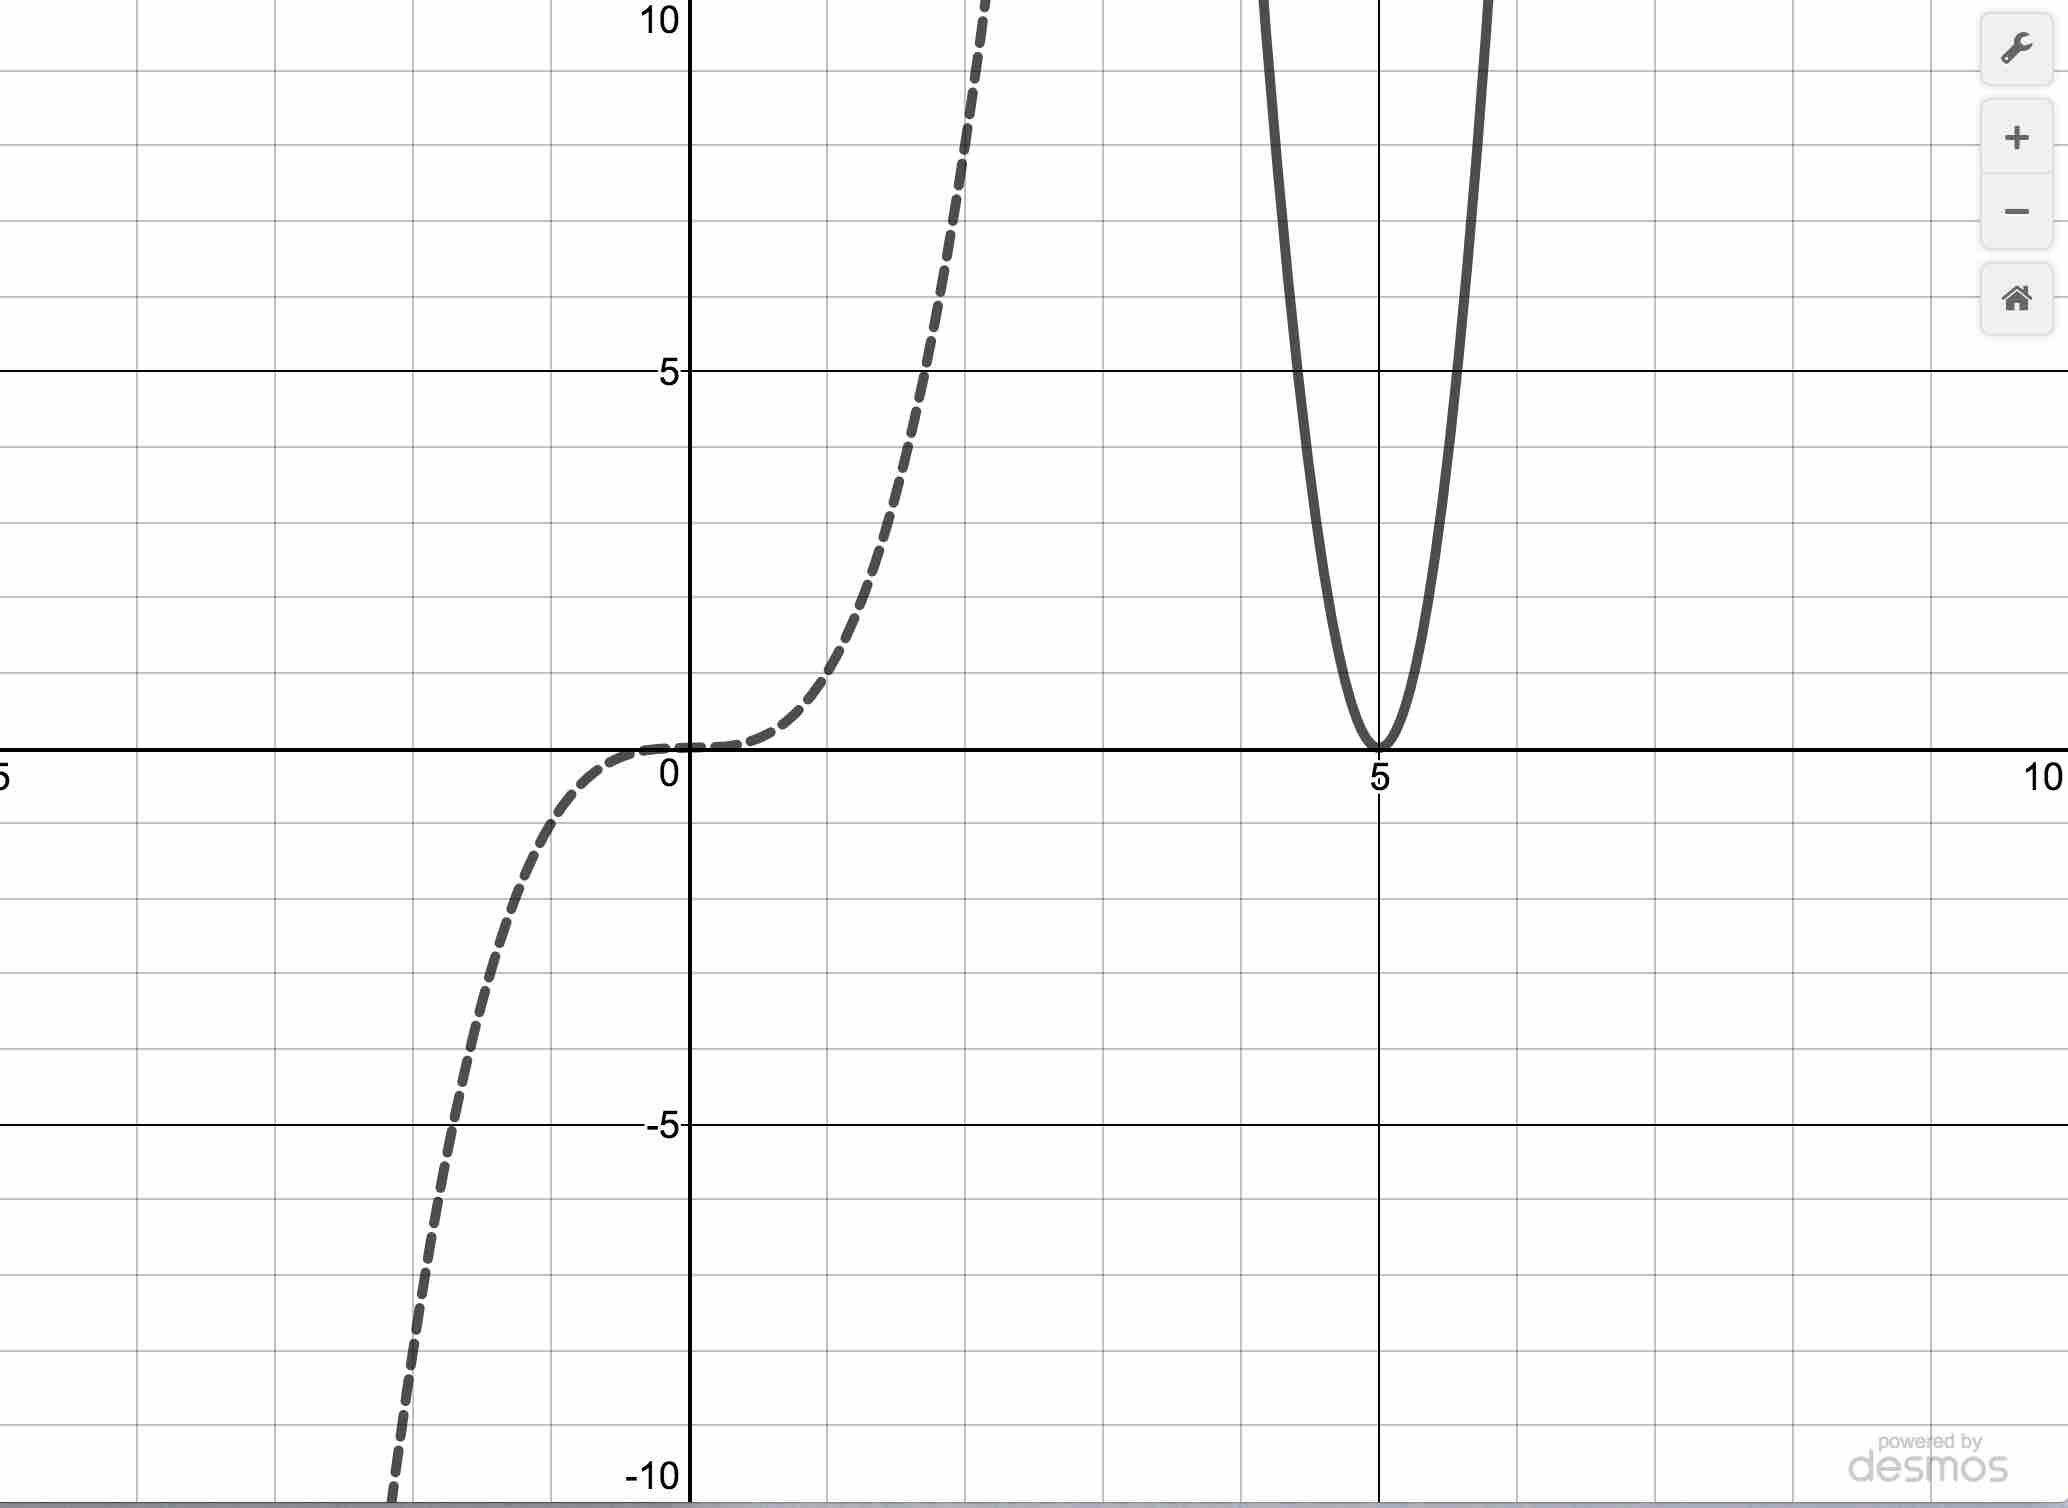
\includegraphics[height=2in]{./GraphsofPolynomialsGraphics/PolyEBEx1a.jpg}   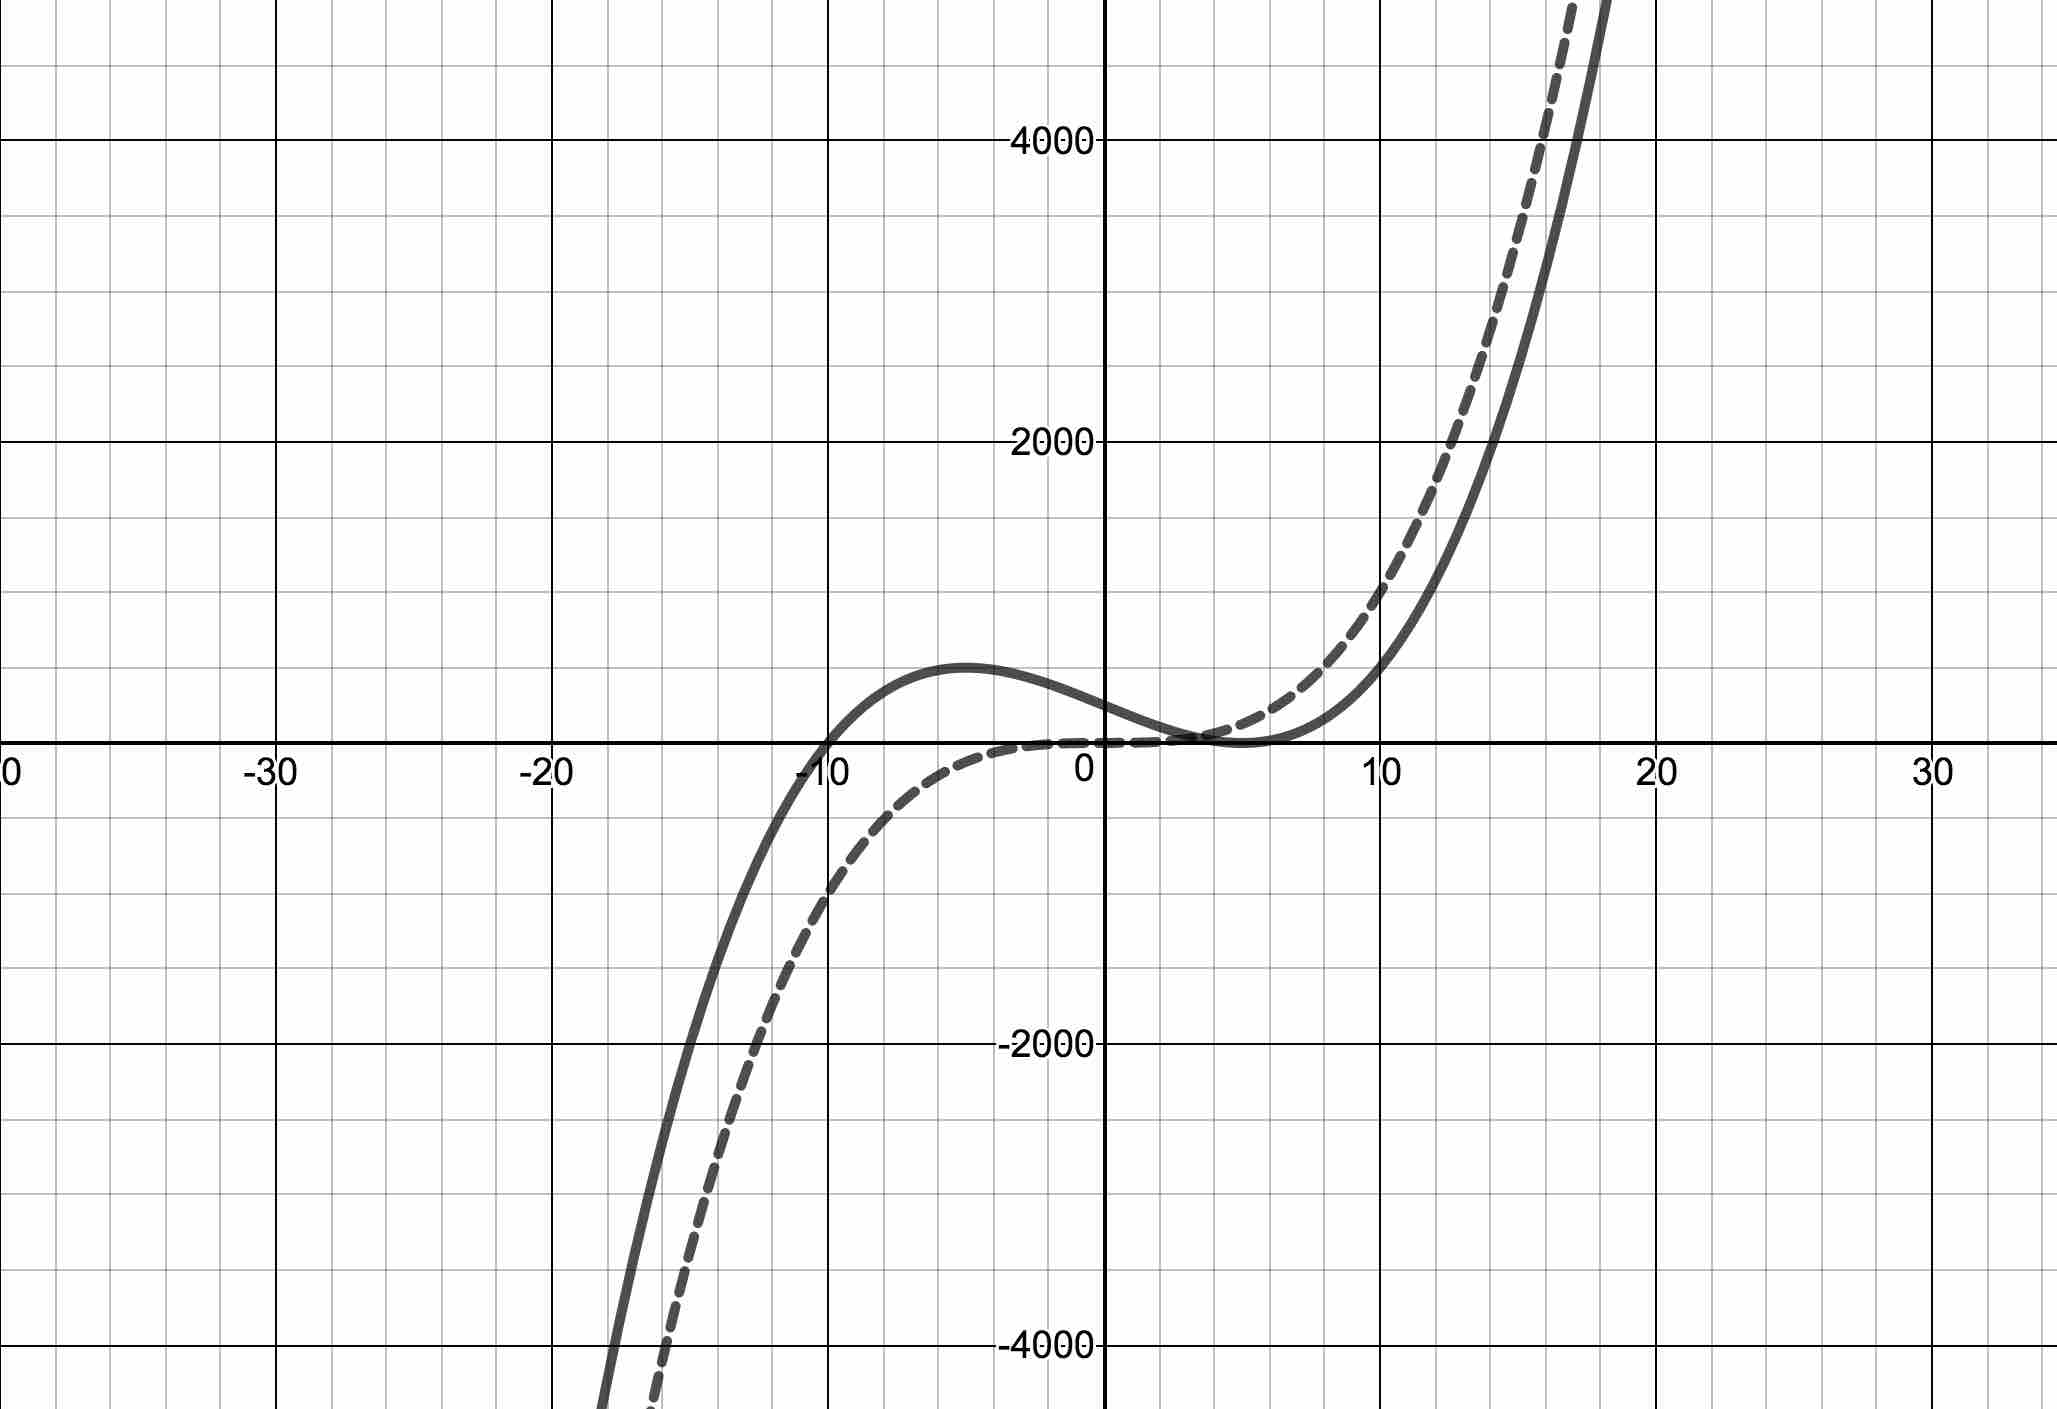
\includegraphics[height=2in]{./GraphsofPolynomialsGraphics/PolyEBEx1b.jpg} 


\end{multicols}


This observation is borne out numerically as well.  Based on the table below, as $x \rightarrow \pm \infty$, it certainly appears as if $f(x) \approx g(x)$.  One way to think about what is happening numerically is that the leading term $x^3$ \textit{dominates} the lower order terms  $-75x$ and $250$ as $x \rightarrow \pm \infty$.  In other words, $x^3$ grows so much faster than $-75 x$ and $250$ that these `lower order terms' don't contribute anything of significance to the $x^3$ so $f(x) \approx x^3$.  Another way to see this is to rewrite $f(x)$ as\footnote{Since we are considering  $x \rightarrow \pm \infty$, we are not concerned with $x$ even being close to $0$, so these fractions will all be defined.}   \[f(x) = x^3  - 75x + 250 = x^3 \left(1 -  \frac{75}{x^2} + \frac{250}{x^3} \right).\]   As $x \rightarrow \pm \infty$, both $\frac{75}{x^2}$ and $\frac{250}{x^3}$ have constant numerators but denominators that are becoming unbounded.  As such, both  $\frac{75}{x^2}$ and $\frac{250}{x^3} \rightarrow 0$.  Therefore, as $x \rightarrow \pm \infty$, \[ f(x) = x^3 - 75x+250  = x^3 \left(1 -  \frac{75}{x^2} + \frac{250}{x^3} \right) \approx x^3 (1 + 0 + 0) = x^3. \]

\[ \begin{array}{|r||c|c|c|c|c|c|}  \hline

 x &  f(x) = x^3 -75x+250 &  x^3 & -75 x & 250 & \frac{75}{x^2} &  \frac{250}{x^3}  \\ \hline
 -1000 & \approx -1 \times 10^9  &   -1 \times 10^9 &75000  & 250 & 7.5 \times 10^{-5} & -2.5 \times 10^{-7} \\  \hline
 -100 & \approx -9.9 \times 10^5 & -1 \times 10^6 & 7500  & 250 & 0.0075 & -2.5 \times 10^{-4} \\  \hline
 -10 & 0  & -1000  & 750 & 250  & 0.75   & -0.25\\  \hline
 10 & 500 &  1000 &  -750 & 250   & 0.75  &  0.25   \\ \hline
 100 &\approx 9.9 \times 10^5  & 1 \times 10^6 &   -7500  & 250 &  0.0075 &   2.5 \times 10^{-4} \\ \hline
 1000 & \approx 1 \times 10^9 & 1 \times 10^9  & -75000 & 250 & 7.5 \times 10^{-5} & 2.5 \times 10^{-7} \\  \hline

\end{array} \]


Next, consider  $g(x) = -0.01x^4 + 5x^2$.  Following the logic of the above example, we would expect the end behavior of $y=g(x)$ to mimic that of $y = -0.01 x^4$.  When we graph $y = g(x)$ (solid line) on the same set of axes as $y = -0.01x^4$ (dashed line), a view near the origin seems to suggest the exact opposite.  However, zooming out reveals that the two graphs do share the same end behavior.\footnote{Or at least they appear to within the limits of the technology.}


\begin{multicols}{2}

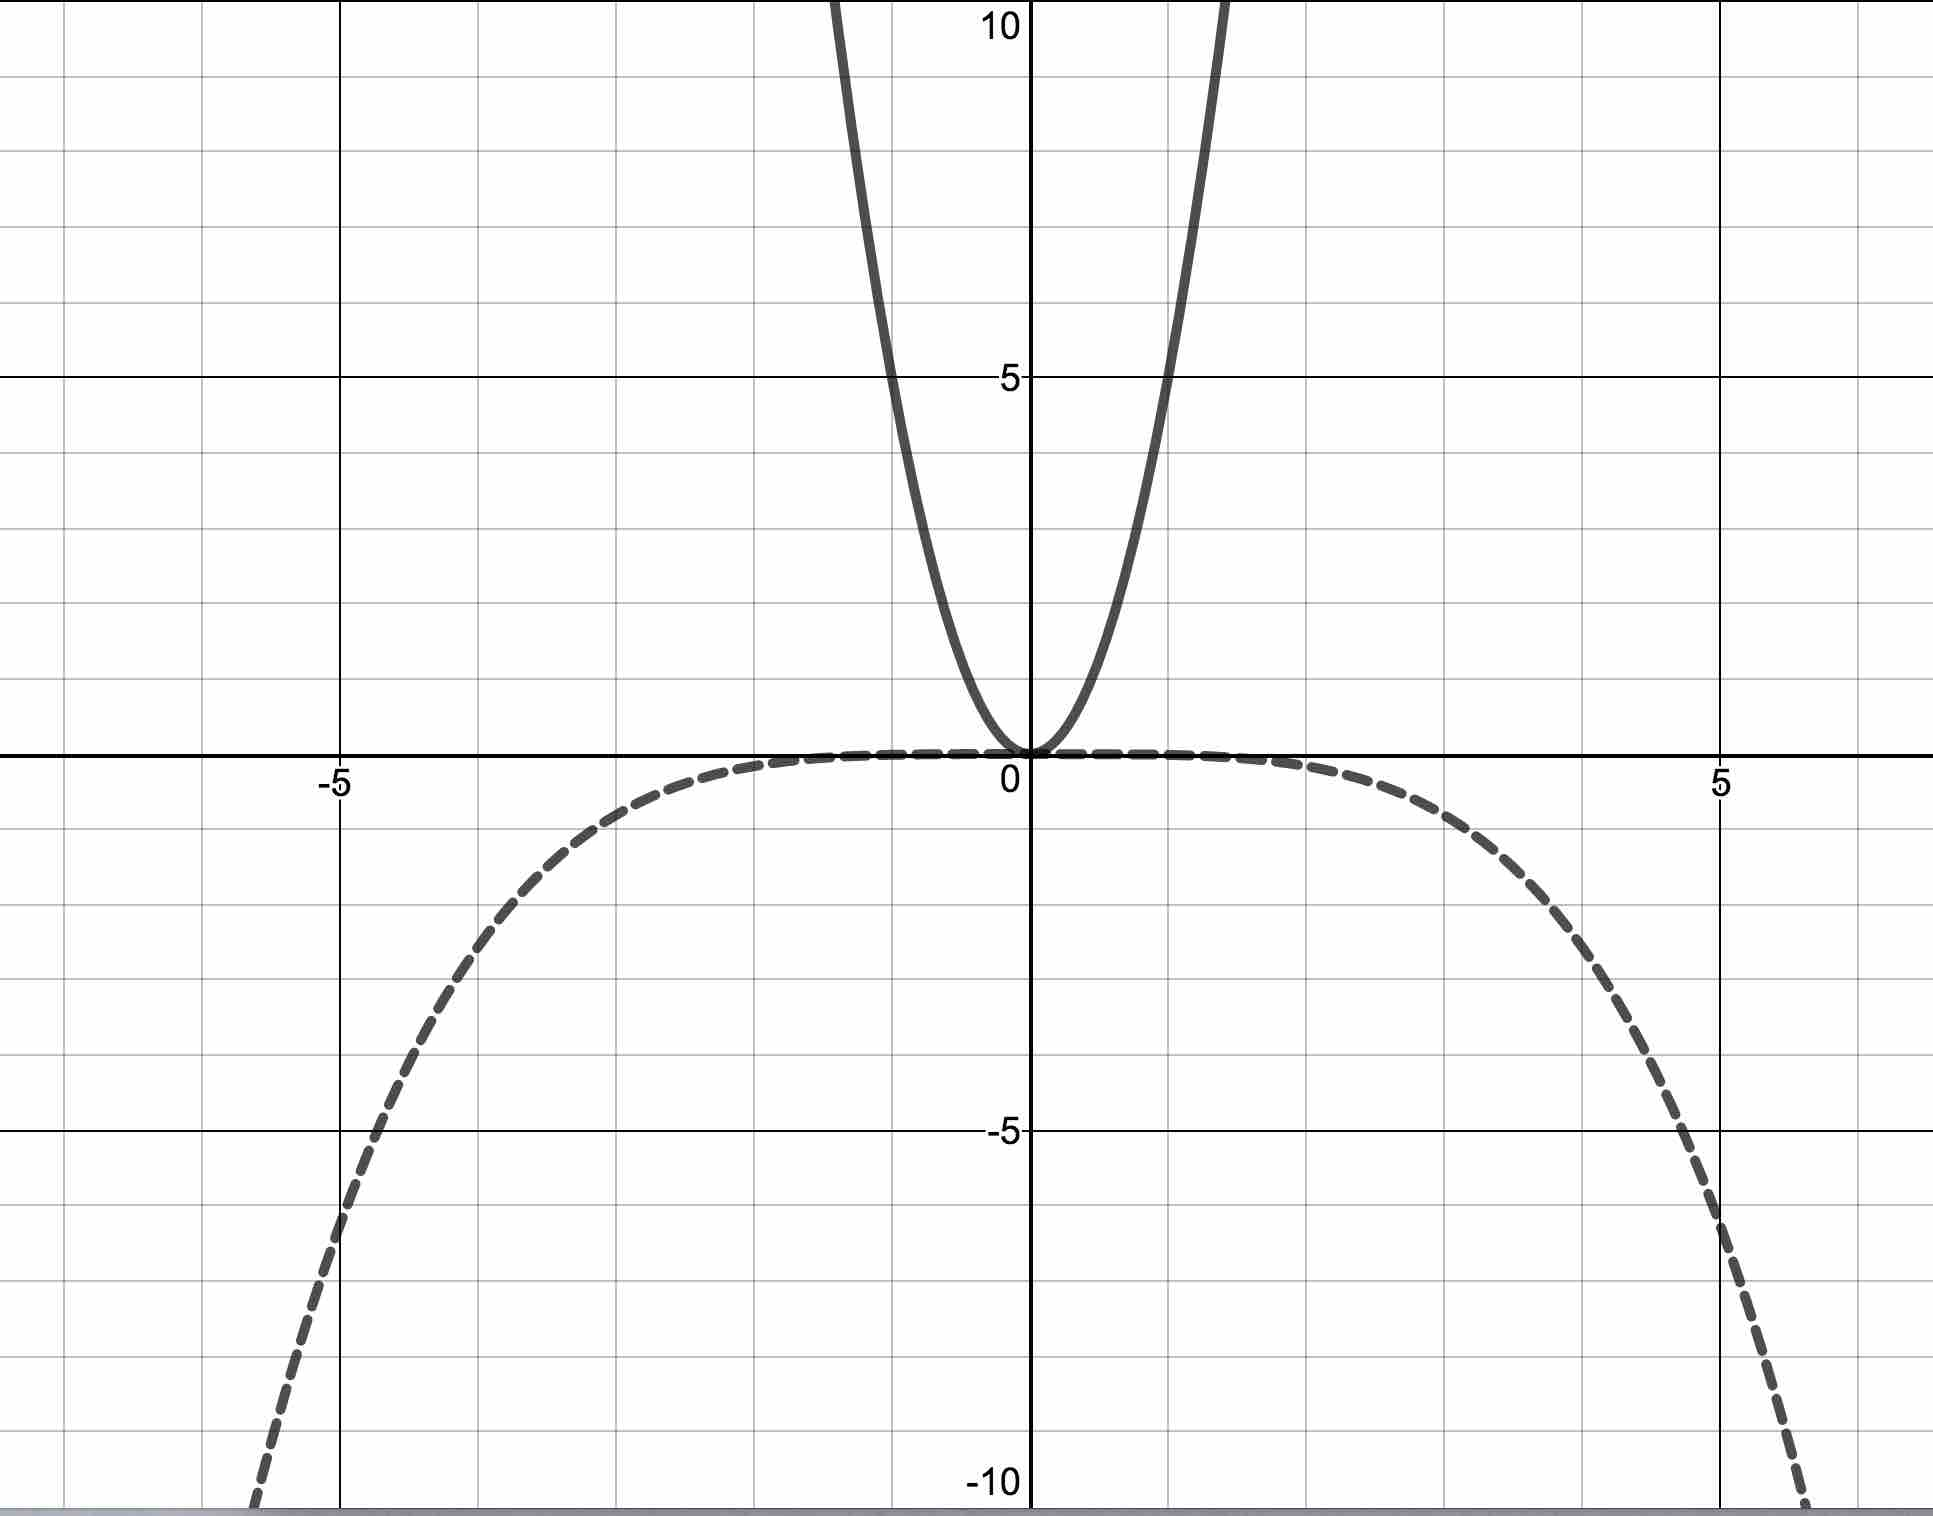
\includegraphics[height=2in]{./GraphsofPolynomialsGraphics/PolyEBEx2a.jpg}  \hspace{.5in} 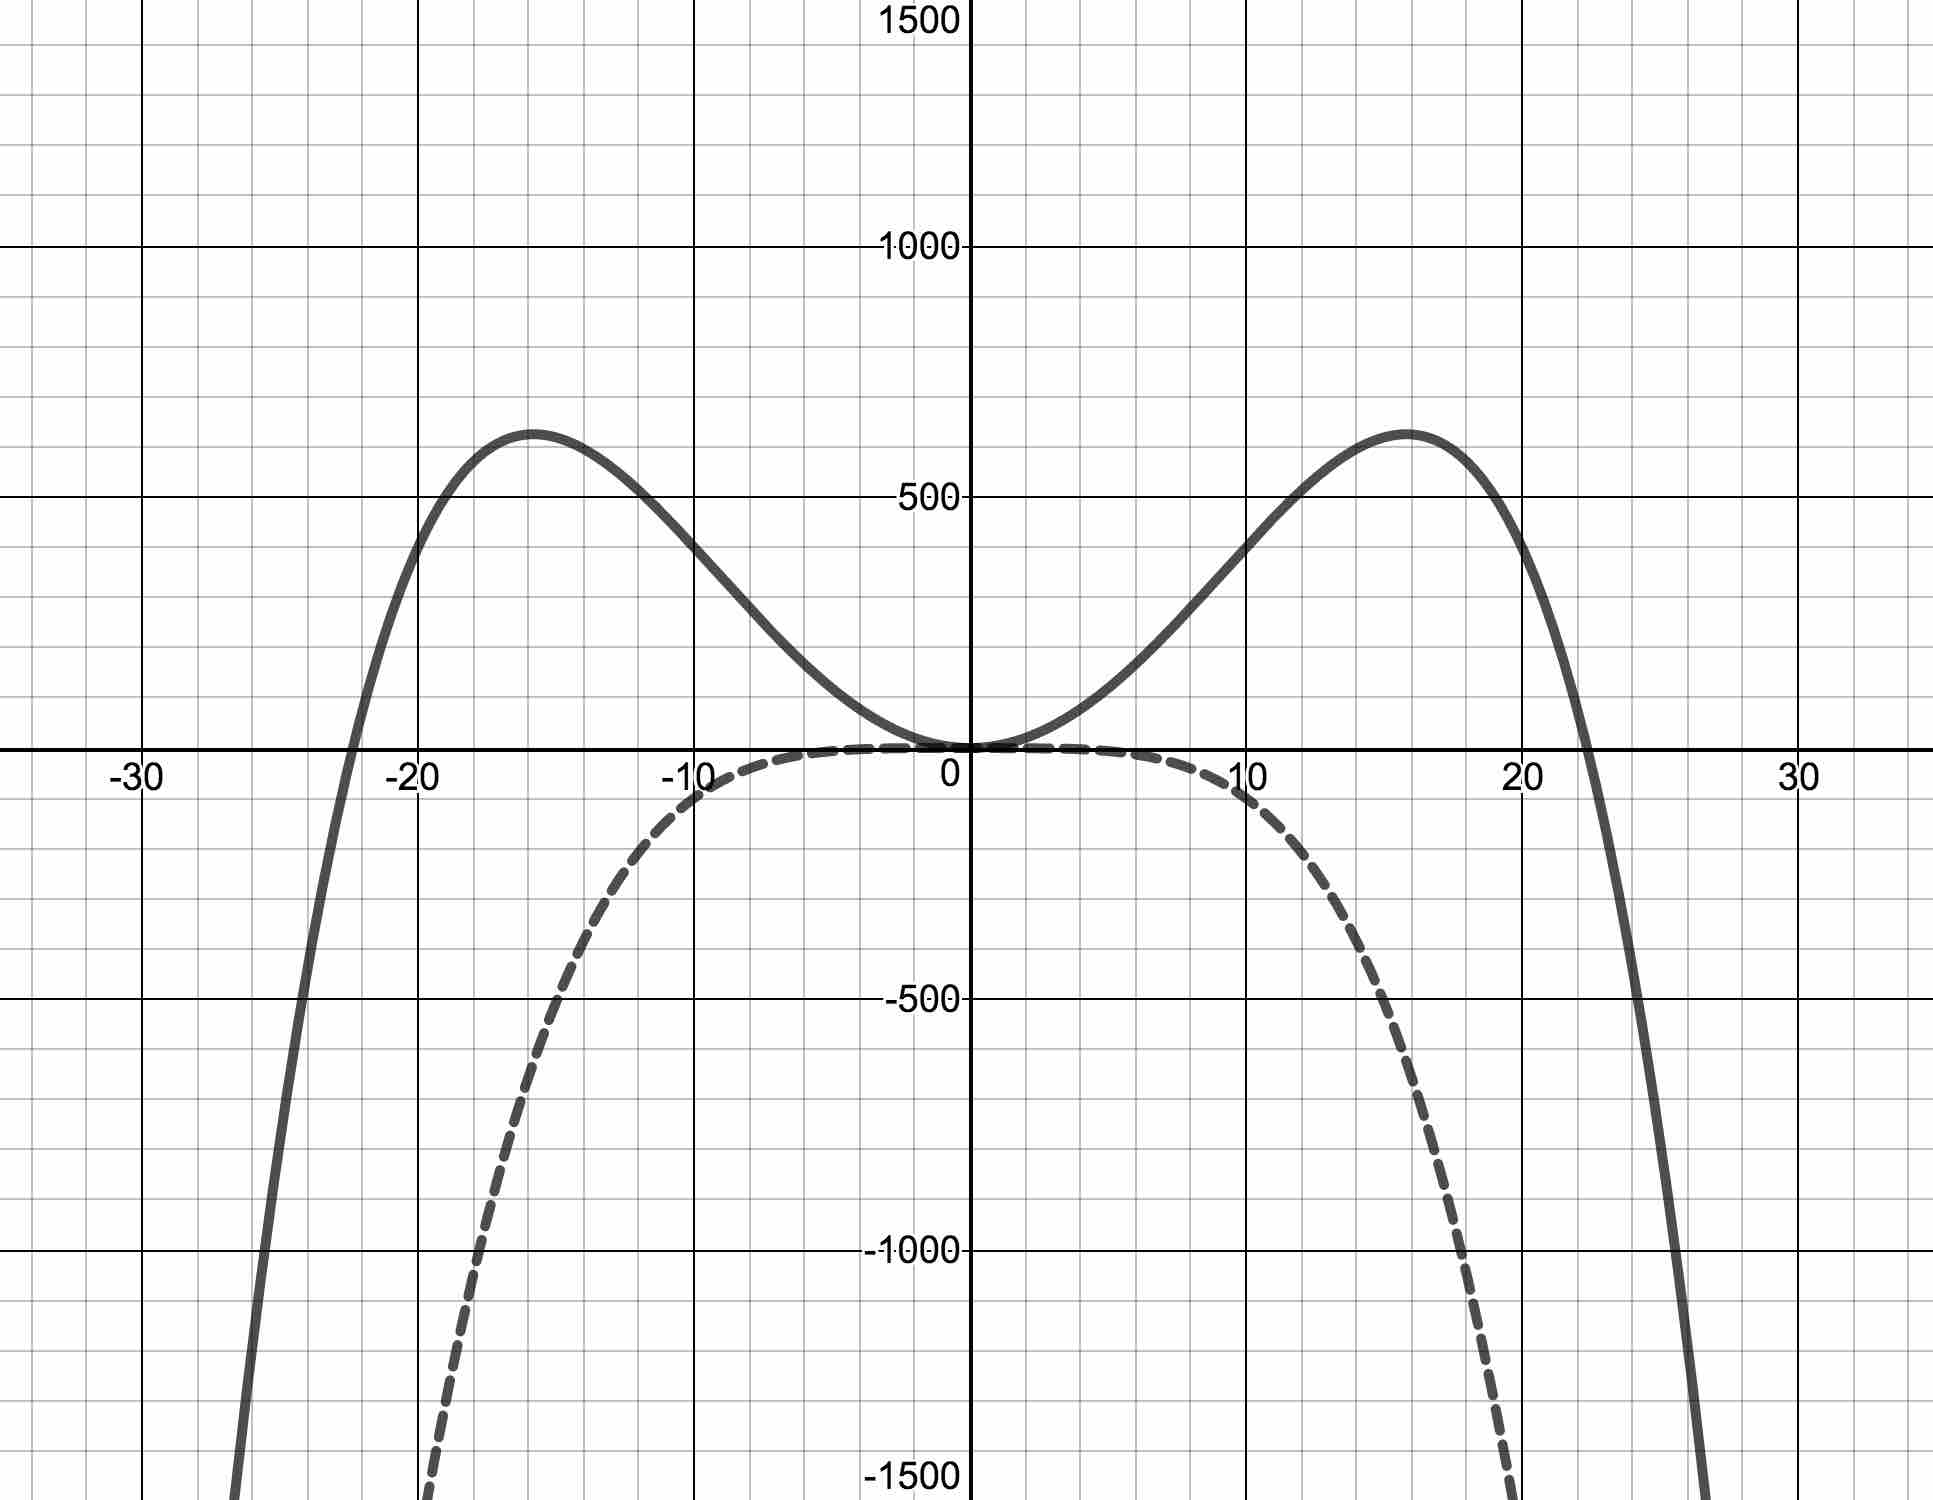
\includegraphics[height=2in]{./GraphsofPolynomialsGraphics/PolyEBEx2b.jpg} 


\end{multicols}

Algebraically, for $x \rightarrow \pm \infty$, even with the small coefficient of $-0.01$, $-0.01x^4$ dominates the $5x^2$ term so $g(x) \approx -0.01 x^4$.  More precisely, \[g(x) = -0.01x^4+5x^2 = x^4 \left(-0.01 + \frac{5}{x^2} \right) \approx x^4(-0.01 + 0)= -0.01x^4. \]

The results of these last two examples generalize below in Theorem \ref{EBPolynomials}.  


\colorbox{ResultColor}{\bbm

\begin{thm} \label{EBPolynomials}\index{end behavior ! polynomial}\textbf{End Behavior for Polynomial Functions:} 

The end behavior of  polynomial function $f(x) = a_{n} x^{n} + a_{n-\mbox{\tiny$1$}} x^{n-\mbox{\tiny$1$}} + \ldots + a_{\mbox{\tiny $2$}} x^{\mbox{\tiny $2$}} + a_{\mbox{\tiny $1$}} x + a_{\mbox{\tiny $0$}}$ with $a_{n} \neq 0$ matches the end behavior of $y = a_{n} x^{n}$.  

That is, the end behavior of a polynomial function is determined by its leading term.
\end{thm}

\ebm}

\medskip


We argue Theorem \ref{EBPolynomials} using an argument similar to ones used above.  As $x \rightarrow \pm \infty$, 

\[ f(x) =  x^{n} \left( a_{n} +\dfrac{a_{n-\mbox{\tiny$1$}}}{x}+ \ldots + \dfrac{a_{\mbox{\tiny$2$}}}{x^{n-2}} + \dfrac{a_{\mbox{\tiny$1$}}}{x^{n-1}}+\dfrac{a_{\mbox{\tiny$0$}}}{x^{n}}\right) \approx x^n( a_{n} + 0 +\ldots 0) = a_{n} x^n \]

If this argument looks a little fuzzy, it should.  In Calculus, we have the tools necessary to more explicitly state what we mean by $\approx 0$.  For now, we'll rely on number sense and algebraic intuition.\footnote{Both of which, by the way, can lead one astray, so we must proceed cautiously.}


Now that we know how to determine the end behavior of polynomial functions,  it's time to investigate what happens `in between' the ends.  First and foremost, polynomial functions are  \index{continuous}\index{function ! continuous}\textbf{continuous}.  Recall from Section \ref{QuadraticFunctions} that, informally, graphs of continuous functions have no `breaks' or `holes' in them.\footnote{Again, the formal definition of `continuity' and properties of continuous functions are discussed in Calculus.}   Since monomial functions are continuous (as far as we can tell) and polynomials are sums of monomial functions, it turns out that polynomial functions are continuous as well.   Moreover, the graphs of monomial functions, hence polynomial functions, are  \index{smooth}\index{function ! smooth}\textbf{smooth}.  Once again, `smoothness' is a concept defined precisely in Calculus, but for us,  functions have no `corners' or `sharp turns'.  Below we find the graph of a function which is neither smooth nor continuous, and to its right we have a graph of a polynomial, for comparison.  The function whose graph appears on the left fails to be continuous where it has a `break' or `hole' in the graph;  everywhere else, the function is continuous.  The function is continuous at the `corner' and the `cusp', but we consider these `sharp turns', so these are places where the function fails to be smooth.  Apart from these four places, the function is smooth and continuous.  Polynomial functions are smooth and continuous everywhere, as exhibited in the graph on the right.   The notion of smoothness is what tells us graphically that, for example, $f(x) = |x|$, whose graph is the characteristic `$\vee$' shape, cannot be a polynomial function, even though it is a piecewise-defined function comprised of polynomial functions.   Knowing polynomial functions are continuous and smooth gives us an idea of how to `connect the dots' when sketching the graph from points that we're able to find analytically such as intercepts.

\phantomsection
\label{cusppicture} 

\medskip

\begin{center}


\begin{tabular}{cc}

\begin{mfpic}[15]{-5}{5}{-2}{5}
\penwd{1.25pt}
\arrow \polyline{(-3,2),(-5,4)}
\arrow \function{-3,-1.5,0.1}{1-(2/(x+1))}
\dashed \polyline{(-1,0),(-1,5)}
\arrow \parafcn{-1,1.75,0.1}{(t**3,(t**2)+1)} 
\point[4pt]{(-1,2)}
\pointfillfalse
\point[4pt]{(3.375,3.25)}
\tlabel[cc](-3,1.5){\scriptsize  `corner'}
\tlabel[cc](-1,-0.5){\scriptsize `break'}
\tlabel[cc](0,0.5){\scriptsize `cusp'}
\tlabel[cc](3.375,2.5){\scriptsize `hole'}
\tcaption{\scriptsize Pathologies not found on graphs of polynomials functions.}
\end{mfpic}

\hspace{0.75in} &

\begin{mfpic}[15][7.5]{-5}{5}{-10}{10}
\penwd{1.25pt}
\arrow \reverse \arrow \function{-3,3.5,0.1}{0.5*x*(x+2)*(x-3)}
\tcaption{\scriptsize   The graph of a polynomial function.}
\end{mfpic}

\end{tabular}

\end{center}



Speaking of intercepts,  we next focus our attention on the behavior of the graphs of polynomial functions near their zeros.    Recall a zero $c$ of a function $f$ is a solution to $f(x) = 0$.  Geometrically, the zeros of a function are the $x$-coordinates of the $x$-intercepts of the graph of $y = f(x)$.    Consider the polynomial function $f(x) = x^3 (x-2)^2 (x+1)$. To find the zeros of $f$, we set $f(x) =  x^3 (x-2)^2 (x+1) = 0$.  Since the expression $f(x)$ is already factored, we set each factor equal to zero.\footnote{in accordance with the Zero Product Property of the Real Numbers - see Section \ref{AppRealNumberArithmetic}.}  Solving $x^3 = 0$ gives $x = 0$, $(x-2)^2 = 0$ gives $x = 2$, and $x+1 = 0$ gives $x = -1$.  Hence, our zeros are $x = -1$, $x = 0$, and $x = 2$.  Below, we graph $y = f(x)$ and observe the $x$-intercepts $(-1,0)$, $(0,0)$ and $(2,0)$.  We first note that the graph \textit{crosses} through the $x$-axis at $(-1,0)$ and $(0,0)$, but the graph \textit{touches} and \textit{rebounds} at $(2,0)$.  Moreover, at $(-1,0)$, the graph crosses through the axis is a fairly `linear' fashion whereas there is a substantial amount of `flattening' going on near $(0,0)$.  Or aim is to explain these observations and generalize them.

\begin{center}

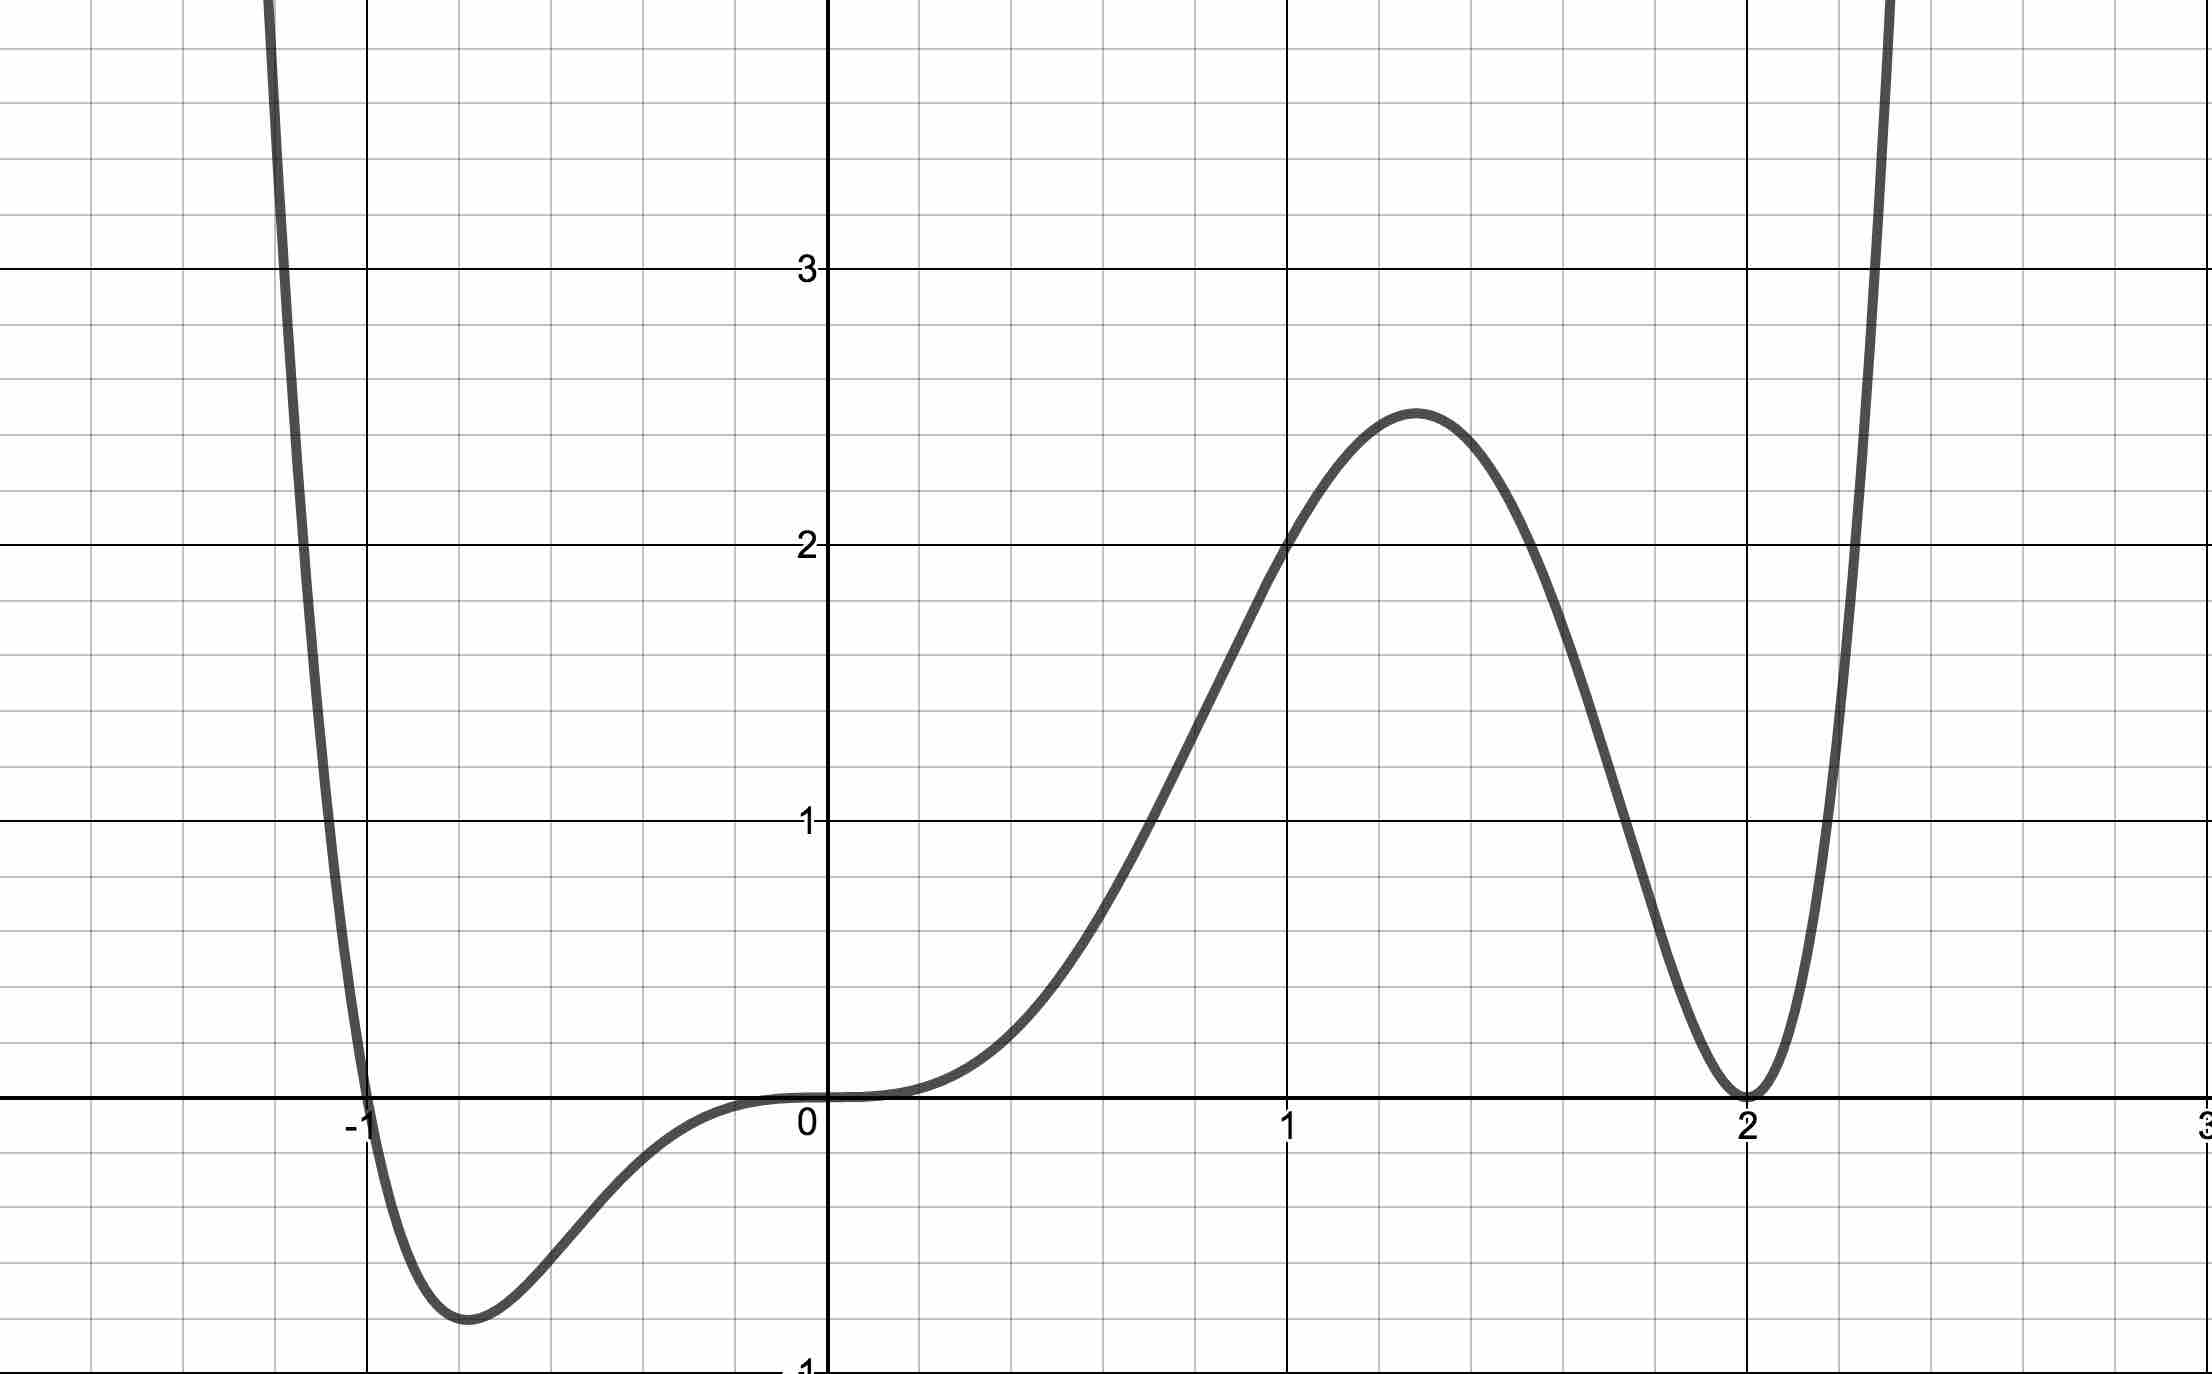
\includegraphics[height=3in]{./GraphsofPolynomialsGraphics/PolyZeroEx01.jpg} 

\end{center}

First, let's look at what's happening with the formula  $f(x) =  x^3 (x-2)^2 (x+1)$  when  $x  \approx  -1$.   We know the $x$-intercept at $(-1,0)$ is due to the presence of the $(x+1)$ factor in the expression for $f(x)$.  So, in this sense, the factor $(x+1)$ is determining a major piece of the behavior of the graph near $x = -1$.   For that reason, we focus instead on the other two factors to see what contribution they make. We find when $x \approx -1$,  $x^3  \approx  (-1)^3 = -1$ and $(x-2)^2 \approx (-1-2)^2 = 9$.  Hence, $f(x) = x^3 (x-3)^2 (x+1) \approx (-1)^3 (-1-2)^2 (x+1) = -9(x+1)$.  Below on the left is a graph of $y = f(x)$ (the solid line) and the graph of $y = -9(x+1)$ (the dashed line.)  Sure enough, these graphs approximate one another near $x = -1$. 

Likewise, let's look near $x = 0$.  The $x$-intercept $(0,0)$ is due to the $x^3$ term.  For $x \approx 0$, $(x-2)^2 \approx (0-2)^2 = 4$ and $(x+1) \approx (0+1) = 1$, so $f(x) =  x^3 (x-3)^2 (x+1) \approx x^3 (-2)^2(1) = 4x^3$.  Below in the center picture, we have the graph of $y = f(x)$ (again, the solid line) and $y = 4x^3$ (the dashed line) near $x=0$.  Once again, the graphs verify our analysis.

Last, but not least, we analyze $f$ near $x = 2$.  Here, the intercept $(2,0)$ is due to the $(x-2)^2$ factor, so we look at the $x^3$ and $(x+1)$ factors.  If $x \approx 2$, $x^3 \approx (2)^3 = 8$ and $(x+1) \approx (2+1) = 3$.  Hence,  $f(x) =  x^3 (x-3)^2 (x+1) \approx (2)^3 (x-2)^2 (2+1) = 24(x-2)^2$.  Sure enough, as evidenced below on the right, the graphs of $y = f(x)$ and $y = 24(x-2)^2$.


\begin{tabular}{m{2in}m{2in}m{2in}}

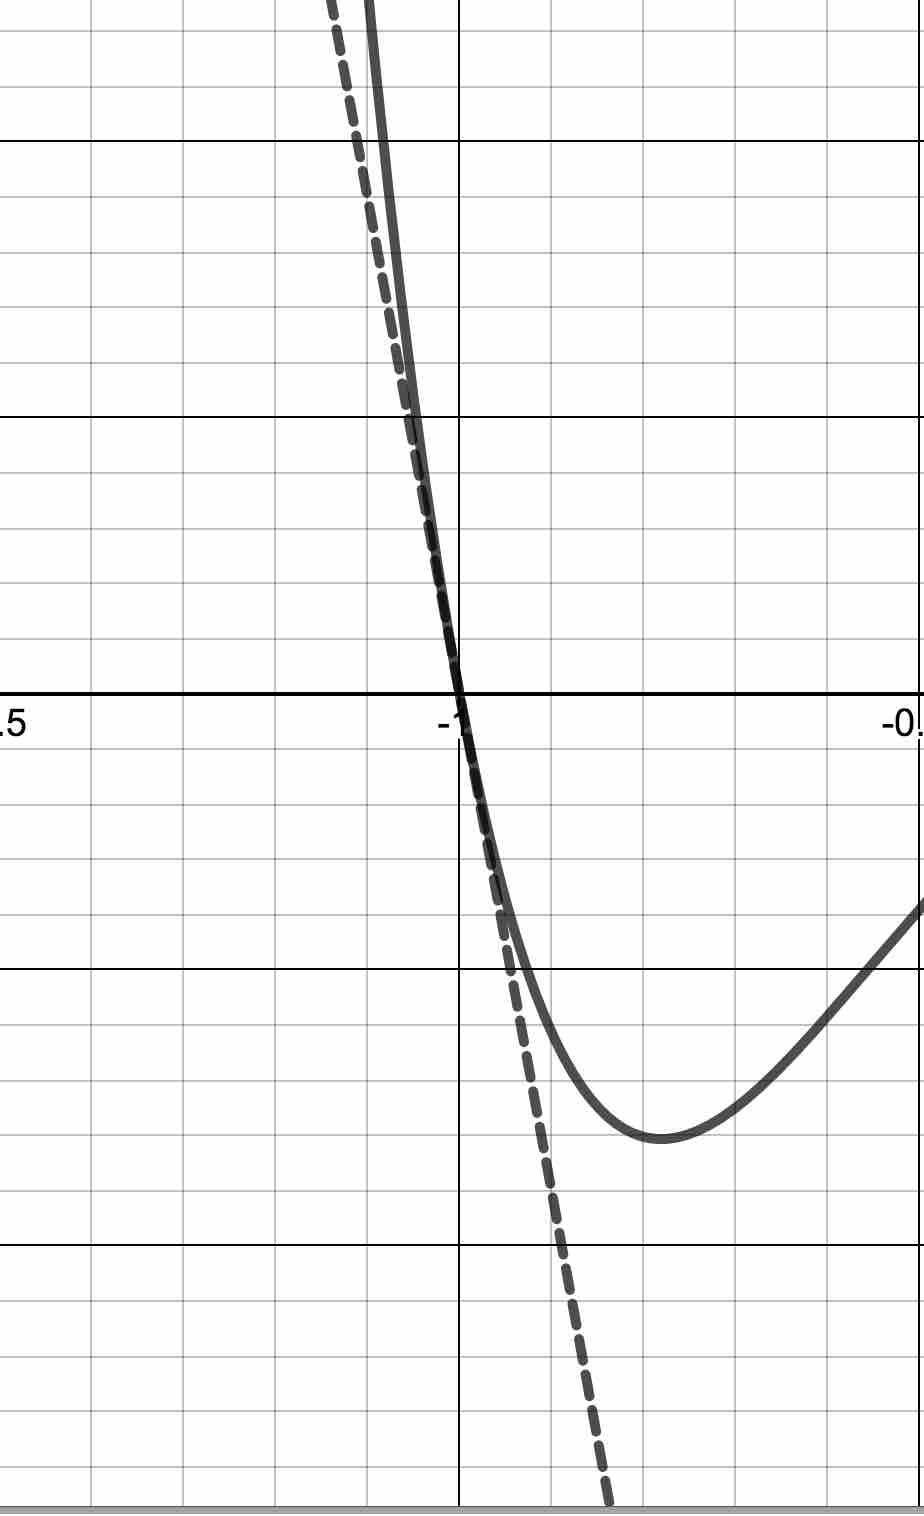
\includegraphics[height=2.in, width=2.in]{./GraphsofPolynomialsGraphics/PolyZeroEx02.jpg} 
&

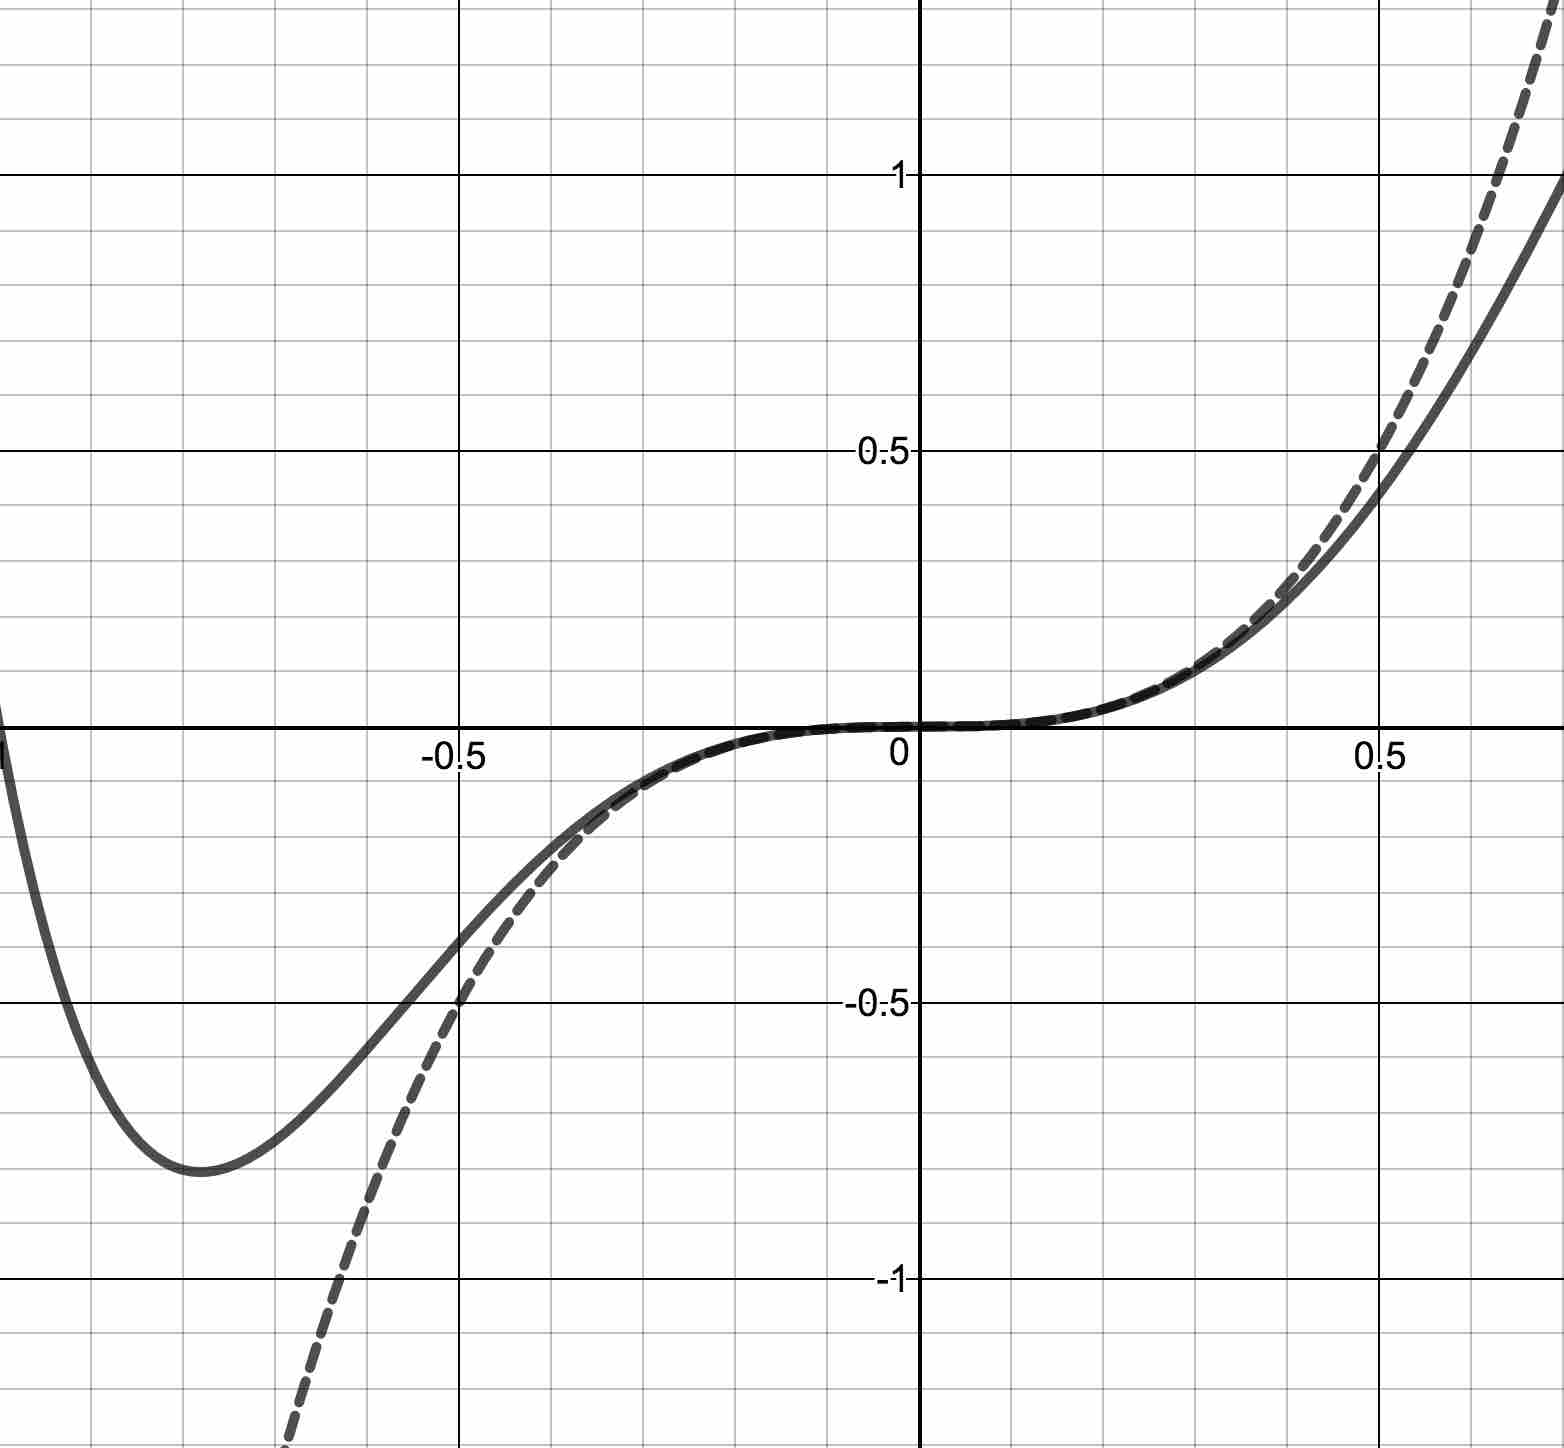
\includegraphics[height=2.in, width=2.in]{./GraphsofPolynomialsGraphics/PolyZeroEx03.jpg} 

&

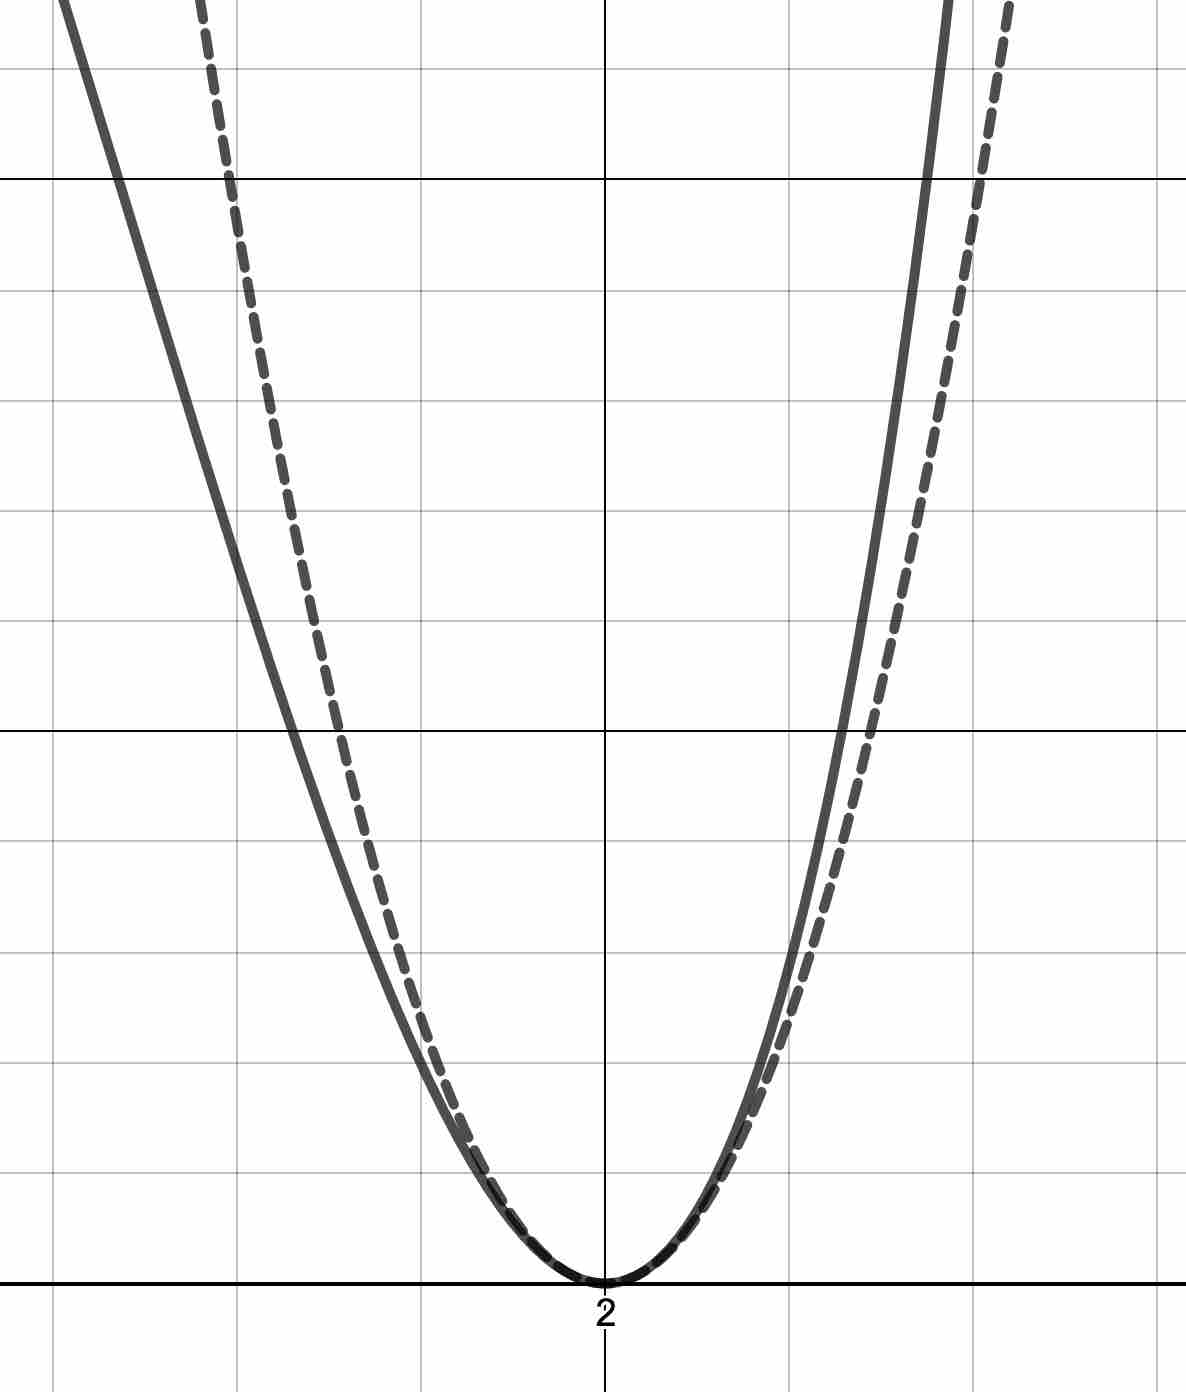
\includegraphics[height=2.in, width=2.in]{./GraphsofPolynomialsGraphics/PolyZeroEx04.jpg}  \\

$y = f(x)$ and $y = -9(x+1)$

&

$y = f(x)$ and $y = 4x^3$ 

&

$y = f(x)$ and $y=24(x-2)^2$ \\

\end{tabular}

We generalize our observations in Theorem \ref{polynomialbehaviornearzeros} below. Like many things we've seen in this text, a more precise statement and proof can be found in a course on Calculus.

\colorbox{ResultColor}{\bbm

\begin{thm}  \label{polynomialbehaviornearzeros}  Suppose $f$ is a polynomial function and $f(x) = (x-c)^m q(x)$ where $m \in \mathbb{N}$ and $q(c) \neq 0$.  Then the the graph of $y = f(x)$ near $(c,0)$ resembles that of $y = q(c) (x-c)^m$.


\end{thm}

\ebm}

Let's see how Theorem \ref{polynomialbehaviornearzeros}  applies to our findings regarding $f(x) =  x^3 (x-2)^2 (x+1)$. For $c = -1$, $(x-c) = (x-(-1)) = (x+1)$.  We  rewrite $f(x) =  x^3 (x-2)^2 (x+1) = (x-(-1))^1 \left[x^3(x-2)^2\right]$ and identify $m=1$ and $q(x) = x^3 (x-2)^2$.  We find $q(c) = q(-1) = (-1)^3(-1-2)^2 = -9$ so  Theorem \ref{polynomialbehaviornearzeros} says that near $(-1,0)$, the graph of $y=f(x)$ resembles $y = q(-1)(x-(-1))^1 = -9(x+1)$.  For $c=0$, $(x-c) = (x-0) = x$ and we can rewrite $f(x) =  x^3 (x-2)^2 (x+1) = (x-0)^3 \left[(x-2)^2 (x+1)\right]$.  We identify $m=3$ and $q(x) = (x-2)^2(x+1)$.  In this case $q(c) = q(0) = (0-2)^2(0+1) = 4$, so  Theorem \ref{polynomialbehaviornearzeros} guarantees the graph  of $y = f(x)$ near $x=0$ resembles  $y = q(0)(x-0)^3 = 4x^3$.  Lastly, for $c = 2$, we see $f(x) = (x-2)^2 \left[x^3 (x+1)\right]$ and we identify $m = 2$ and $q(x) = x^3(x+1)$.  We find $q(2) = 2^3 (2+1)= 24$, so  Theorem \ref{polynomialbehaviornearzeros}  guarantees the graph of $y = f(x)$ resembles $y = 24(x-2)^2$ near $x=2$.

As we already mentioned,  the formal statement and proof of Theorem \ref{polynomialbehaviornearzeros} require Calculus.  For now, we can understand the theorem as follows.   If we factor a polynomial function as $f(x) = (x-c)^m q(x)$ where $m \geq 1$,   then $x=c$ is a zero of $f$, since $f(c) = (c-c)^m q(c) = 0 \cdot q(c) = 0$.  The stipulation that $q(c) \neq 0$ means that we have essentially factored the expression $f(x) = (x-c)^m q(x) = (\text{going to $0$}) \cdot (\text{not going to $0$})$.   Thinking back to Theorem \ref{linearmononialgraphs}, the graph $y = q(c) (x-c)^m$ has an $x$-intercept at $(c,0)$, a basic overall shape determined by the exponent $m$, and end behavior determined by the sign of $q(c)$.   The fact that \textit{if} $x=c$ is a zero \textit{then} we are guaranteed we can factor $f(x) = (x-c)^m q(x)$ were $q(c) \neq 0$ and, moreover, such a factorization is unique (so that there's only one value of $m$ possible for each zero) is a consequence of two theorems, Theorem \ref{polydivthm} and The Factor Theorem, Theorem \ref{factorthm} which we'll review in Section \ref{Polydivision}.  For now, we assume such a factorization is unique in order to define the following.

\colorbox{ResultColor}{\bbm

\begin{defn} \label{multiplicity} Suppose $f$ is a polynomial function and $m \in \mathbb{N}$. If $f(x) = (x-c)^m q(x)$ where $q(c) \neq 0$, we say  $x=c$ is a zero of \index{polynomial function ! zero ! multiplicity}\index{multiplicity ! of a zero}\index{zero ! multiplicity of}\textbf{multiplicity} $m$.

\end{defn}

\ebm}

So, for $f(x) =  x^3 (x-2)^2 (x+1) = (x-0)^3(x-2)^2(x-(-1))^1$, $x=0$ is a zero of multiplicity $3$, $x=2$ is a zero of multiplicity $2$, and $x =-1$ is a zero of multiplicity $1$.  Theorems   \ref{EBPolynomials}  and \ref{polynomialbehaviornearzeros} give us the following:


\colorbox{ResultColor}{\bbm

\begin{thm} \label{roleofmultiplicity} \textbf{The Role of Multiplicity:}  Suppose $f$ is a polynomial function  and $x=c$ is a zero of multiplicity $m$.  \index{multiplicity ! effect on the graph of a polynomial}

\begin{itemize}

\item  If $m$ is even, the graph of $y=f(x)$ touches and rebounds from the $x$-axis at $(c,0)$.

\item  If $m$ is odd, the graph of $y=f(x)$ crosses through the $x$-axis at $(c,0)$.

\end{itemize}

\end{thm}

\ebm}


Our next example showcases how all of the above theory can assist in sketching relatively good graphs of polynomial functions without the assistance of technology.

\begin{ex} \label{graphfromtheory}   Let $p(x) = (2x-1)(x+1)(1-x^4)$.

\begin{enumerate}

\item Find all real zeros of $p$ and state their multiplicities.

\item  Describe the behavior of the graph of $y = p(x)$ near each of the $x$-intercepts.

\item  Determine the end behavior  and $y$-intercept of the graph of  $y = p(x)$.

\item  Sketch $y = p(x)$ and check your answer using a graphing utility.

\end{enumerate}

{\bf Solution.}

\begin{enumerate}

\item  To find the zeros of $p$, we set  $p(x) =  (2x-1)(x+1)(1-x^4) = 0$.  Since the expression $p(x)$ is already (partially) factored, we set each factor equal to $0$ and solve.  From $(2x-1) =0$, we get $x=\frac{1}{2}$; from $(x+1) = 0$ we get  $x = -1$; and from  solving $1-x^4 =0$ we get $x = \pm 1$.  Hence, the zeros are $x = -1$, $x = \frac{1}{2}$, and $x = 1$.  In order to determine the multiplicities, we need to factor $p(x)$ as so we can identify the $m$ and $q(x)$ as described in Definition \ref{multiplicity}.  The zero $x = -1$ corresponds to the factor $(x+1)$.  Notice, however, that writing $p(x) = (x+1)^1 \left[(2x-1)(1-x^4)\right]$ with $m = 1$ and $q(x) = (2x-1)(1-x^4)$ does \textit{not} satisfy Definition \ref{multiplicity} since here, $q(-1) = (2(-1)-1)(1-(-1)^4) = 0$.  Indeed, we can factor $(1-x^4) = (1-x^2)(1+x^2) = (1-x)(1+x)(x^2+1)$ so that \[p(x)= (2x-1)(x+1)(1-x^4)  = (2x-1)(x+1)(1-x)(1+x)(x^2+1) = (x+1)^2 \left[(2x-1)(1-x)(x^2+1) \right].\]
Identifying $q(x) = (2x-1)(1-x)(x^2+1)$, we find $q(-1) = (2(-1)-1)(1-(-1))((-1)^2+1) = -12 \neq 0$, which means the multiplicity of $x=-1$ is $m=2$.  

The zero $x = \frac{1}{2}$ came from the factor $(2x-1) = 2 (x-\frac{1}{2})$, so we have \[ p(x) =  (2x-1)(x+1)^2(1-x)(x^2+1)  = (x -\frac{1}{2})^{1} \left[2 (x+1)^2(1-x)(x^2+1) \right]. \] If we identify $q(x) = 2 (x+1)^2(1-x)(x^2+1)$, we find $q(\frac{1}{2}) = \frac{45}{16} \neq 0$ so multiplicity here is $m=1$.  

Last but not least, we turn our attention to our last zero, $x = 1$, which we obtained from solving $1-x^4=0$.  However, from $p(x) =  (2x-1)(x+1)^2(1-x)(x^2+1)$, we see the zero $x=1$ corresponds to the factor $(1-x) = -(x-1)$.  We have $p(x) = (x-1)^{1}\left[- (2x-1)(x+1)^2(x^2+1)\right]$.  Identifying $q(x) = - (2x-1)(x+1)^2(x^2+1)$, we see $q(1) = -8$, so the multiplicity $m = 1$ here as well.  


\item  From Theorem \ref{roleofmultiplicity}, since the multiplicities of $x = \frac{1}{2}$ and $x = 1$ are both \textit{odd}, we know the graph of $y = p(x)$ \textit{crosses} through the $x$-axis at $(\frac{1}{2}, 0)$ and $(1,0)$. More specifically, since the multiplicity for both of these zeros is $1$,  the graph will look locally linear at these points. More specifically, based on our calculations above, near $x = \frac{1}{2}$, the graph will resemble the increasing line $y =  \frac{45}{16} (x - \frac{1}{2})$, and near  $x = 1$, the graph will resemble the decreasing line $y = -8(x-1)$.    Since the multiplicity of $x = -1$ is \textit{even}, we know the graph of $y = p(x)$ \textit{touches} and  \textit{rebounds} at $(-1,0)$.   Since the multiplicity of $x=-1$ is $2$, it will look locally like a parabola.   More specifically, the graph near $x = -1$ will resemble $y = -12(x+1)^2$.

\item  Per Theorem \ref{EBPolynomials}, the end behavior of $y =p(x)$, matches the end behavior of its leading term.  As in Example \ref{degreandallthatexample}, we multiply the leading terms from each factor together to obtain the leading term for $p(x)$ :   $p(x) = (2x-1)(x+1)(1-x^4) = (2x)(x)(-x^4) + \ldots = -2x^6 + \ldots$.  Since the degree here, $6$, is even and the leading coefficient $-2 <0$, we know as $x \rightarrow \pm \infty$, $p(x) \rightarrow -\infty$.  To find the $y$-intercept, we find $p(0) = (2(0)-1)(0+1)(1-0^4) = -1$, hence, the $y$-intercept is $(0,-1)$.  

\item  From the end behavior, $x \rightarrow -\infty$, $p(x) \rightarrow -\infty$, we start the graph in Quadrant III and head towards $(-1,0)$. At $(-1,0)$, we `bounce' off of the $x$-axis and head towards the $y$-intercept, $(0,-1)$.  We then head towards $\left(\frac{1}{2}, 0 \right)$ and cross through the $x$-axis there.  Finally, we head back to the $x$-axis and cross through at $(1,0)$.  Owing to the end behavior $x \rightarrow \infty$, $p(x) \rightarrow -\infty$, we exit the picture in Quadrant IV.  Since polynomial functions are continuous and smooth, we have no holes or gaps in the graph, and all the `turns' are rounded (no abrupt turns or corners.)  We produce something resembling the graph below.

\begin{center}

\begin{mfpic}[40][20]{-2}{2}{-4}{2}
\axes
\scriptsize
\tlabel[cc](2, -0.5){$x$}
\tlabel[cc](0.25, 2){$y$}
\tlabel[cc](-1,0.5){$(-1,0)$}
\tlabel[cc](0.5,-1){$(0,-1)$}
\tlabel[cc](0.25, 0.5){$\left( \frac{1}{2},0 \right)$}
\tlabel[cc](1.25,0.5){$(1,0)$}
\normalsize
\penwd{1.25pt}
\arrow \reverse \arrow \function{-1.35,1.2,0.1}{(2*x-1)*(x+1)*(1-(x**4))}
\point[4pt]{(-1,0), (0.5,0), (1,0), (0,-1)}
\tcaption{\scriptsize $y=p(x)$}
\end{mfpic} 

\end{center}

\qed

\end{enumerate}


\end{ex}

A couple of remarks about Example \ref{graphfromtheory} are in order.  First, notice that the factor $(x^2+1)$ was more of a spectator in our discussion of the zeros of $p$. Indeed, if we set $x^2+1 = 0$, we have $x^2=-1$ which provides no \textit{real} solutions.\footnote{The solutions are $x = \pm i$ - see Section \ref{AppCmpNums}.}  That being said, the factor $x^2+1$ \textit{does} affect the shape of the graph (See Exercise \ref{comparegraphfromtheoryexample}.) Next, when connecting up the graph from $(-1,0)$ to $(0,-1)$ to $\left(\frac{1}{2}, 0 \right)$, there really is no way for us to know how low the graph goes, or where the lowest point is between $x = -1$ and $x = \frac{1}{2}$  unless we plot more points.  Likewise, we have no idea how high the graph gets between $x = \frac{1}{2}$ and $x = 1$.  While there are ways to determine these points analytically, more often than not, finding them requires Calculus.   Since these points do play an important role in many applications, we'll need to discuss them in this course and, when required, we'll  use technology to find them.   For that reason, we have the following definition:

\colorbox{ResultColor}{\bbm
\begin{defn}

\label{localmaxmindefn}

Suppose $f$ is a function with $f(a) = b$.

\begin{itemize}

\item  We say $f$ has a \textbf{local minimum} at the point $(a,b)$ if and only if there is an open interval $I$ containing $a$ for which $f(a) \leq f(x)$ for all $x$ in $I$.  The value $f(a) = b$ is called `a  local minimum value of $f$.' \index{local minimum ! formal definition of}

That is, $b$ is the minimum $f(x)$ value over an \textit{open interval}  containing $a$. 

 Graphically,  no points `near' a local minimum are lower than $(a,b)$. 

\item  We say $f$ has a \textbf{local maximum} at the point $(a,b)$ if and only if there is an open interval $I$ containing $a$ for which $f(a) \geq f(x)$ for all $x$ in $I$.  The value $f(a) = b$ is called `a  local maximum value of $f$.' \index{local maximum ! formal definition of}

That is, $b$ is the maximum $f(x)$ value over an \textit{open interval} containing $a$.  

Graphically, no points `near' a local maximum are higher than $(a,b)$. 

\end{itemize}

Taken together, the local maximums and local minimums of a function, if they exist,  are called the \textbf{local extrema} of the function. \index{local extrema ! formal definition of}



\end{defn}

\ebm}

Once again, the terminology used in Definition \ref{localmaxmindefn}  blurs the line between the function $f$ and its outputs, $f(x)$.  Also, some textbooks use the terms `relative' minimum and `relative' maximum instead of the adjective `local.'  Lastly, note  the definition of local extrema requires an \textit{open} interval exist in the domain containing $a$ in order for $(a, f(a))$ to be a candidate for a local maximum or local minimum. We'll have more to say about this in later chapters.  If our open interval happens to be $(-\infty, \infty)$, then our local extrema are the extrema of $f$ - we'll see an example of this momentarily.  

Below we use a graphing utility to graph $y= p(x) = (2x-1)(x+1)(1-x^4)$.    We first consider the point $(-1,0)$.   Even though there are points on the graph of $y = p(x)$ that are higher than $(-1,0)$,  locally, $(-1,0)$ is the top of a hill.  To satisfy Definition \ref{localmaxmindefn}, we need to provide an open interval on which $p(-1) = 0$ is the largest, or maximum function value. Note the definition requires us to provide \textit{just one} open interval.  One that works is the interval $(-1.5, -0.5)$.   We could use any smaller interval or go as large as $\left(-\infty, \frac{1}{2} \right)$ (can you see why?)  Next we encounter  a `low' point at approximately $(-0.2353, -1.1211)$. More specifically, for all $x$ in the interval, say,  $(-0.5, 0)$, $p(x) \geq 1.1211$,  Hence, we have a local minimum at $(-0.2353, -1.1211)$.   Lastly, at $(0.811, 0.639)$, we are back to a high point.  In fact, $0.639$ isn't just a local maximum value, based on the graph, it is \textit{the} maximum of $p$.  Here, we may choose the open interval $(-\infty, \infty)$ as the open interval required by Definition \ref{localmaxmindefn}, since for all $x$, $p(x) \leq 0.639$.   It is important to note that there is no minimum value of $p$ despite there being a local minimum value.\footnote{Some books use the adjectives `global' or `absolute' when describing the extreme values of a function to distinguish them from their local counterparts.} 

\begin{center}

\phantomsection
\label{localmaxminexample}

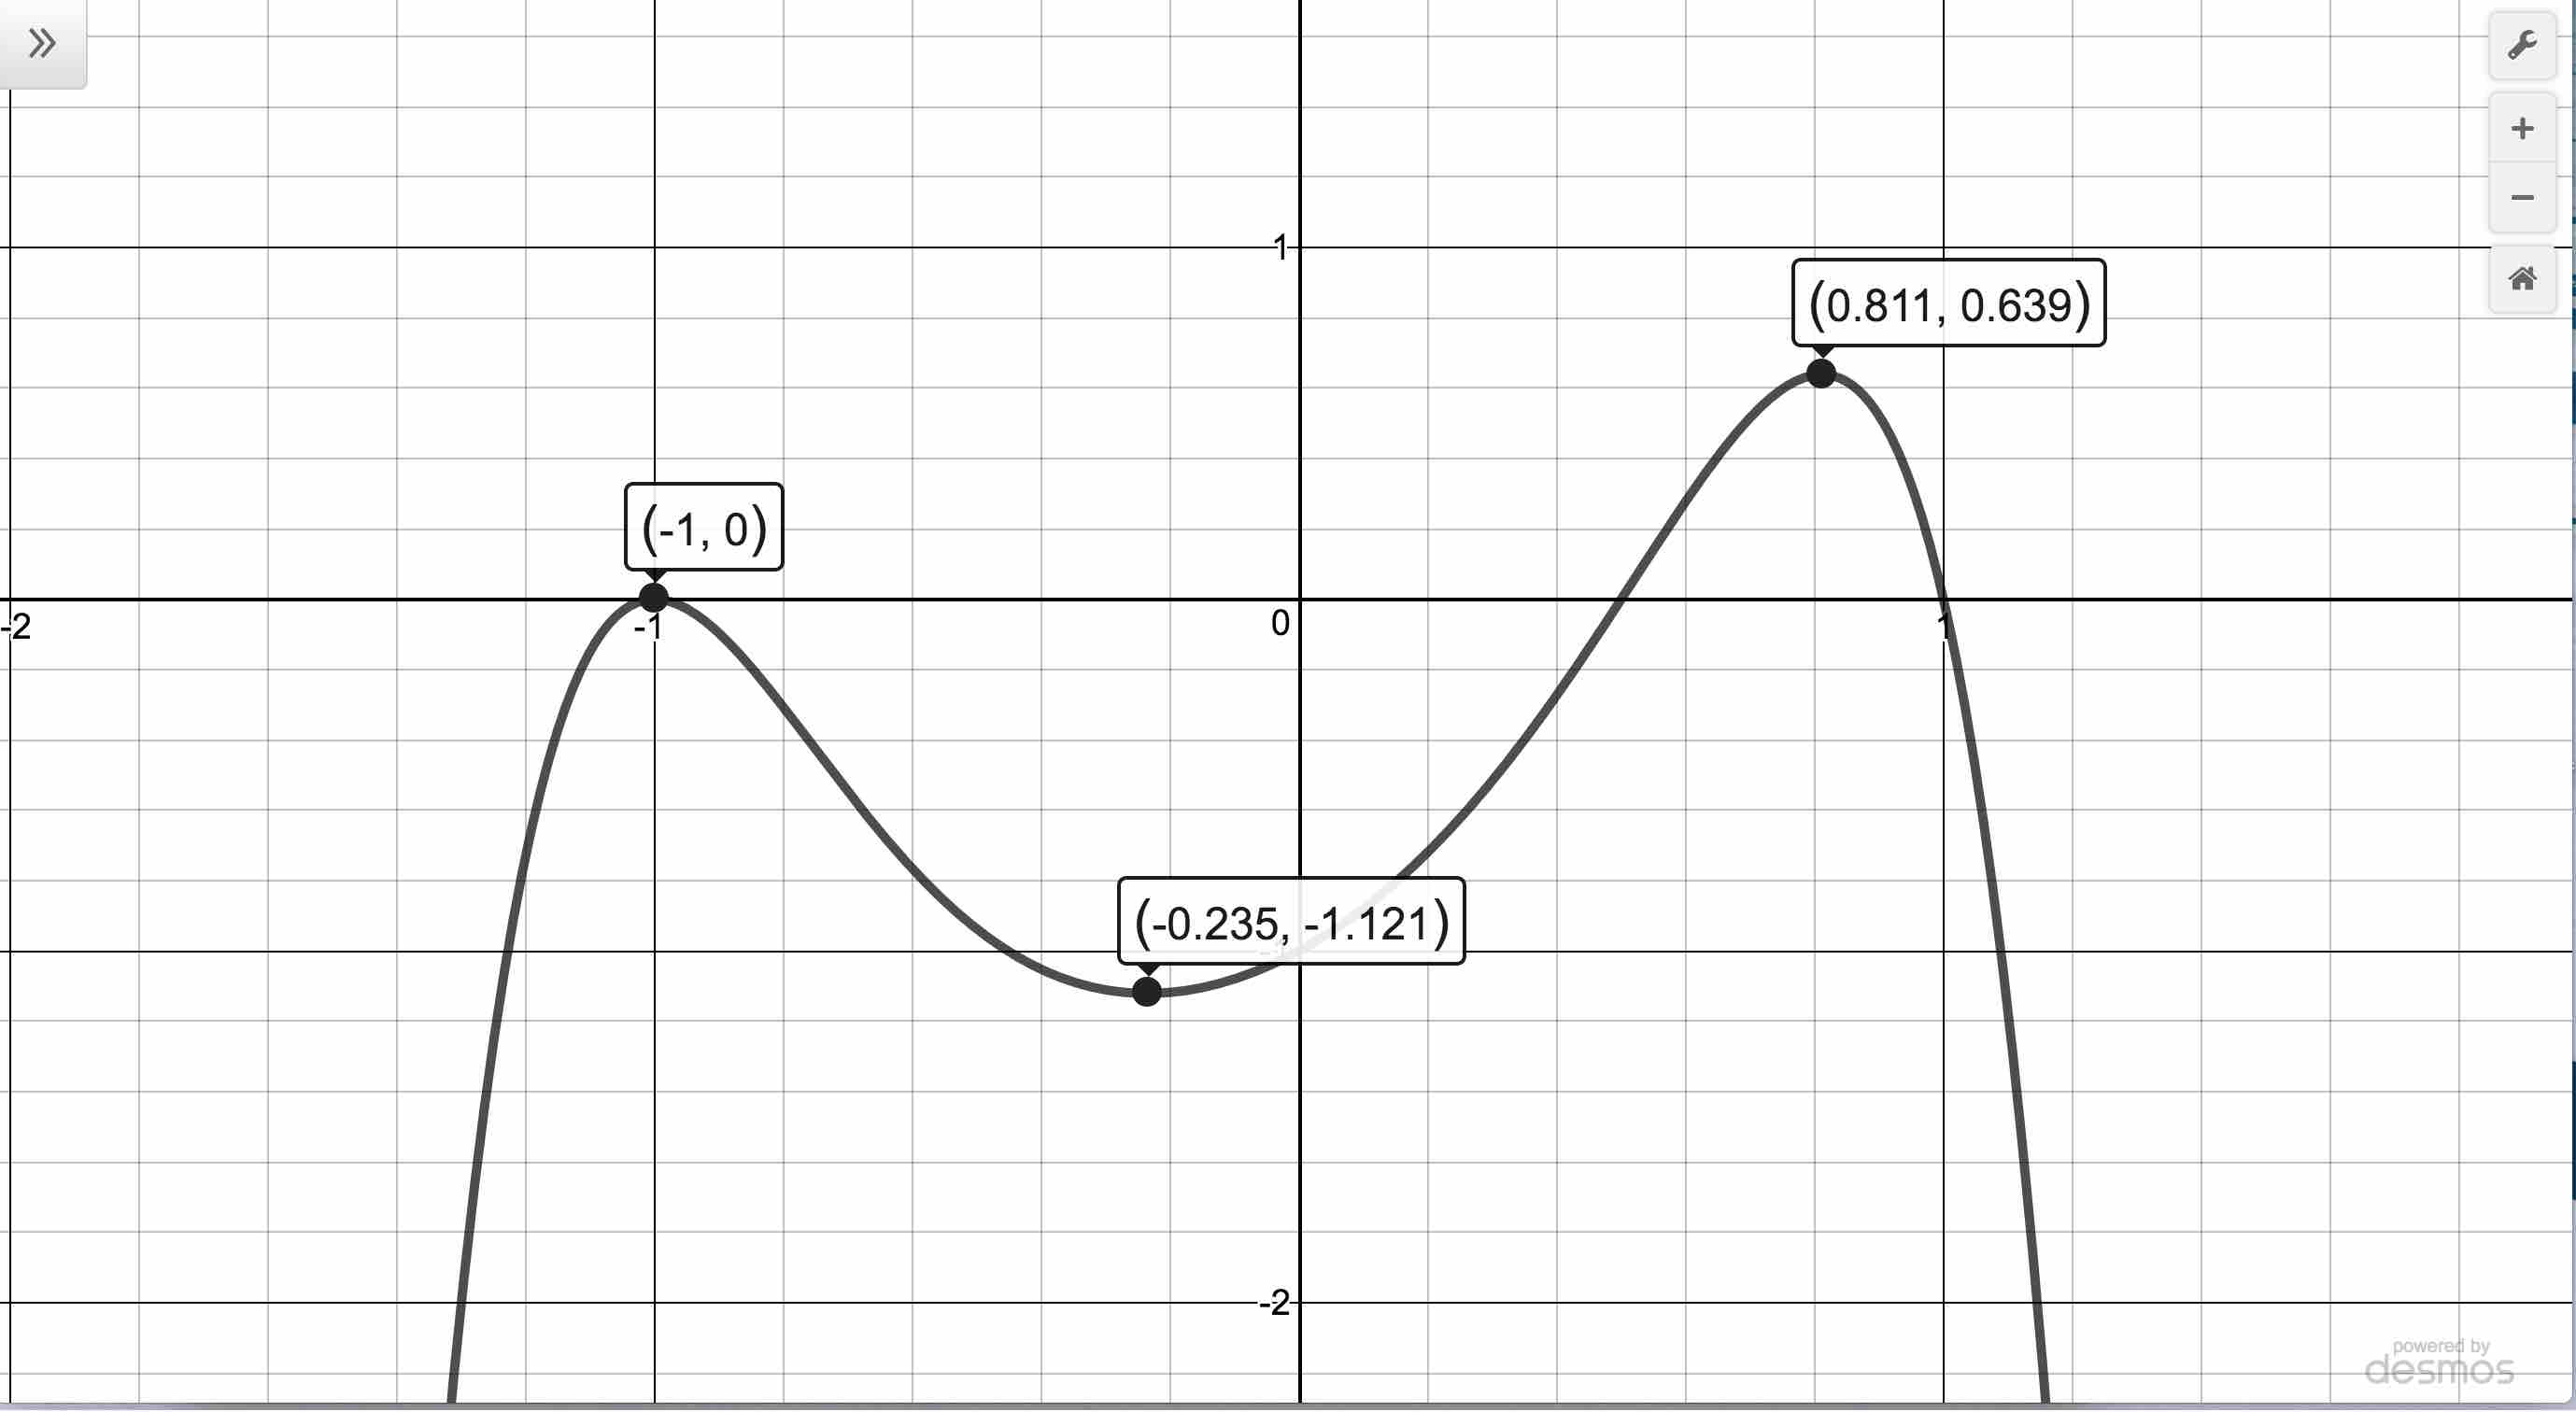
\includegraphics[width=6in]{./GraphsofPolynomialsGraphics/PolyRelativeExtrema.jpg} 

\end{center}



We close this section with a classic application of a third degree polynomial function.

\begin{ex}  \label{boxnotopex} A box with no top is to be fashioned from a $10$ inch $\times$ $12$ inch piece of cardboard by cutting out congruent squares from each corner of the cardboard and then folding the resulting tabs.  Let $x$ denote the length of the side of the square which is removed from each corner.

\bigskip

\begin{tabular}{m{1in}m{2.5in}m{2.5in}} 

&

\begin{mfpic}[15]{-2}{6}{-2}{7}
\hatchcolor[gray]{.7}
\lhatch \rect{(0,0),(1,1)}
\lhatch \rect{(0,5),(1,6)}
\lhatch \rect{(4,5),(5,6)}
\lhatch \rect{(4,0),(5,1)}
\polyline{(0,0),(5,0),(5,6),(0,6),(0,0)}
\dashed \polyline{(1,0),(1,1),(0,1)}
\dashed \polyline{(4,0),(4,1),(5,1)}
\dashed \polyline{(5,5),(4,5),(4,6)}
\dashed \polyline{(0,5),(1,5),(1,6)}
\dotted \polyline{(1,1),(4,1),(4,5),(1,5),(1,1)}
\tlabel[cc](0.5,1.25){\tiny $x$}
\tlabel[cc](1.25,0.5){\tiny $x$}
\tlabel[cc](4.5,1.25){\tiny $x$}
\tlabel[cc](3.75,0.5){\tiny $x$}
\tlabel[cc](4.5,4.75){\tiny $x$}
\tlabel[cc](3.75,5.5){\tiny $x$}
\tlabel[cc](0.5,4.75){\tiny $x$}
\tlabel[cc](1.25,5.5){\tiny $x$}
\arrow \reverse \arrow \polyline{(0,-0.5),(5,-0.5)}
\tlabel[cc](2.5,-1){\tiny $10$ in}
\arrow \reverse \arrow \polyline{(-0.5,0),(-0.5,6)}
\tlabel[cc](-1.5,3){\tiny $12$ in}
\end{mfpic}  & 

\begin{mfpic}[15]{-2}{8}{-2}{4}
\dashed \polyline{(0,1),(0,0)}
\dashed \polyline{(4,0), (4,1)}
\polyline{(0,1),(2,3)}
\polyline{(4,1),(6,3)}
\dotted \polyline{(0,0),(4,0)}
\polyline{(0,1),(4,1)}
\polyline{(2,3),(6,3)}
\dotted \polyline{(4,0),(6,2)}
\dashed \polyline{(6,3),(6,2)}
\dashed \polyline{(2,3),(2,2)}
\dotted \polyline{(2,2),(6,2)}
\dotted \polyline{(2,2),(0,0)}
\arrow \reverse \arrow \polyline{(0,-0.5),(4,-0.5)}
\tlabel[cc](2,-1){\tiny width}
\arrow \reverse \arrow \polyline{(-0.5,0), (-0.5,1)}
\tlabel[cc](-1.5,0.5){\tiny height}
\arrow \reverse \arrow \polyline{(4.5, -0.25), (6.5,1.75)}
\tlabel[cc](6,0.25){\tiny depth}
\end{mfpic}

\end{tabular}

\begin{enumerate}

\item  Find an expression for $V(x)$, the volume of the box produced by removing squares of edge length $x$. Include an appropriate domain.

\item  Use a graphing utility to help you determine the value of $x$ which produces the box with the largest volume.  What is the largest volume?  Round your answers to two decimal places.

\end{enumerate}

{\bf Solution.} 

\begin{enumerate}

\item  From Geometry, we know that $\text{Volume} = \text{width} \times \text{height} \times \text{depth}$.  The key is to find each of these quantities in terms of $x$.  From the figure, we see that the height of the box is $x$ itself.  The cardboard piece is initially $10$ inches wide.  Removing squares with a side length of $x$ inches from each corner leaves $10-2x$ inches for the width.\footnote{There's no harm in taking an extra step here and making sure this makes sense.  If we chopped out a $1$ inch square from each side, then the width would be $8$ inches, so chopping out $x$ inches would leave $10-2x$ inches.}  As for the depth, the cardboard is initially $12$ inches long, so after cutting out $x$ inches from each side, we would have $12-2x$ inches remaining. Hence, we get $V(x) = x(10-2x)(12-2x)$.  To find a suitable applied domain, we note that to make a box at all we need $x > 0$.  Also the shorter of the two dimensions of the cardboard is $10$ inches, and since we are removing $2x$ inches from this dimension, we also require $10 - 2x > 0$ or $x < 5$.  Hence, our applied domain is $0 < x < 5$.

\item  Using a graphing utility, we find a local maximum at approximately $(1.811, 96.771)$.  Because the domain of $V$ is restricted to the interval $(0,5)$,  the maximum of $V$ is here as well.

\begin{center}

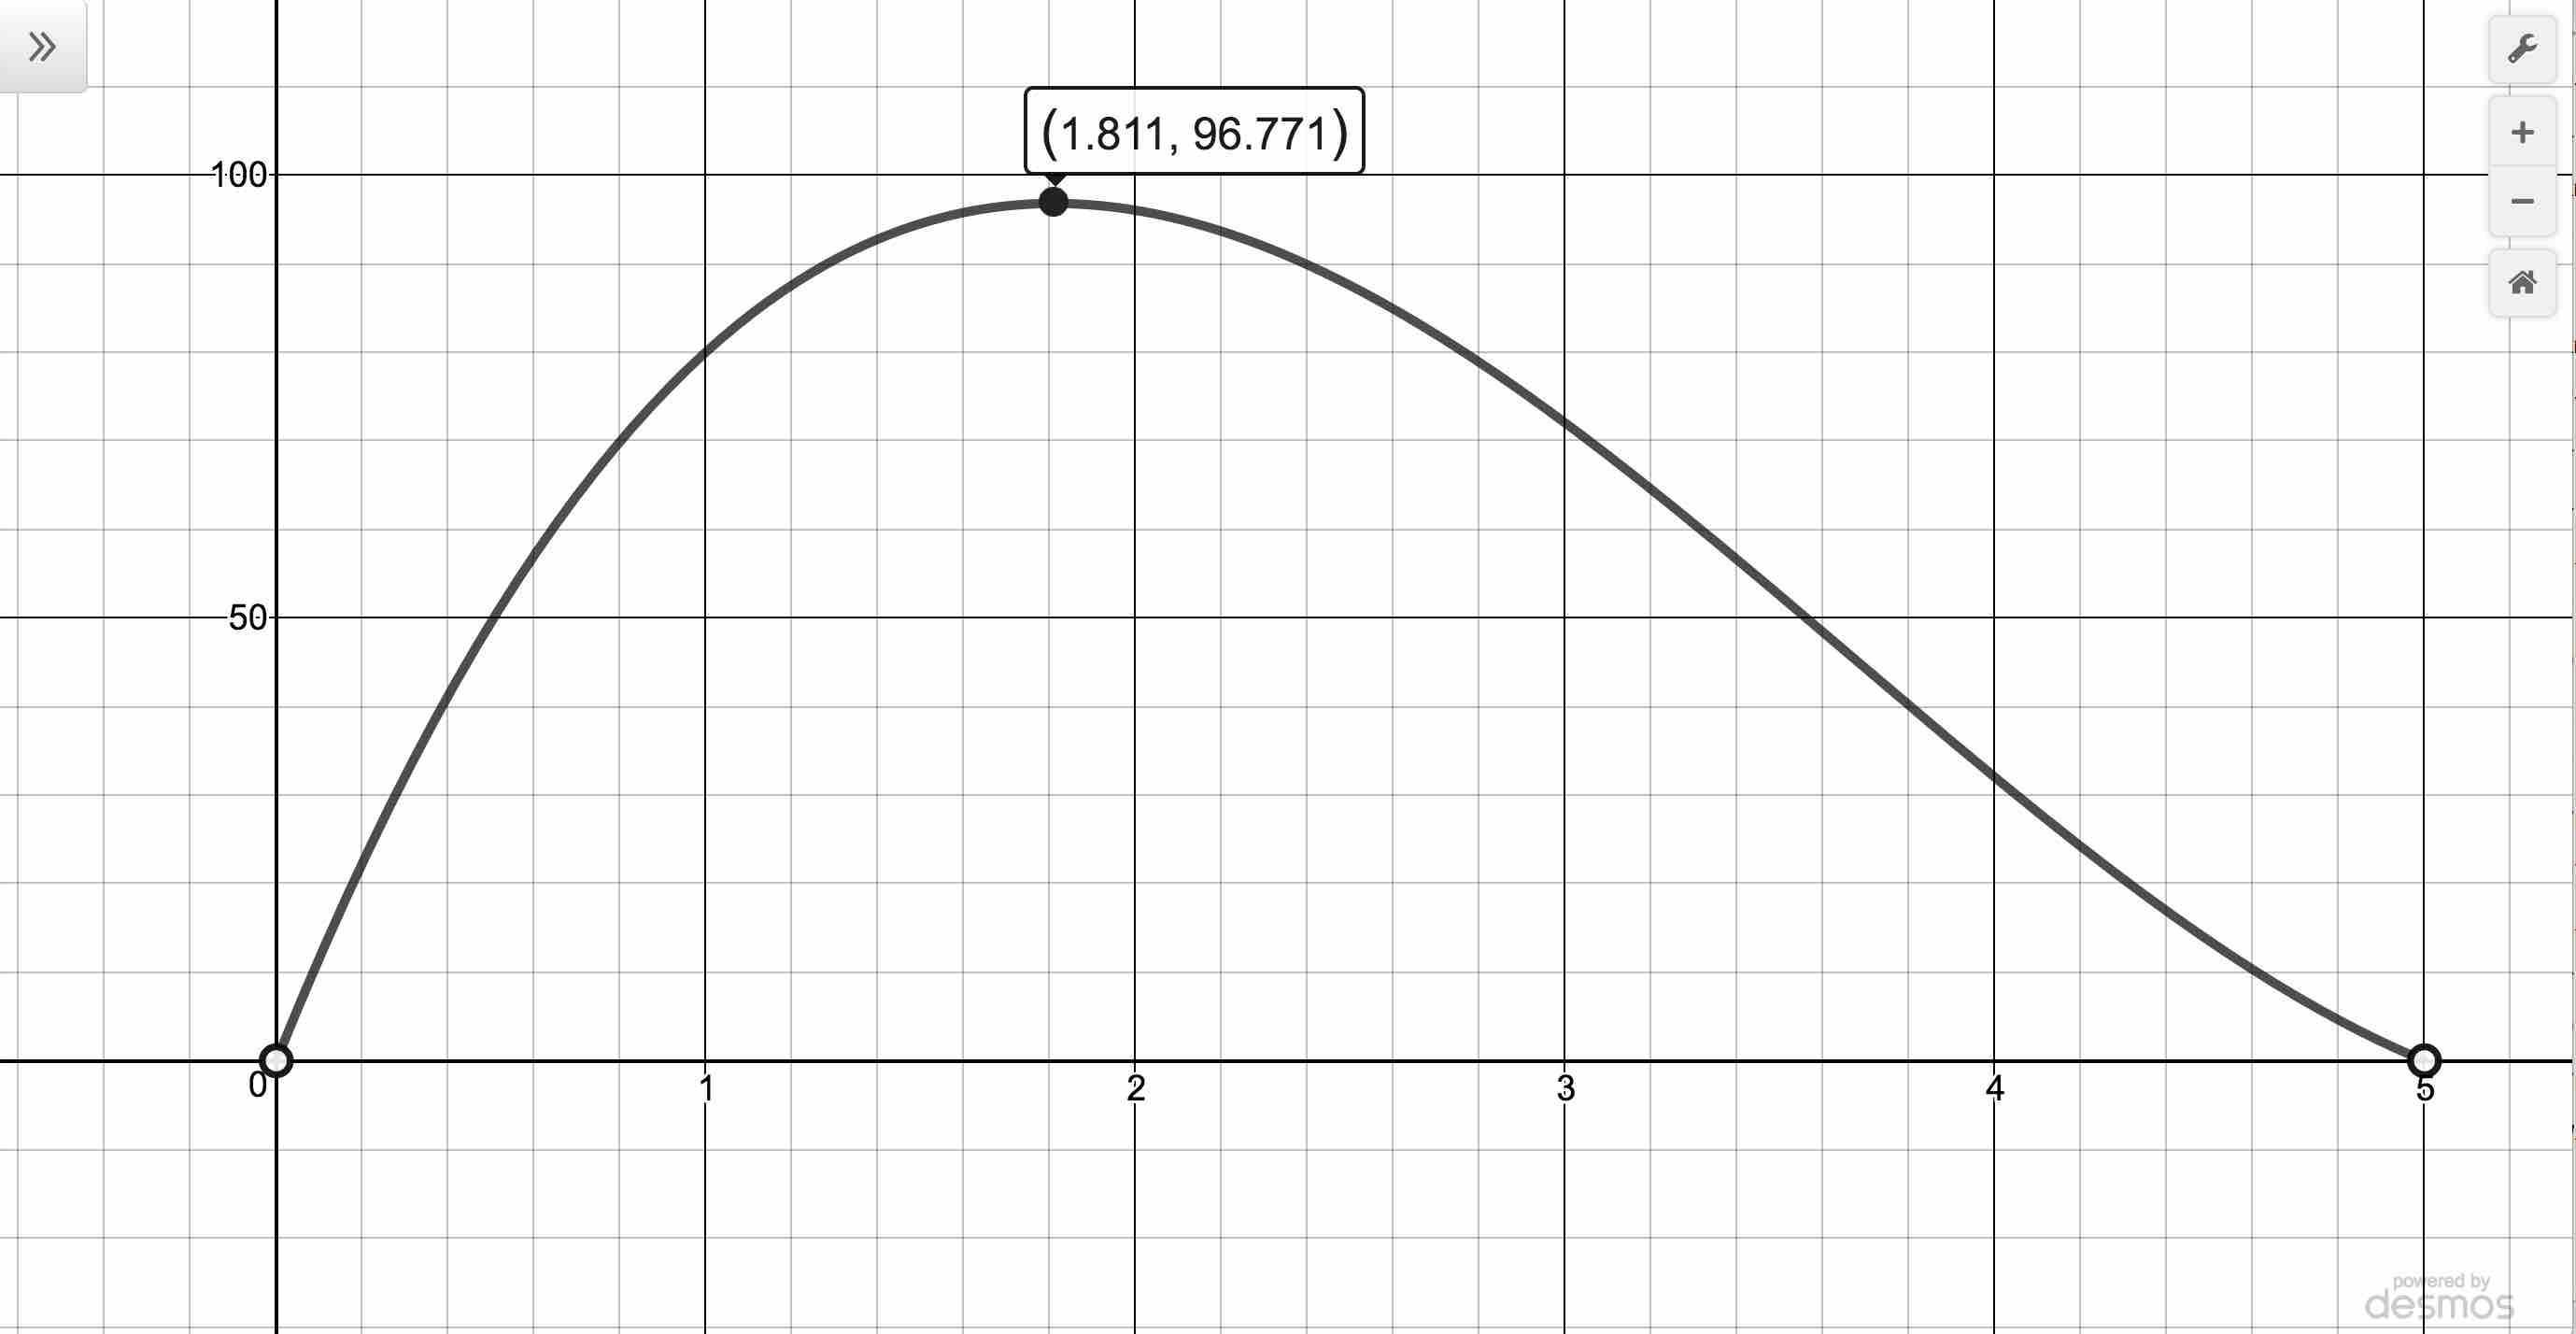
\includegraphics[width=6in]{./GraphsofPolynomialsGraphics/PolyBoxExample.jpg} 

\end{center}

This means the maximum volume attainable is approximately $96.77$ cubic inches when we remove squares approximately $1.81$ inches per side.\qed
 
\end{enumerate}
\label{openbox}
\end{ex}

Notice that there is a very slight, but important, difference between the function $V(x) = x(10-2x)(12-2x)$, $0 < x < 5$ from Example  \ref{boxnotopex} and the function $p(x) = x(10-2x)(12-2x)$: their domains.  The domain of $V$ is restricted to the interval $(0,5)$ while the domain of $p$ is $(-\infty, \infty)$.  Indeed, the function $V$ has a maximum of (approximately) $96.771$ at (approximately) $x = 1.811$ whereas for the function $p$, $96.771$ is a local maximum value only.  We leave it to the reader to verify that $V$ has neither a minimum nor a local minimum.

\newpage

\subsection{Exercises}

In Exercises \ref{polytransfirst} - \ref{polytranslast}, given the pair of functions $f$ and $F$, sketch the graph of $y=F(x)$ by starting with the graph of $y = f(x)$ and using Theorem \ref{linearmononialgraphs}.  Track at least three points of your choice through the transformations. State the domain and range of $g$.

\begin{multicols}{2}
\begin{enumerate}


\item $f(x) = x^3$,  $F(x) = (x + 2)^{3} + 1$ \label{polytransfirst}
\item $f(x) = x^4$, $F(x) = (x + 2)^{4} + 1$

\setcounter{HW}{\value{enumi}}
\end{enumerate}
\end{multicols}

\begin{multicols}{2}
\begin{enumerate}
\setcounter{enumi}{\value{HW}}

\item $f(x) = x^4$, $F(x) = 2 - 3(x - 1)^{4}$
\item $f(x) = x^5$, $F(x) = -x^{5} - 3$

\setcounter{HW}{\value{enumi}}
\end{enumerate}
\end{multicols}

\begin{multicols}{2}
\begin{enumerate}
\setcounter{enumi}{\value{HW}}

\item $f(x) = x^5$, $F(x) = (x+1)^5+10$
\item $f(x) = x^6$, $F(x) = 8-x^6$ \label{polytranslast}

\setcounter{HW}{\value{enumi}}
\end{enumerate}
\end{multicols}


In Exercises \ref{findformulaforcubicgraphfirst} - \ref{findformulacubicgraphlast}, find a formula for each function below in the form $F(x) = a(x-h)^3+k$.

\begin{multicols}{2}

\begin{enumerate}
\setcounter{enumi}{\value{HW}}

\item $~$ \label{findformulaforcubicgraphfirst}

\begin{mfpic}[15]{-5}{5}{-5}{5}
\axes
\tlabel[cc](5,-0.5){\scriptsize $x$}
\tlabel[cc](0.5,5){\scriptsize $y$}
\tlabel[cc](-1.25, -3){\scriptsize $(0,-3)$}
\tlabel[cc](1.25,-2.75){\scriptsize $(1,-2)$}
\xmarks{-4,-3,-2,-1,1,2,3,4}
\ymarks{-4,-3,-2, -1, 1,2,3,4}
\tlpointsep{4pt}
\scriptsize
\axislabels {x}{ {$-4 \hspace{7pt}$} -4, {$-3 \hspace{7pt}$} -3, {$-2 \hspace{7pt}$} -2, {$-1 \hspace{7pt}$} -1, {$1$} 1, {$2$} 2, {$3$} 3, {$4$} 4}
\axislabels {y}{{$-1$} -1,{$1$} 1, {$2$} 2, {$3$} 3, {$4$} 4, {$-2$} -2}
\penwd{1.25pt}
\arrow \reverse \arrow \function{-0.4,2.9,0.1}{(x-1)**3-2}
\point[4pt]{(1,-2), (0,-3)}
\tcaption{ \scriptsize$y = F(x)$}
\normalsize
\end{mfpic} 



\item $~$ \label{findformulacubicgraphlast}

\begin{mfpic}[15]{-5}{5}{-5}{5}
\axes
\tlabel[cc](5,-0.5){\scriptsize $x$}
\tlabel[cc](0.5,5){\scriptsize $y$}
\tlabel[cc](1,-1){\scriptsize $(0,-1)$}
\tlabel[cc](-2.25,2.25){\scriptsize $(-2,3)$}
\xmarks{-4,-3,-2,-1,1,2,3,4}
\ymarks{-4,-3,-2, -1, 1,2,3,4}
\tlpointsep{4pt}
\scriptsize
\axislabels {x}{ {$-4 \hspace{7pt}$} -4, {$-3 \hspace{7pt}$} -3, {$-2 \hspace{7pt}$} -2, {$-1 \hspace{7pt}$} -1, {$1$} 1, {$2$} 2, {$3$} 3, {$4$} 4}
\axislabels {y}{{$-1$} -1, {$2$} 2, {$3$} 3, {$4$} 4, {$-2$} -2, {$-3$} -3, {$-4$} -4}
\penwd{1.25pt}
\arrow \reverse \arrow \function{-3.5,0.5,0.1}{3-(0.5*((x+2)**3))}
\point[4pt]{(-2,3), (0,-1)}
\tcaption{ \scriptsize$y = F(x)$}
\normalsize
\end{mfpic} 

\setcounter{HW}{\value{enumi}}

\end{enumerate}

\end{multicols}

In Exercises \ref{findformulaforquartgraphfirst} - \ref{findformulaquartgraphlast}, find a formula for each function below in the form $F(x) = a(x-h)^4+k$.


\begin{multicols}{2}

\begin{enumerate}

\setcounter{enumi}{\value{HW}}

\item $~$ \label{findformulaforquartgraphfirst}

\begin{mfpic}[15]{-5}{5}{-5}{5}
\axes
\tlabel[cc](5,-0.5){\scriptsize $x$}
\tlabel[cc](0.5,5){\scriptsize $y$}
\tlabel[cc](-1.25,-4.5){\scriptsize $(-1,-4)$}
\tlabel[cc](1,-2){\scriptsize $(0,-2)$}
\xmarks{-4,-3,-2,-1,1,2,3,4}
\ymarks{-4,-3,-2, -1, 1,2,3,4}
\tlpointsep{4pt}
\scriptsize
\axislabels {x}{ {$-4 \hspace{7pt}$} -4, {$-3 \hspace{7pt}$} -3, {$-1 \hspace{7pt}$} -1, {$1$} 1, {$2$} 2,{$3$} 3, {$4$} 4}
\axislabels {y}{{$-1$} -1,{$1$} 1, {$2$} 2, {$3$} 3,  {$-2$} -2, {$-3$} -3, {$4$} 4}
\penwd{1.25pt}
\arrow \reverse \arrow \function{-2.41,0.41,0.1}{2*((x+1)**4)-4}
\point[4pt]{(-1,-4), (0,-2)}
\tcaption{ \scriptsize$y = F(x)$}
\normalsize
\end{mfpic} 



\item $~$  \label{findformulaquartgraphlast}

\begin{mfpic}[15]{-5}{5}{-5}{5}
\axes
\tlabel[cc](5,-0.5){\scriptsize $x$}
\tlabel[cc](0.5,5){\scriptsize $y$}
\tlabel[cc](-3,0.5){\scriptsize $(-2,0)$}
\tlabel[cc](2.5,0.5){\scriptsize $(2,0)$}
\tlabel[cc](-2,2.5){\scriptsize $(0,2.5)$}
\xmarks{-4,-3,-2,-1,1,2,3,4}
\ymarks{-4,-3,-2, -1, 1,2,3,4}
\tlpointsep{4pt}
\scriptsize
\axislabels {x}{ {$-4 \hspace{7pt}$} -4, {$-3 \hspace{7pt}$} -3, {$-1 \hspace{7pt}$} -1,  {$1$} 1, {$3$} 3, {$4$} 4}
\axislabels {y}{{$-1$} -1,{$-2$} -2,{$-3$} -3,{$-4$} -4,{$1$} 1, {$2$} 2, {$3$} 3,  {$4$} 4}
\penwd{1.25pt}
\arrow \reverse \arrow \function{-2.5,2.5,0.1}{2.5-(0.1565*(x**4))}
\point[4pt]{(-2,0), (2,0), (0, 2.5)}
\tcaption{ \scriptsize$y = F(x)$}
\normalsize
\end{mfpic} 


\setcounter{HW}{\value{enumi}}

\end{enumerate}

\end{multicols}


In Exercises \ref{polyfactsfirst} - \ref{polyfactslast}, find the degree, the leading term, the leading coefficient, the constant term and the end behavior of the given polynomial function.

\begin{multicols}{2}
\begin{enumerate}
\setcounter{enumi}{\value{HW}}
\item  $f(x) = 4-x-3x^2$ \label{polyfactsfirst}
\item  $g(x) = 3x^5 - 2x^2 + x + 1$

\setcounter{HW}{\value{enumi}}
\end{enumerate}
\end{multicols}

\begin{multicols}{2}
\begin{enumerate}
\setcounter{enumi}{\value{HW}}

\item $q(r) = 1 - 16r^{4}$
\item $Z(b) = 42b - b^{3}$

\setcounter{HW}{\value{enumi}}
\end{enumerate}
\end{multicols}

\begin{multicols}{2}
\begin{enumerate}
\setcounter{enumi}{\value{HW}}

\item $f(x) = \sqrt{3}x^{17} + 22.5x^{10} - \pi x^{7} + \frac{1}{3}$
\item $s(t) = -4.9t^{2} + v_{\mbox{\tiny $0$}}t + s_{\mbox{\tiny $0$}}$

\setcounter{HW}{\value{enumi}}
\end{enumerate}
\end{multicols}

\begin{multicols}{2}
\begin{enumerate}
\setcounter{enumi}{\value{HW}}

\item $P(x) = (x - 1)(x - 2)(x - 3)(x - 4)$
\item $p(t) = -t^2(3 - 5t)(t^{2} + t + 4)$

\setcounter{HW}{\value{enumi}}
\end{enumerate}
\end{multicols}

\begin{multicols}{2}
\begin{enumerate}
\setcounter{enumi}{\value{HW}}

\item $f(x) = -2x^3(x+1)(x+2)^2$
\item $G(t) = 4(t-2)^2\left(t+\frac{1}{2}\right)$ \label{polyfactslast}

\setcounter{HW}{\value{enumi}}
\end{enumerate}
\end{multicols}

\phantomsection
\label{polygraphexercise}

In Exercises \ref{zeromultgraphfirst} - \ref{zeromultgraphlast}, find the real zeros of the given polynomial and their corresponding multiplicities.  Use this information along with end behavior to provide a rough sketch of the graph of the polynomial function.  Compare your answer with the result from a graphing utility.

\begin{multicols}{2}
\begin{enumerate}
\setcounter{enumi}{\value{HW}}

\item $a(x) = x(x + 2)^{2}$ \label{zeromultgraphfirst}
\item $g(t) = t(t + 2)^{3}$

\setcounter{HW}{\value{enumi}}
\end{enumerate}
\end{multicols}


\begin{multicols}{2}
\begin{enumerate}
\setcounter{enumi}{\value{HW}}

\item $f(z) = -2(z-2)^2(z+1)$
\item $g(x) = (2x+1)^2(x-3)$

\setcounter{HW}{\value{enumi}}
\end{enumerate}
\end{multicols}


\begin{multicols}{2}
\begin{enumerate}
\setcounter{enumi}{\value{HW}}

\item $F(t) = t^{3}(t+ 2)^{2}$
\item $P(z) = (z- 1)(z - 2)(z - 3)(z - 4)$

\setcounter{HW}{\value{enumi}}
\end{enumerate}
\end{multicols}


\begin{multicols}{2}
\begin{enumerate}
\setcounter{enumi}{\value{HW}}

\item $Q(x) = (x + 5)^{2}(x - 3)^{4}$
\item $h(t) = t^2(t-2)^2(t+2)^2$

\setcounter{HW}{\value{enumi}}
\end{enumerate}
\end{multicols}


\begin{multicols}{2}
\begin{enumerate}
\setcounter{enumi}{\value{HW}}

\item $H(z) = (3-z)(z^2+1)$
\item $Z(x) = x(42 - x^{2})$ \label{zeromultgraphlast}

\setcounter{HW}{\value{enumi}}
\end{enumerate}
\end{multicols}

In Exercises \ref{evenoddornotpolyfirst} - \ref{evenoddornotpolylast}, determine analytically if the following functions are even, odd or neither.  Confirm your answer using a graphing utility.


\begin{multicols}{3}
\begin{enumerate}
\setcounter{enumi}{\value{HW}}

\item $f(x) = 7x$ \label{evenoddornotpolyfirst}
\item $g(t) = 7t + 2$
\item $p(z) = 7$

\setcounter{HW}{\value{enumi}}
\end{enumerate}
\end{multicols}

\begin{multicols}{3}
\begin{enumerate}
\setcounter{enumi}{\value{HW}}

\item $F(s) = 3s^2 - 4$
\item $h(t) = 4-t^2$
\item $g(x) = x^2-x-6$

\setcounter{HW}{\value{enumi}}
\end{enumerate}
\end{multicols}


\begin{multicols}{3}
\begin{enumerate}
\setcounter{enumi}{\value{HW}}

\item $f(x) = 2x^3 - x$
\item $p(z) = -z^5 + 2z^3 - z$
\item $G(t) = t^{6} - t^{4} + t^{2} + 9$

\setcounter{HW}{\value{enumi}}
\end{enumerate}
\end{multicols}

\begin{multicols}{3}
\begin{enumerate}
\setcounter{enumi}{\value{HW}}

\item $G(s) = s(s^2 - 1)$
\item $f(x) = (x^2+1)(x-1)$
\item $H(t) = (t^2-1)(t^4+t^2+3)$

\setcounter{HW}{\value{enumi}}
\end{enumerate}
\end{multicols}

\begin{multicols}{3}
\begin{enumerate}
\setcounter{enumi}{\value{HW}}

\item $g(t) = t(t-2)(t+2)$
\item $P(z) = (2z^{5} - 3z)(5z^3+z)$ 
\item $f(x) =0$  \label{evenoddornotpolylast}

\setcounter{HW}{\value{enumi}}
\end{enumerate}
\end{multicols}


\begin{enumerate}
\setcounter{enumi}{\value{HW}}

\item  \label{evenoddpolynomialexercise} Suppose $p(x)$ is a polynomial function written in the form of  Definition \ref{polynomialfunction}.  

\begin{enumerate}

\item  If the nonzero terms of $p(x)$ consist of even powers of $x$ (or a constant), explain why $p$ is even.

\item   If the nonzero terms of $p(x)$ consist of odd powers of $x$, explain why $p$ is odd.

\item  If $p(x)$ the nonzero terms of $p(x)$  contain at least one odd power of $x$ and one even power of $x$ (or a constant term), then $p$ is neither even nor odd.

\end{enumerate}

\newpage

\item  Use the results of Exercise \ref{evenoddpolynomialexercise} to determine whether the following functions are even, odd, or neither.

\begin{multicols}{4}
\begin{enumerate}

\item  $p(x) = 3x^4 + x^2 - 1$

\item  $F(s) = s^3 - 14s$

\item  $f(t) = 2t^5 - t^2 + 1$

\item  $g(x) =x^3(x^2+1)$

\end{enumerate}

\end{multicols}

\item  Show  $f(x) = |x|$ is an even function.


\item  Rework Example \ref{boxnotopex} assuming the box is to be made from an 8.5 inch by 11 inch sheet of paper. Using scissors and tape, construct the box.  Are you surprised?\footnote{Consider decorating the box and presenting it to your instructor. If done well enough, maybe your instructor will issue you some bonus points.  Or maybe not.}

\item For each function $f(x)$ listed below, compute the average rate of change over the indicated interval.\footnote{See Definition \ref{arc} in Section \ref{AverageRateofChange} for a review of this concept, as needed.}  What trends do you observe?  How do your answers manifest themselves graphically?

\[ \begin{array}{|r||c|c|c|c|c|c|}  \hline

 f(x) &  [-0.1, 0] & [0, 0.1] &[0.9, 1] & [1, 1.1] & [1.9, 2] & [2, 2.1]  \\ \hline
 1 &&&&&& \\  \hline
 x  &&&&&& \\  \hline
 x^2 &&&&&&  \\  \hline
 x^3 &&&&&& \\  \hline
 x^4 &&&&&& \\ \hline
 x^5 &&&&&& \\ \hline

\end{array} \]


\item \label{monomialarcexercise}For each function $f(x)$ listed below, compute the average rate of change over the indicated interval.\footnote{See Definition \ref{arc} in Section \ref{AverageRateofChange} for a review of this concept, as needed.}  What trends do you observe?  How do your answers manifest themselves graphically?

\[ \begin{array}{|r||c|c|c|c|}  \hline

 f(x) &  [0.9, 1.1] & [0.99, 1.01] &[0.999, 1.001] & [0.9999, 1.0001]  \\ \hline
 1 &&&&   \\  \hline
 x &&&&    \\  \hline
 x^2 &&&&   \\  \hline
 x^3 &&&&   \\  \hline
 x^4 &&&&  \\ \hline
 x^5 &&&&  \\ \hline

\end{array} \]




\setcounter{HW}{\value{enumi}}
\end{enumerate}

\phantomsection
\label{LCDmaxprofit} 

In Exercises \ref{lcdmaxprofitexerfirst} - \ref{lcdmaxprofitexerlast}, suppose the revenue $R$, in \textit{thousands} of dollars, from producing and selling $x$ \textit{hundred} LCD TVs is given by $R(x) = -5x^3+35x^2+155x$ for $0 \leq x \leq 10.07$.

\begin{enumerate}
\setcounter{enumi}{\value{HW}}

\item  Use a graphing utility to graph $y = R(x)$ and determine the number of TVs which should be sold to maximize revenue.  What is the maximum revenue? \label{lcdmaxprofitexerfirst}

\item Assume the cost, in \textit{thousands} of dollars, to produce $x$ \textit{hundred} LCD TVs is given by the function $C(x) = 200x + 25$ for $x \geq 0$. Find and simplify an expression for the profit function $P(x)$.  

(Remember: Profit = Revenue - Cost.)

\item  Use a graphing utility to graph $y = P(x)$ and determine the number of TVs which should be sold to maximize profit.  What is the maximum  profit? \label{lcdmaxprofitexerlast}

\item \label{newportaboycost} While developing their newest game, Sasquatch Attack!, the makers of the PortaBoy (from Example \ref{PortaBoyCost}) revised their cost function and now use $C(x) = .03x^{3} - 4.5x^{2} + 225x + 250$, for $x \geq 0$. As before, $C(x)$ is the cost to make $x$ PortaBoy Game Systems.  Market research indicates that the demand function $p(x) = -1.5x + 250$ remains unchanged.  Use a graphing utility to find the production level $x$ that maximizes the \textit{profit} made by producing and selling $x$ PortaBoy game systems.

\setcounter{HW}{\value{enumi}}
\end{enumerate}

\begin{enumerate}
\setcounter{enumi}{\value{HW}}

\item According to US Postal regulations, a rectangular shipping box must satisfy the following inequality: ``Length + Girth $\leq$ 130 inches'' for Parcel Post and ``Length + Girth $\leq$ 108 inches'' for other services. 

\smallskip

Let's assume we have a closed rectangular box with a square face of side length $x$ as drawn below.  The length is the longest side and is clearly labeled.  The girth is the distance around the box in the other two dimensions so in our case it is the sum of the four sides of the square, $4x$.  

\begin{enumerate}

\item \label{girthbox1} Assuming that we'll be mailing a box via Parcel Post where Length + Girth $=$ 130 inches, express the length of the box in terms of $x$ and then express the volume $V$ of the box in terms of $x$.

\item \label{girthbox2} Find the dimensions of the box of maximum volume that can be shipped via Parcel Post.

\item Repeat parts \ref{girthbox1} and \ref{girthbox2} if the box is shipped using ``other services''.

\end{enumerate}

\begin{center}

\begin{mfpic}[8]{-6}{12}{-1}{17}
\polyline{(0,0),(-4,3)}
\polyline{(-4,3), (-4,8)}
\polyline{(-4,8),(0,5)}
\polyline{(0,5),(0,0)}
\polyline{(0,0),(12,9)}
\polyline{(0,5),(12,14)}
\polyline{(-4,8),(8,17)}
\polyline{(8,17),(12,14)}
\polyline{(12,14),(12,9)}
\arrow \reverse \arrow \polyline{(0,-0.5),(12,8.5)}
\tlabel[cc](8,4){\tiny length}
\arrow \reverse \arrow \polyline{(-4, 2.5), (-0.5,-0.125)}
\tlabel[cc](-3,0.5){\tiny $x$}
\arrow \reverse \arrow \polyline{(-4.5, 3), (-4.5,8)}
\tlabel[cc](-5,5){\tiny $x$}
\end{mfpic}

\end{center}

\setcounter{HW}{\value{enumi}}
\end{enumerate}

\newpage

\begin{enumerate}
\setcounter{enumi}{\value{HW}}


\item \label{sunlighthigherorder} This exercise revisits the data set from Exercise \ref{regsunlight} in Section \ref{QuadraticFunctions}.  In that exercise, you were given a chart of the number of hours of daylight they get on the $21^{\mbox{st}}$ of each month in Fairbanks, Alaska based on the 2009 sunrise and sunset data found on the  \href{http://aa.usno.navy.mil/data/docs/RS_OneYear.php}{\underline{U.S. Naval Observatory}} website.  Here  $x = 1$ represents January 21, 2009, $x = 2$ represents February 21, 2009, and so on.  
\medskip

\small

\noindent \begin{tabular}{|l|r|r|r|r|r|r|r|r|r|r|r|r|} \hline
Month  & & & & & & & & & & & & \\
Number & 1 & 2 & 3 & 4 & 5 & 6 & 7 & 8 & 9 & 10 & 11 & 12\\ 
\hline 
Hours of  & & & & & & & & & & & & \\
Daylight & 5.8 & 9.3 & 12.4 & 15.9 & 19.4 & 21.8 & 19.4 & 15.6 & 12.4 & 9.1 & 5.6 & 3.3 \\ \hline
\end{tabular}

\normalsize

\medskip

\noindent 

\begin{itemize}

\item Find cubic (third degree) and quartic (fourth degree) polynomials which model this data and comment on the goodness of fit for each.  What can we say about using either model to make predictions about the year 2020?  (Hint: Think about the end behavior of polynomials.)  

\item Use the models to see how many hours of daylight they got on your birthday and then check the website to see how accurate the models are.  

\item Sasquatch are largely nocturnal, so what days of the year according to your models  allow for at least 14 hours of darkness for field research on the elusive creatures? 

\end{itemize}

\item \label{circuitexercisepoly} An electric circuit is built with a variable resistor installed.  For each of the following resistance values (measured in kilo-ohms, $k \Omega$),  the corresponding power to the load (measured in milliwatts, $mW$) is given in the table below. \footnote{The authors wish to thank Don Anthan and Ken White of Lakeland Community College for devising this problem and generating the accompanying data set.}

\noindent \begin{tabular}{|l|r|r|r|r|r|r|} \hline
Resistance: ($k \Omega$) & 1.012 & 2.199 & 3.275 & 4.676 & 6.805 & 9.975 \\ \hline
Power: ($mW$) & 1.063 & 1.496 & 1.610 & 1.613 & 1.505 & 1.314 \\ \hline
\end{tabular}

\begin{enumerate}

\item Make a scatter diagram of the data using the Resistance as the independent variable and Power as the dependent variable.

\item Use your calculator to find quadratic (2nd degree), cubic (3rd degree) and quartic (4th degree) regression models for the data and judge the reasonableness of each.

\item For each of the models found above, find the predicted maximum power that can be delivered to the load.  What is the corresponding resistance value?

\item Discuss with your classmates the limitations of these models - in particular, discuss the end behavior of each.

\end{enumerate}

\newpage

\item Below is a graph of  a polynomial function $y = p(x)$ as generated by a graphing utility.   Answer the following questions about $p$ based on the graph provided.


\centerline{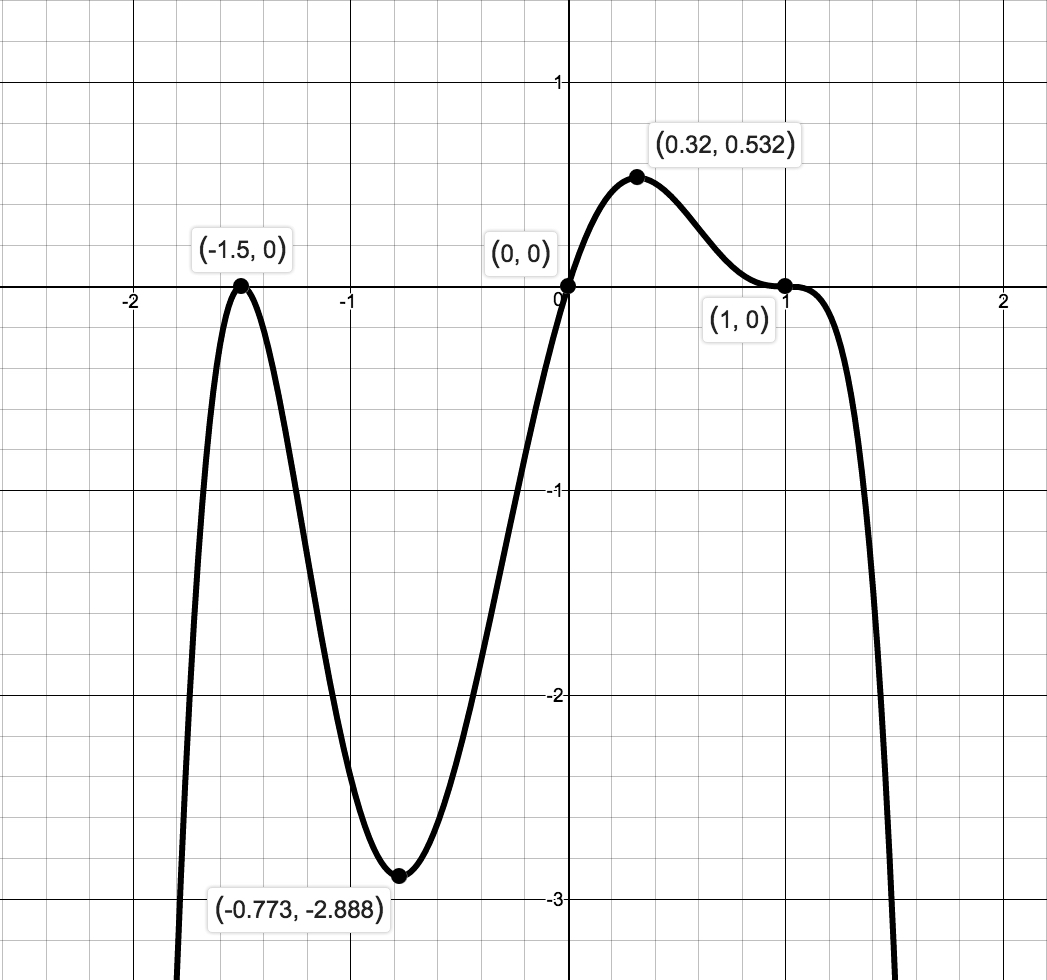
\includegraphics[width=3in]{./GraphsofPolynomialsGraphics/GraphsofPolyExercise.jpg}}

\begin{enumerate}

\item  Describe the end behavior of $y = p(x)$.

\item  List the real zeros of $p$ along with their respective multiplicities.  

\item  List the local minimums and local maximums of the graph of $y = p(x)$.

\item  What can be said about the degree of and leading coefficient $p(x)$?

\item  It turns out that $p(x)$ is a seventh degree polynomial.\footnote{to be exact, $p(x) = -0.1\left(x+1.5\right)^2\left(3x\right)\left(x-1\right)^3\left(x+5\right)$.}  How can this be?

\end{enumerate}

\item  \label{comparegraphfromtheoryexample}  (This Exercise is a follow up to Example \ref{graphfromtheory}.)  Use a graphing utility to  compare and contrast the graphs of $f(x) = (2x-1)(x+1)^2(1-x)(x^2+1)$ and $g(x) = (2x-1)(x+1)^2(1-x)$.

\item Use the graph of $y= p(x) = (2x-1)(x+1)(1-x^4)$ on page \pageref{localmaxminexample} to estimate the largest open interval containing $x = -0.235$ which satisfies the the criteria for `local minimum'  in Definition \ref{localmaxmindefn}.

\item  In light of Definition \ref{localmaxmindefn}, explain why \textit{every} point on the graph of a constant function is both a local maximum and a local minimum.

\item This exercise involves the greatest integer function, $f(x) = \lfloor x \rfloor$,  introduced in Example \ref{greatestintegerdefn}.  Explain why the points $(k,k)$ for integers $k$ are local maximums but not local minimums.

\item  Use Theorems  \ref{EBPolynomials}  and \ref{polynomialbehaviornearzeros} prove Theorem \ref{roleofmultiplicity}.


\newpage

\item Here are a few other questions for you to discuss with your classmates.  

\begin{enumerate}

\item How many and how few  local extrema could a polynomial of degree $n$ have?  
\item Could a polynomial have two local maxima but no local minima?  
\item If a polynomial has two local maxima and two local minima, can it be of odd degree?  Can it be of even degree?
\item Can a polynomial have local extrema without having any real zeros?
\item Why must every polynomial of odd degree have at least one real zero?
\item Can a polynomial have two distinct real zeros and no local extrema?
\item Can an $x$-intercept yield a local extrema?  Can it yield an absolute extrema?
\item If the $y$-intercept yields an absolute minimum, what can we say about the degree of the polynomial and the sign of the leading coefficient?   

\end{enumerate}

\item \label{LagrangePolyExercise} (This is a follow-up to Exercises \ref{LagrangeLinearExercise} in Section \ref{ConstantandLinearFunctions} and \ref{LagrangeQuadExercise} in Section \ref{QuadraticFunctions}.) The  \href{https://en.wikipedia.org/wiki/Lagrange_polynomial}{\underline{Lagrange Interpolate}} function $L$  for four  points:  $(x_{0}, y_{0})$, $(x_{1}, y_{1})$,  $(x_{2}, y_{2})$,   $(x_{3}, y_{3})$ where $x_{0}$,  $x_{1}$, $x_{2}$, and $x_{3}$ are four distinct real numbers is given by the formula: 

 \[ \begin{array}{rcl}
 
 L(x) & = &  y_{0}  \dfrac{(x - x_{1}) (x - x_{2}) (x-x_{3})}{(x_{0} - x_{1})(x_{0} - x_{2})(x_{0} - x_{3})}+ y_{1}  \dfrac{(x - x_{0}) (x - x_{2}) (x-x_{3})}{(x_{1} - x_{0})(x_{1} - x_{2})(x_{1} - x_{3})} \\ [15pt]
         &&  +y_{2}  \dfrac{(x - x_{0}) (x - x_{1}) (x-x_{3})}{(x_{2} - x_{0})(x_{2} - x_{1})(x_{2} - x_{3})}+ y_{3}  \dfrac{(x - x_{0}) (x - x_{1}) (x-x_{2})}{(x_{3} - x_{0})(x_{3} - x_{1})(x_{3} - x_{2})} \\ \end{array}\]

\begin{enumerate}

\item Choose four points with different $x$-values and construct the Lagrange Interpolate for those points.  Verify each of the points lies on the polynomial.  

\item  Verify that, in general, $L(x_{0}) = y_{0}$,  $L(x_{1}) = y_{1}$, $L(x_{2}) = y_{2}$, and  $L(x_{3}) = y_{3}$.

\item  Find $L(x)$ for the points $(-1,1)$, $(0,0)$,  $(1,1)$ and $(2,4)$.  What happens?

\item  Find $L(x)$ for the points $(-1,0)$, $(0,1)$,  $(1,2)$ and $(2,3)$.  What happens?

\item  Generalize the formula for $L(x)$ to five points.  What's the pattern?

\end{enumerate}

\setcounter{HW}{\value{enumi}}
\end{enumerate}
\newpage

\subsection{Answers}

\begin{multicols}{2}
\begin{enumerate}


\item $F(x) = (x + 2)^{3} + 1$ \\ 
domain: $(-\infty, \infty)$ \\ 
range: $(-\infty, \infty)$ \\

\begin{mfpic}[20][8]{-5}{1}{-11}{13}
\axes
\tlabel[cc](1,-0.75){\scriptsize $x$}
\tlabel[cc](0.5,13){\scriptsize $y$}
\point[4pt]{(-4,-7),(-3,0),(-2,1),(-1,2),(0,9)}
\xmarks{-4,-3,-2,-1}
\ymarks{-10 step 1 until 12}
\tiny
\tlpointsep{4pt}
\axislabels {x}{{$-4 \hspace{6pt}$} -4, {$-3 \hspace{6pt}$} -3, {$-2 \hspace{6pt}$} -2, {$-1 \hspace{6pt}$} -1}
\axislabels {y}{{$-10$} -10, {$-9$} -9, {$-8$} -8, {$-7$} -7, {$-6$} -6, {$-5$} -5, {$-4$} -4, {$-3$} -3, {$-2$} -2, {$-1$} -1, {$1$} 1, {$2$} 2, {$3$} 3, {$4$} 4, {$5$} 5, {$6$} 6, {$7$} 7, {$8$} 8, {$9$} 9, {$10$} 10, {$11$} 11, {$12$} 12}
\normalsize
\penwd{1.25pt}
\arrow \reverse \arrow \function{-4.25,0.25,0.1}{((x + 2)**3) + 1}
\end{mfpic}

\vfill

\columnbreak

\item $F(x) = (x + 2)^{4} + 1$\\
domain: $(-\infty, \infty)$\\
range: $[1, \infty)$\\

\begin{mfpic}[20][8]{-5}{1}{-1}{22}
\axes
\tlabel[cc](1,-0.75){\scriptsize $x$}
\tlabel[cc](0.5,22){\scriptsize $y$}
\point[4pt]{(-4,17),(-3,2),(-2,1),(-1,2),(0,17)}
\xmarks{-4,-3,-2,-1}
\ymarks{1 step 1 until 21}
\tiny
\tlpointsep{4pt}
\axislabels {x}{{$-4 \hspace{6pt}$} -4, {$-3 \hspace{6pt}$} -3, {$-2 \hspace{6pt}$} -2, {$-1 \hspace{6pt}$} -1}
\axislabels {y}{{$1$} 1, {$2$} 2, {$3$} 3, {$4$} 4, {$5$} 5, {$6$} 6, {$7$} 7, {$8$} 8, {$9$} 9, {$10$} 10, {$11$} 11, {$12$} 12, {$13$} 13, {$14$} 14, {$15$} 15, {$16$} 16, {$17$} 17, {$18$} 18, {$19$} 19, {$20$} 20, {$21$} 21}
\normalsize
\penwd{1.25pt}
\arrow \reverse \arrow \function{-4.12,0.12,0.1}{((x + 2)**4) + 1}
\end{mfpic}

\setcounter{HW}{\value{enumi}}
\end{enumerate}
\end{multicols}

\begin{multicols}{2}
\begin{enumerate}
\setcounter{enumi}{\value{HW}}


\item $F(x) = 2 - 3(x - 1)^{4}$\\
domain: $(-\infty, \infty)$\\
range: $(-\infty, 2]$\\

\begin{mfpic}[20][8]{-1}{3}{-14}{3}
\axes
\tlabel[cc](3,-0.75){\scriptsize $x$}
\tlabel[cc](0.5,3){\scriptsize $y$}
\point[4pt]{(1,2),(0,-1),(2,-1)}
\xmarks{1,2}
\ymarks{-13 step 1 until 2}
\tiny
\tlpointsep{4pt}
\axislabels {x}{{$1$} 1, {$2$} 2}
\axislabels {y}{{$-13$} -13, {$-12$} -12, {$-11$} -11, {$-10$} -10, {$-9$} -9, {$-8$} -8, {$-7$} -7, {$-6$} -6, {$-5$} -5, {$-4$} -4, {$-3$} -3, {$-2$} -2, {$-1$} -1, {$1$} 1, {$2$} 2}
\normalsize
\penwd{1.25pt}
\arrow \reverse \arrow \function{-0.5,2.5,0.1}{2 - 3*((x - 1)**4)}
\end{mfpic}


\vfill

\columnbreak

\item $F(x) = -x^{5} - 3$\\
domain: $(-\infty, \infty)$\\
range: $(-\infty, \infty)$\\

\begin{mfpic}[20][8]{-2}{2}{-11}{11}
\axes
\tlabel[cc](2,-0.75){\scriptsize $x$}
\tlabel[cc](0.5,11){\scriptsize $y$}
\point[4pt]{(-1,-2),(0,-3),(1,-4)}
\xmarks{-1,1}
\ymarks{-10 step 1 until 10}
\tiny
\tlpointsep{4pt}
\axislabels {x}{{$-1 \hspace{6pt}$} -1, {$1$} 1}
\axislabels {y}{{$-10$} -10, {$-9$} -9, {$-8$} -8, {$-7$} -7, {$-6$} -6, {$-5$} -5, {$-4$} -4, {$-3$} -3, {$-2$} -2, {$-1$} -1, {$1$} 1, {$2$} 2, {$3$} 3, {$4$} 4, {$5$} 5, {$6$} 6, {$7$} 7, {$8$} 8, {$9$} 9, {$10$} 10}
\normalsize
\penwd{1.25pt}
\arrow \reverse \arrow \function{-1.68,1.5,0.1}{-(x**5) - 3}
\end{mfpic}


\setcounter{HW}{\value{enumi}}
\end{enumerate}
\end{multicols}


\pagebreak

\begin{multicols}{2}
\begin{enumerate}

\setcounter{enumi}{\value{HW}}
\item $F(x) = (x+1)^5+10$\\
domain: $(-\infty, \infty)$\\
range: $(-\infty, \infty)$\\

\begin{mfpic}[20][8]{-5}{1}{-1}{22}
\axes
\tlabel[cc](1,-0.75){\scriptsize $x$}
\tlabel[cc](0.5,22){\scriptsize $y$}
\point[4pt]{(0,11), (-1,10), (-2,9)}
\xmarks{-4,-3,-2,-1}
\ymarks{1 step 1 until 21}
\tiny
\tlpointsep{4pt}
\axislabels {x}{{$-4 \hspace{6pt}$} -4, {$-3 \hspace{6pt}$} -3, {$-2 \hspace{6pt}$} -2, {$-1 \hspace{6pt}$} -1}
\axislabels {y}{{$1$} 1, {$2$} 2, {$3$} 3, {$4$} 4, {$5$} 5, {$6$} 6, {$7$} 7, {$8$} 8, {$9$} 9, {$10$} 10, {$11$} 11, {$12$} 12, {$13$} 13, {$14$} 14, {$15$} 15, {$16$} 16, {$17$} 17, {$18$} 18, {$19$} 19, {$20$} 20, {$21$} 21}
\normalsize
\penwd{1.25pt}
\arrow \reverse \arrow \function{-2.64,0.58,0.1}{((x + 1)**5) + 10}
\end{mfpic}


\vfill

\columnbreak

\item $F(x) = 8-x^{6}$\\
domain: $(-\infty, \infty)$\\
range: $(-\infty, 8]$\\

\begin{mfpic}[20][8]{-2}{2}{-11}{11}
\axes
\tlabel[cc](2,-0.75){\scriptsize $x$}
\tlabel[cc](0.5,11){\scriptsize $y$}
\point[4pt]{(-1,7),(0,8),(1,7)}
\xmarks{-1,1}
\ymarks{-10 step 1 until 10}
\tiny
\tlpointsep{4pt}
\axislabels {x}{{$-1 \hspace{6pt}$} -1, {$1$} 1}
\axislabels {y}{{$-10$} -10, {$-9$} -9, {$-8$} -8, {$-7$} -7, {$-6$} -6, {$-5$} -5, {$-4$} -4, {$-3$} -3, {$-2$} -2, {$-1$} -1, {$1$} 1, {$2$} 2, {$3$} 3, {$4$} 4, {$5$} 5, {$6$} 6, {$7$} 7, {$8$} 8, {$9$} 9, {$10$} 10}
\normalsize
\penwd{1.25pt}
\arrow \reverse \arrow \function{-1.6,1.6,0.1}{8-(x**6)}
\end{mfpic}


\setcounter{HW}{\value{enumi}}
\end{enumerate}
\end{multicols}


\begin{multicols}{2}
\begin{enumerate}
\setcounter{enumi}{\value{HW}}

\item  $F(x) = (x-1)^3-2$ \vphantom{$F(x) = -\frac{1}{2} (x+2)^3+3$}
\item $F(x) = -\frac{1}{2} (x+2)^3+3$

\setcounter{HW}{\value{enumi}}
\end{enumerate}
\end{multicols}

\begin{multicols}{2}
\begin{enumerate}
\setcounter{enumi}{\value{HW}}

\item  $F(x) = 2(x+1)^4-4$ \
\item $F(x) = -0.15625x^4+2.5$

\setcounter{HW}{\value{enumi}}
\end{enumerate}
\end{multicols}


\begin{multicols}{2}
\begin{enumerate}
\setcounter{enumi}{\value{HW}}
\item $f(x) = 4-x-3x^2$ \\
Degree 2 \\
Leading term $-3x^{2}$\\
Leading coefficient $-3$\\
Constant term $4$\\
As $x \rightarrow -\infty, \; f(x) \rightarrow -\infty$\\
As $x \rightarrow \infty, \; f(x) \rightarrow -\infty$\\

\item  $g(x) = 3x^5 - 2x^2 + x + 1$ \\
Degree 5 \\
Leading term $3x^5$\\
Leading coefficient $3$\\
Constant term $1$\\
As $x \rightarrow -\infty, \; g(x) \rightarrow -\infty$\\
As $x \rightarrow \infty, \; g(x) \rightarrow \infty$\\


\setcounter{HW}{\value{enumi}}
\end{enumerate}
\end{multicols}

\begin{multicols}{2}
\begin{enumerate}
\setcounter{enumi}{\value{HW}}

\item $q(r) = 1 - 16r^{4}$\\
Degree 4 \\
Leading term $-16r^{4}$\\
Leading coefficient $-16$\\
Constant term $1$\\
As $r \rightarrow -\infty, \; q(r) \rightarrow -\infty$\\
As $r \rightarrow \infty, \; q(r) \rightarrow -\infty$\\

\item $Z(b) = 42b - b^{3}$\\
Degree 3 \\
Leading term $-b^{3}$\\
Leading coefficient $-1$\\
Constant term $0$\\
As $b \rightarrow -\infty, \; Z(b) \rightarrow \infty$\\
As $b \rightarrow \infty, \; Z(b) \rightarrow -\infty$\\

\setcounter{HW}{\value{enumi}}
\end{enumerate}
\end{multicols}

\begin{multicols}{2}
\begin{enumerate}
\setcounter{enumi}{\value{HW}}

\item $f(x) = \sqrt{3}x^{17} + 22.5x^{10} - \pi x^{7} + \frac{1}{3}$\\
Degree 17 \\
Leading term $\sqrt{3}x^{17}$\\
Leading coefficient $\sqrt{3}$\\
Constant term $\frac{1}{3}$\\
As $x \rightarrow -\infty, \; f(x) \rightarrow -\infty$\\
As $x \rightarrow \infty, \; f(x) \rightarrow \infty$\\


\item $s(t) = -4.9t^{2} + v_{\mbox{\tiny $0$}}t + s_{\mbox{\tiny $0$}}$\\
Degree 2 \\
Leading term $-4.9t^{2}$\\
Leading coefficient $-4.9$\\
Constant term $s_{\mbox{\tiny $0$}}$\\
As $t \rightarrow -\infty, \; s(t) \rightarrow -\infty$\\
As $t \rightarrow \infty, \; s(t) \rightarrow -\infty$\\


\setcounter{HW}{\value{enumi}}
\end{enumerate}
\end{multicols}

\begin{multicols}{2}
\begin{enumerate}
\setcounter{enumi}{\value{HW}}


\item $P(x) = (x - 1)(x - 2)(x - 3)(x - 4)$\\
Degree 4 \\
Leading term $x^{4}$\\
Leading coefficient $1$\\
Constant term $24$\\
As $x \rightarrow -\infty, \; P(x) \rightarrow \infty$\\
As $x \rightarrow \infty, \; P(x) \rightarrow \infty$\\

\item $p(t) = -t^2(3 - 5t)(t^{2} + t + 4)$\\
Degree 5 \\
Leading term $5t^{5}$\\
Leading coefficient $5$\\
Constant term $0$\\
As $t \rightarrow -\infty, \; p(t) \rightarrow -\infty$\\
As $t \rightarrow \infty, \; p(t) \rightarrow \infty$\\

\setcounter{HW}{\value{enumi}}
\end{enumerate}
\end{multicols}



\begin{multicols}{2}
\begin{enumerate}
\setcounter{enumi}{\value{HW}}

\item $f(x) = -2x^3(x+1)(x+2)^2$ \\
Degree 6 \\
Leading term $-2x^{6}$\\
Leading coefficient $-2$\\
Constant term $0$\\
As $x \rightarrow -\infty, \; f(x) \rightarrow -\infty$\\
As $x \rightarrow \infty, \; f(x) \rightarrow -\infty$\\

\item $G(t) = 4(t-2)^2\left(t+\frac{1}{2}\right)$ \\
Degree 3 \\
Leading term $4t^3$\\
Leading coefficient $4$\\
Constant term $8$\\
As $t \rightarrow -\infty, \; G(t) \rightarrow -\infty$\\
As $t \rightarrow \infty, \; G(t) \rightarrow \infty$\\

\setcounter{HW}{\value{enumi}}
\end{enumerate}
\end{multicols}

\begin{multicols}{2}
\begin{enumerate}
\setcounter{enumi}{\value{HW}}

\item $a(x) = x(x + 2)^{2}$\\
$x = 0$ multiplicity 1\\
$x = -2$ multiplicity 2\\

\begin{mfpic}[20][10]{-3}{1}{-3}{5}
\axes
\tlabel[cc](1,-0.5){\scriptsize $x$}
\tlabel[cc](0.25,5){\scriptsize $y$}
\point[4pt]{(-2,0), (0,0)}
\xmarks{-2,-1}
\tiny
\tlpointsep{4pt}
\axislabels {x}{{$-2 \hspace{6pt}$} -2, {$-1 \hspace{6pt}$} -1}
\normalsize
\penwd{1.25pt}
\arrow \reverse \arrow \function{-3,0.65,0.1}{x*((x + 2)**2)}
\end{mfpic}

\vfill

\columnbreak

\item $g(t) = t(t + 2)^{3}$\\
$t = 0$ multiplicity 1\\
$t = -2$ multiplicity 3\\

\begin{mfpic}[20][20]{-3}{1}{-2}{5}
\axes
\tlabel[cc](1,-0.5){\scriptsize $t$}
\tlabel[cc](0.25,5){\scriptsize $y$}
\point[4pt]{(-2,0), (0,0)}
\xmarks{-2,-1}
\tiny
\tlpointsep{4pt}
\axislabels {x}{{$-2 \hspace{6pt}$} -2, {$-1 \hspace{6pt}$} -1}
\normalsize
\penwd{1.25pt}
\arrow \reverse \arrow \function{-3,0.3,0.1}{x*((x + 2)**3)}
\end{mfpic}


\setcounter{HW}{\value{enumi}}
\end{enumerate}
\end{multicols}

\begin{multicols}{2}
\begin{enumerate}
\setcounter{enumi}{\value{HW}}

\item $f(z) = -2(z-2)^2(z+1)$\\
$z=2$ multiplicity 2 \\
$z=-1$ multiplicity 1\\

\begin{mfpic}[20][10]{-3}{3}{-4}{4}
\axes
\tlabel[cc](3,-0.5){\scriptsize $z$}
\tlabel[cc](0.25,4){\scriptsize $y$}
\point[4pt]{(2,0), (-1,0)}
\xmarks{-2,-1,1,2}
\tiny
\tlpointsep{4pt}
\axislabels {x}{{$-2 \hspace{6pt}$} -2, {$-1 \hspace{6pt}$} -1, {$1$} 1, {$2$} 2}
\normalsize
\penwd{1.25pt}
\arrow \reverse \arrow \function{-1.70,3.45,0.1}{(-0.4)*((x-2)**2)*(x+1)}
\end{mfpic}



\item $g(x) = (2x+1)^2(x-3)$\\
$x=-\frac{1}{2}$ multiplicity 2 \\
$x=3$ multiplicity 1\\

\begin{mfpic}[20][10]{-2}{4}{-4}{4}
\axes
\tlabel[cc](4,-0.5){\scriptsize $x$}
\tlabel[cc](0.25,4){\scriptsize $y$}
\point[4pt]{(-0.5,0), (3,0)}
\xmarks{-1,1,2,3}
\tiny
\tlpointsep{4pt}
\axislabels {x}{{$-1 \hspace{6pt}$} -1, {$1$} 1, {$2$} 2, {$3$} 3}
\normalsize
\penwd{1.25pt}
\arrow \reverse \arrow \function{-1.5,3.3,0.1}{(0.5)*((x+0.5)**2)*(x-3)}
\end{mfpic}



\setcounter{HW}{\value{enumi}}
\end{enumerate}
\end{multicols}



\begin{multicols}{2}
\begin{enumerate}
\setcounter{enumi}{\value{HW}}

\item $F(t) = t^{3}(t + 2)^{2}$\\
$t = 0$ multiplicity 3\\
$t = -2$ multiplicity 2\\

\begin{mfpic}[20][10]{-3}{1}{-3}{5}
\axes
\tlabel[cc](1,-0.5){\scriptsize $t$}
\tlabel[cc](0.25,5){\scriptsize $y$}
\point[4pt]{(-2,0), (0,0)}
\xmarks{-2,-1}
\tiny
\tlpointsep{4pt}
\axislabels {x}{{$-2 \hspace{6pt}$} -2, {$-1 \hspace{6pt}$} -1}
\normalsize
\penwd{1.25pt}
\arrow \reverse \arrow \function{-2.45,0.85,0.1}{(x**3)*((x + 2)**2)}
\end{mfpic}

\vfill

\columnbreak

\item $P(z) = (z - 1)(z - 2)(z - 3)(z - 4)$\\
$z = 1$ multiplicity 1\\
$z = 2$ multiplicity 1\\
$z = 3$ multiplicity 1\\
$z = 4$ multiplicity 1\\

\begin{mfpic}[20][10]{0}{5}{-1}{5}
\axes
\tlabel[cc](5,-0.5){\scriptsize $z$}
\tlabel[cc](0.25,5){\scriptsize $y$}
\point[4pt]{(1,0),(2,0),(3,0),(4,0)}
\xmarks{1,2,3,4}
\tiny
\tlpointsep{4pt}
\axislabels {x}{{$1$} 1, {$2$} 2, {$3$} 3, {$4$} 4}
\normalsize
\penwd{1.25pt}
\arrow \reverse \arrow \function{0.6,4.4,0.1}{(x - 1)*(x - 2)*(x - 3)*(x - 4)}
\end{mfpic}

\setcounter{HW}{\value{enumi}}
\end{enumerate}
\end{multicols}


\begin{multicols}{2}
\begin{enumerate}
\setcounter{enumi}{\value{HW}}


\item $Q(x) = (x + 5)^{2}(x - 3)^{4}$\\
$x = -5$ multiplicity 2\\
$x = 3$ multiplicity 4\\

\begin{mfpic}[10][20]{-6}{6}{-1}{3}
\axes
\tlabel[cc](6,-0.5){\scriptsize $x$}
\tlabel[cc](0.5,3){\scriptsize $y$}
\point[4pt]{(-5,0),(3,0)}
\xmarks{-5 step 1 until 5}
\tiny
\tlpointsep{4pt}
\axislabels {x}{{$-5 \hspace{6pt}$} -5, {$-4 \hspace{6pt}$} -4, {$-3 \hspace{6pt}$} -3, {$-2 \hspace{6pt}$} -2, {$-1 \hspace{6pt}$} -1, {$1$} 1, {$2$} 2, {$3$} 3, {$4$} 4, {$5$} 5}
\normalsize
\penwd{1.25pt}
\arrow \reverse \arrow \function{-5.9,5.6,0.1}{(((x + 5)**2)*((x - 3)**4))/2000}
\end{mfpic}

\vfill

\columnbreak

\item $f(t) = t^2(t-2)^2(t+2)^2$\\
$t = -2$ multiplicity 2\\
$t = 0$ multiplicity 2\\
$t = 2$ multiplicity 2\\

\begin{mfpic}[20][10]{-3}{3}{-1}{5}
\axes
\tlabel[cc](3,-0.5){\scriptsize $t$}
\tlabel[cc](0.5,5){\scriptsize $y$}
\point[4pt]{(-2,0), (0,0), (2,0)}
\xmarks{-2 step 1 until 2}
\tiny
\tlpointsep{4pt}
\axislabels {x}{{$-2 \hspace{6pt}$} -2, {$-1 \hspace{6pt}$} -1, {$1$} 1, {$2$} 2}
\normalsize
\penwd{1.25pt}
\arrow \reverse \arrow \function{-2.45,2.45,0.1}{(0.2)*(x**2)*((x-2)**2)*((x+2)**2)}
\end{mfpic}

\setcounter{HW}{\value{enumi}}
\end{enumerate}
\end{multicols}

\begin{multicols}{2}
\begin{enumerate}
\setcounter{enumi}{\value{HW}}

\item $H(z) = (3-z)\left(z^2+1\right)$\\
$z=3$ multiplicity 1\\

\begin{mfpic}[20][10]{-1}{4}{-4}{4}
\axes
\tlabel[cc](4,-0.5){\scriptsize $z$}
\tlabel[cc](0.5,3){\scriptsize $y$}
\point[4pt]{(3,0)}
\xmarks{1 step 1 until 3}
\tiny
\tlpointsep{4pt}
\axislabels {x}{{$1$} 1, {$2$} 2, {$3$} 3}
\normalsize
\penwd{1.25pt}
\arrow \reverse \arrow \function{-0.75,3.3,0.1}{(0.5)*(3-x)*((x**2)+1)}
\end{mfpic}

\vfill

\columnbreak

\item $Z(x) = x(42 - x^{2})$\\
$x = -\sqrt{42}$  multiplicity 1\\
$x = 0$ multiplicity 1\\
$x = \sqrt{42}$ multiplicity 1\\

\begin{mfpic}[10]{-7}{7}{-6}{6}
\axes
\tlabel[cc](7,-0.5){\scriptsize $x$}
\tlabel[cc](0.5,6){\scriptsize $y$}
\point[4pt]{(-6.4807,0),(0,0),(6.4807,0)}
\xmarks{-6 step 1 until 6}
\tiny
\tlpointsep{4pt}
\axislabels {x}{{$-6 \hspace{6pt}$} -6, {$-5 \hspace{6pt}$} -5, {$-4 \hspace{6pt}$} -4, {$-3 \hspace{6pt}$} -3, {$-2 \hspace{6pt}$} -2, {$-1 \hspace{6pt}$} -1, {$1$} 1, {$2$} 2, {$3$} 3, {$4$} 4, {$5$} 5, {$6$} 6}
\normalsize
\penwd{1.25pt}
\arrow \reverse \arrow \function{-7,7,0.1}{(42*x - x**3)/20}
\end{mfpic}

\setcounter{HW}{\value{enumi}}
\end{enumerate}
\end{multicols}

\begin{multicols}{3}
\begin{enumerate}
\setcounter{enumi}{\value{HW}}

\item odd
\item neither
\item even

\setcounter{HW}{\value{enumi}}
\end{enumerate}
\end{multicols}

\begin{multicols}{3}
\begin{enumerate}
\setcounter{enumi}{\value{HW}}

\item even
\item even
\item neither

\setcounter{HW}{\value{enumi}}
\end{enumerate}
\end{multicols}


\begin{multicols}{3}
\begin{enumerate}
\setcounter{enumi}{\value{HW}}

\item odd
\item odd
\item even

\setcounter{HW}{\value{enumi}}
\end{enumerate}
\end{multicols}

\begin{multicols}{3}
\begin{enumerate}
\setcounter{enumi}{\value{HW}}

\item odd
\item neither
\item even

\setcounter{HW}{\value{enumi}}
\end{enumerate}
\end{multicols}

\begin{multicols}{3}
\begin{enumerate}
\setcounter{enumi}{\value{HW}}

\item odd
\item even
\item even  \textbf{and} odd

\setcounter{HW}{\value{enumi}}
\end{enumerate}
\end{multicols}

\begin{enumerate}
\setcounter{enumi}{\value{HW}}

\addtocounter{enumi}{1}

\item  \begin{multicols}{4}
\begin{enumerate}

\item even

\item  odd

\item  neither

\item  odd\footnote{You need to first multiply out the expression for $g(x)$ so it is in the form prescribed by Definition \ref{polynomialfunction}.}

\end{enumerate}

\end{multicols}

\item For $f(x) = |x|$, $f(-x) = |-x| = |(-1) x|  = |-1| |x| = (1) |x| = |x|$.  Hence, $f(-x) = f(x)$.

\item  $V(x) = x(8.5-2x)(11-2x) = 4x^3-39x^2+93.5x$, $0 < x < 4.25$.  Volume is maximized when $x \approx 1.58$, so we get the dimensions of the box with maximum volume are: height $\approx$ 1.58 inches, width $\approx$ 5.34 inches, and depth $\approx$ 7.84 inches.  The maximum volume is $\approx$ 66.15 cubic inches.

\item  Each of these average rates of change indicate slope of the curve over the given interval.  Smaller slopes correspond to `flatter' curves and higher slopes correspond to `steeper' curves.

\[ \begin{array}{|r||c|c|c|c|c|c|}  \hline

 f(x) &  [-0.1, 0] & [0, 0.1] &[0.9, 1] & [1, 1.1] & [1.9, 2] & [2, 2.1]  \\ \hline
 1 &  0 &   0  & 0   & 0   & 0  & 0 \\  \hline
 x &  1 &   1  & 1   & 1   & 1  & 1 \\  \hline
 x^2 & -0.1 & 0.1 & 1.9 & 2.1 & 3.9 & 4.1  \\  \hline
 x^3 & 0.01  & 0.01 & 2.71 & 3.31 & 11.41 & 12.61 \\  \hline
 x^4&  -0.001 & 0.001 & 3.439 & 4.641 & 29.679 & 34.481 \\ \hline
 x^5 & 0.0001 & 0.0001 & 4.0951 & 6.1051 & 72.3901 & 88.4101 \\ \hline

\end{array} \]


\item As we sample points closer to $x=1$, the slope of the curve approaches the exponent on $x$.

\[ \begin{array}{|r||c|c|c|c|}  \hline

 f(x) &  [0.9, 1.1] & [0.99, 1.01] &[0.999, 1.001] & [0.9999, 1.0001]  \\ \hline
 1 &  0 &   0  & 0   & 0   \\  \hline
 x &  1 &   1  & 1   & 1   \\  \hline
 x^2 & 2 & 2 & 2 & 2  \\  \hline
 x^3 & 3.01  & 3.0001 & \approx 3 & \approx 3  \\  \hline
 x^4&  4.04 & 4.0004 & \approx 4 & \approx 4 \\ \hline
 x^5 & 5.1001 & \approx 5.001 & \approx 5 & \approx 5  \\ \hline

\end{array} \]


\item The calculator gives the location  of the absolute maximum (rounded to three decimal places) as $x \approx 6.305$ and $y \approx 1115.417$.  Since $x$ represents the number of TVs sold in hundreds, $x = 6.305$ corresponds to $630.5$ TVs.  Since we can't sell half of a TV, we compare $R(6.30) \approx 1115.415$ and $R(6.31) \approx 1115.416$, so selling $631$ TVs results in a (slightly) higher revenue.  Since $y$ represents the revenue in \textit{thousands} of dollars, the maximum revenue is $\$ 1,\!115,\!416$.

\item $P(x) = R(x) - C(x) = -5x^3+35x^2-45x-25$, $0 \leq x \leq 10.07$.

\item  The calculator gives the location  of the absolute maximum (rounded to three decimal places) as $x \approx 3.897$ and $y \approx 35.255$.  Since $x$ represents the number of TVs sold in hundreds, $x = 3.897$ corresponds to $389.7$ TVs.  Since we can't sell $0.7$ of a TV, we compare $P(3.89) \approx 35.254$ and $P(3.90) \approx 35.255$, so selling $390$ TVs results in a (slightly) higher revenue.  Since $y$ represents the revenue in \textit{thousands} of dollars, the maximum revenue is $\$ 35,\!255$.

\item Making and selling 71 PortaBoys yields a maximized profit of \$5910.67.


\item \begin{enumerate}

\item To maximize the volume, we assume we start with the maximum Length $+$ Girth of $130$,  so the length is $130 - 4x$.  The volume of a rectangular box is  `length $\times$ width $\times$ height' so we get $V(x) = x^{2}(130 - 4x) = -4x^{3} + 130x^{2}$.  

\item Using a graphing utility, we get a (local) maximum of  $y = V(x)$ at $(21.67, 20342.59)$.  Hence, the maximum volume is $20342.59\mbox{in.}^{3}$ using a box with dimensions $21.67\mbox{in.} \times 21.67\mbox{in.} \times 43.32\mbox{in.}$.

\item If we start with Length $+$ Girth $= 108$ then the length is $108 - 4x$ so  $V(x) = -4x^{3} + 108x^{2}$.  Graphing $y = V(x)$  shows a (local) maximum at $(18.00, 11664.00)$ so the dimensions of the box with maximum volume are $18.00\mbox{in.} \times 18.00\mbox{in.} \times 36\mbox{in.}$ for a volume of $11664.00\mbox{in.}^{3}$.  (Calculus will confirm that the measurements which maximize the volume are \underline{exactly} 18in. by 18in. by 36in., however, as I'm sure you are aware by now, we treat all numerical results as approximations and list them as such.)

\end{enumerate}

\setcounter{HW}{\value{enumi}}
\end{enumerate}




\begin{enumerate}
\setcounter{enumi}{\value{HW}}


\item \begin{itemize} \item The cubic regression model is $p_{\mbox{\tiny $3$}}(x) = 0.0226x^{3} - 0.9508x^{2} + 8.615x - 3.446$.  It has $R^{2} = 0.9377$ which isn't bad.  The graph of $y = p_{\mbox{\tiny $3$}}(x)$ along with the data is shown below on the left.  Note $p_{\mbox{\tiny $3$}}$ hits the $x$-axis at about $x = 12.45$ making this a bad model for future predictions.  

\item To use the model to approximate the number of hours of sunlight on your birthday, you'll have to figure out what decimal value of $x$ is close enough to your birthday and then plug it into the model.  Jeff's birthday is July 31 which is 10 days after July 21 ($x = 7$).  Assuming 30 days in a month, I think $x = 7.33$ should work for my birthday and $p_{\mbox{\tiny $3$}}(7.33) \approx 17.5$.  The website says there will be about $18.25$ hours of daylight that day. 

\item  To have 14 hours of darkness we need 10 hours of daylight.  We see that $p_{\mbox{\tiny $3$}}(1.96) \approx 10$ and $p_{\mbox{\tiny $3$}}(10.05) \approx 10$ so it seems reasonable to say that we'll have at least 14 hours of darkness from December 21, 2008 ($x = 0$) to February 21, 2009 ($x = 2$) and then again from October 21,2009 ($x = 10$) to December 21, 2009 ($x = 12$).

\end{itemize}

\begin{itemize}

\item The quartic regression model is $p_{\mbox{\tiny $4$}}(x) = 0.0144x^{4} - 0.3507x^{3} + 2.259x^{2} - 1.571x + 5.513$.  It has $R^{2} = 0.9859$ which is good.  The graph of $y = p_{\mbox{\tiny $4$}}(x)$  along with data is shown below on the right.  Note  $p_{\mbox{\tiny $4$}}(15)$ is above $24$ making this a bad model as well for future predictions.  

\item Here, $p_{\mbox{\tiny $4$}}(7.33) \approx 18.71$ so this model more accurately predicts the number of hours of daylight on Jeff's birthday.  

\item This model says we'll have at least 14 hours of darkness from December 21, 2008 ($x = 0$) to about March 1, 2009 ($x = 2.30$) and then again from October 10, 2009 ($x = 9.667$) to December 21, 2009 ($x = 12$).

\end{itemize}

\begin{center}

\begin{tabular}{cc}

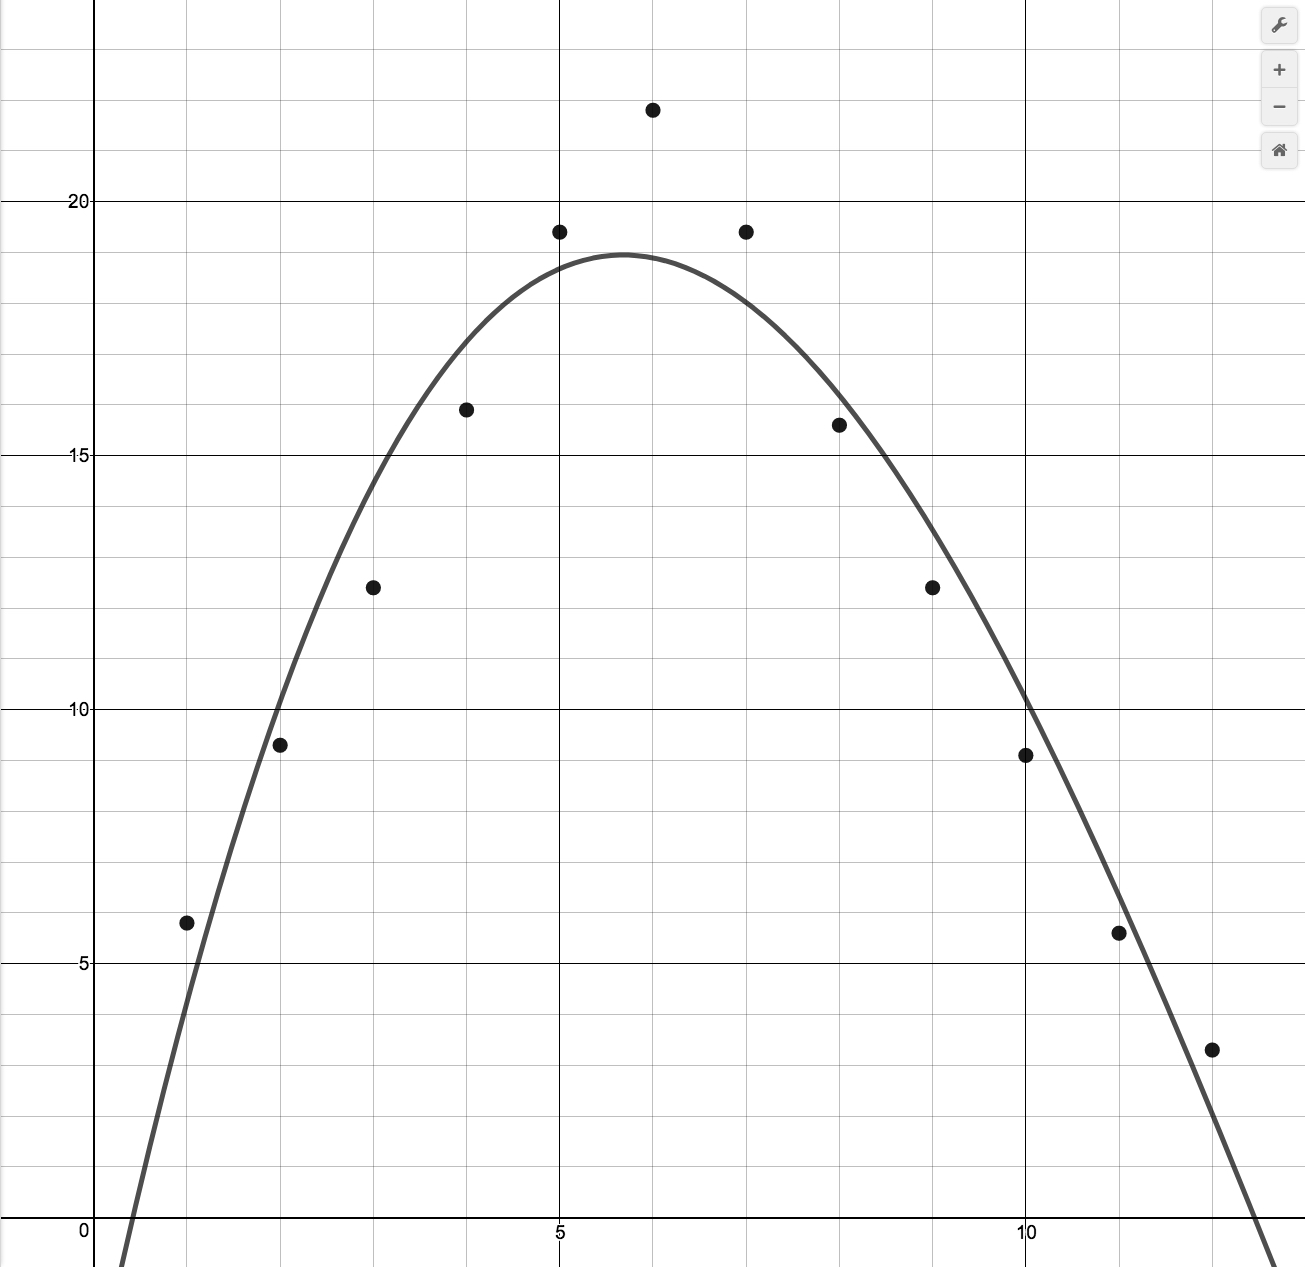
\includegraphics[width=2.5in]{./GraphsofPolynomialsGraphics/DaylightRegCubic.jpg} \hspace{.25in} & 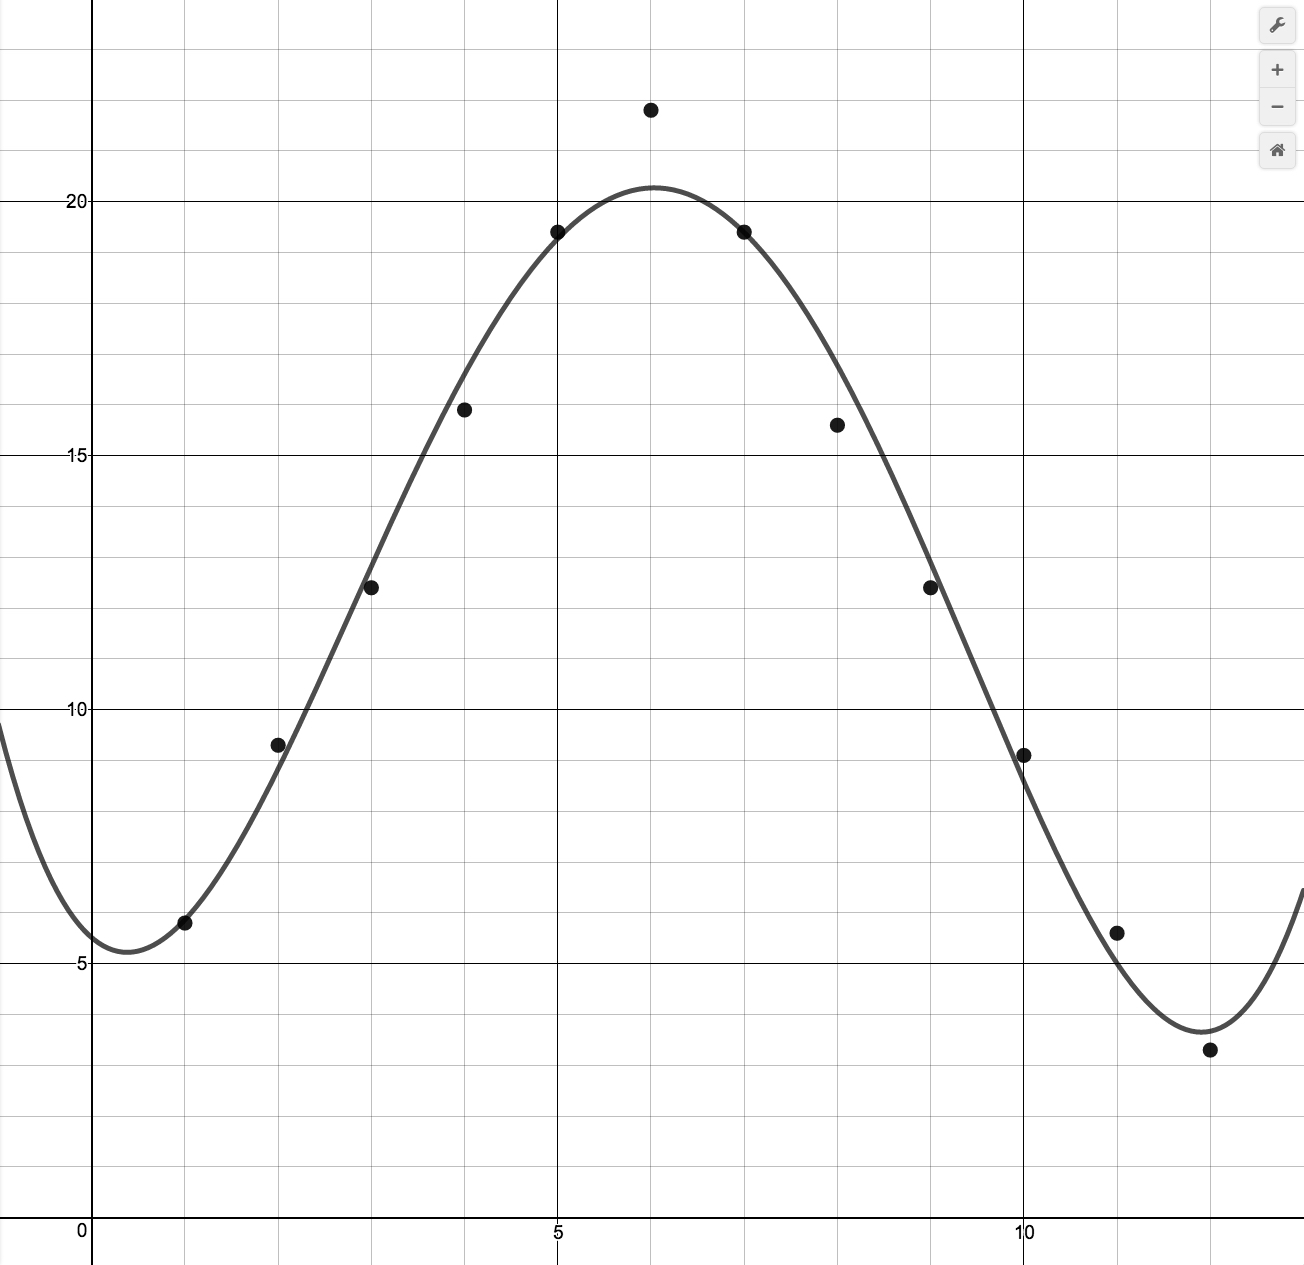
\includegraphics[width=2.5in]{./GraphsofPolynomialsGraphics/DaylightRegQuartic.jpg} \\

$y = p_{\mbox{\tiny $3$}}(x)$ \hspace{.25in} & $y = p_{\mbox{\tiny $4$}}(x)$ \\

\end{tabular}

\end{center}

\newpage

\item \begin{enumerate}

\item The scatter plot is shown below with each of the three regression models.

\item The quadratic model is $P_{\mbox{\tiny $2$}}(x) = -0.021x^{2} + 0.241x + 0.956$, $R^{2} = 0.7771$. \\
The cubic model is $P_{\mbox{\tiny $3$}}(x) = 0.005x^{3} - 0.103x^{2} + 0.602x + 0.573$,  $R^{2} = 0.9815$. \\
The quartic model is $P_{\mbox{\tiny $4$}}(x) = -0.000969x^{4} + 0.0253x^{3} - 0.240x^{2} + 0.944x + 0.330$,  $R^{2} = 0.9993$.

\item The models give maximums: $P_{\mbox{\tiny $2$}}(5.737) \approx 1.648$, $P_{\mbox{\tiny $3$}}(4.232) \approx 1.657$ and $P_{\mbox{\tiny $4$}}(3.784) \approx 1.630$.
\end{enumerate}



\hspace{-.1in} \begin{tabular}{ccc}

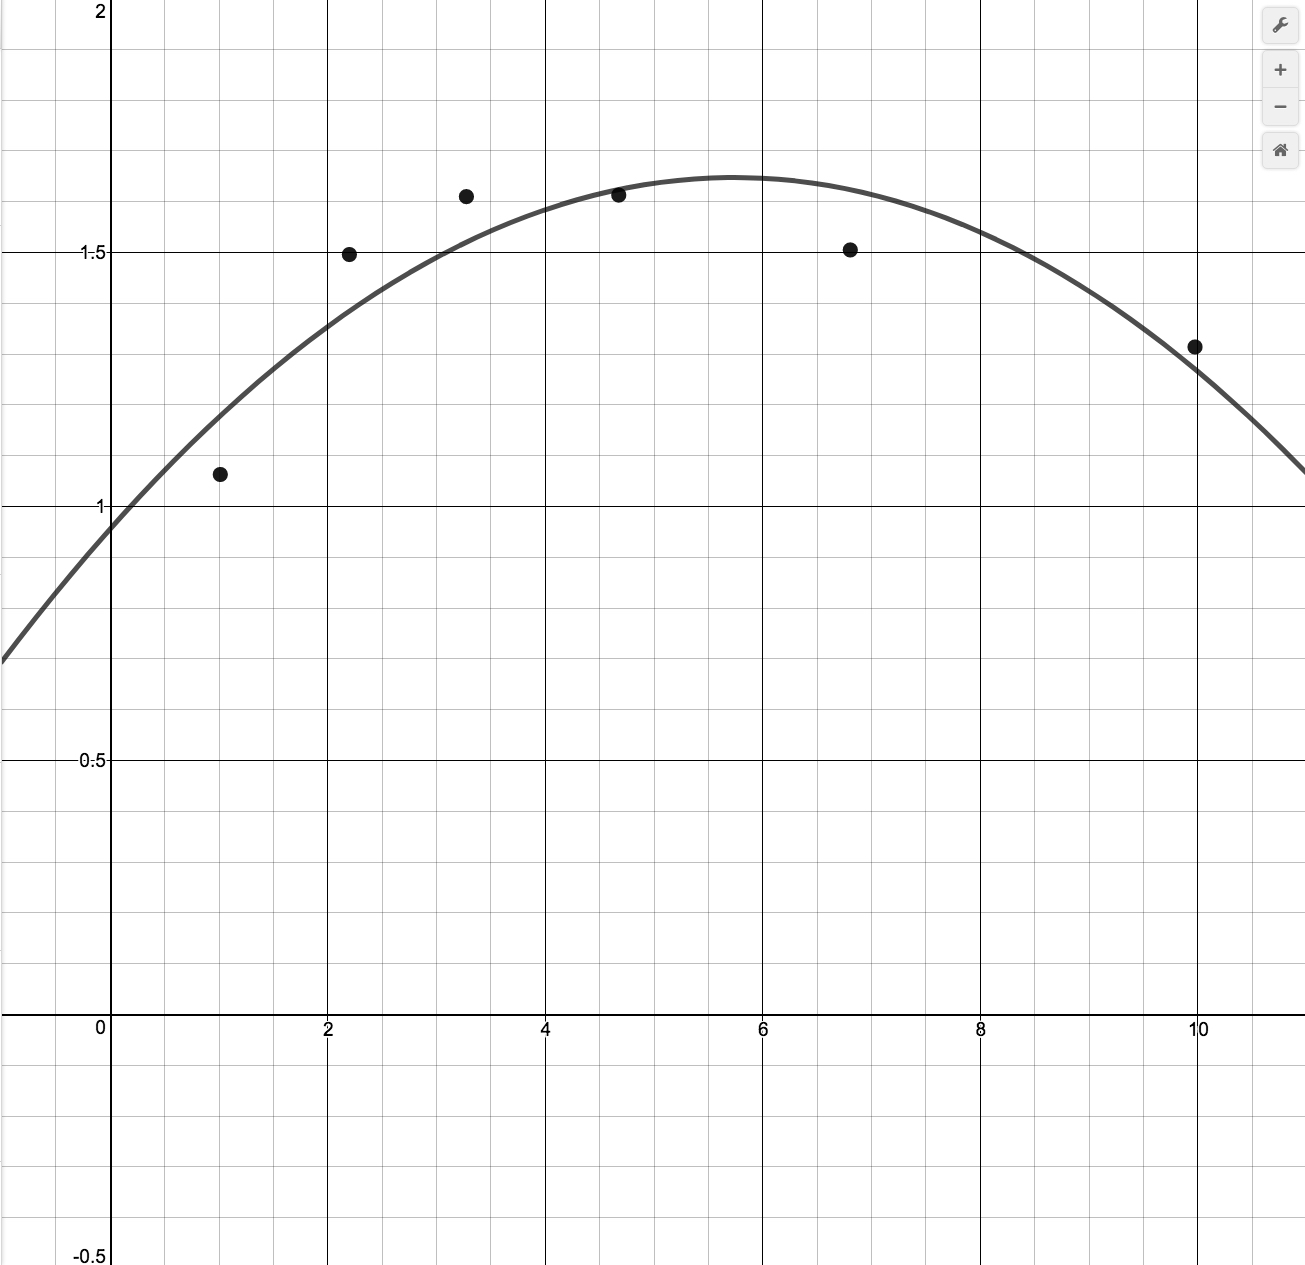
\includegraphics[width=1.8in]{./GraphsofPolynomialsGraphics/CircuitRegQuadratic.jpg} \hspace{.1in} &
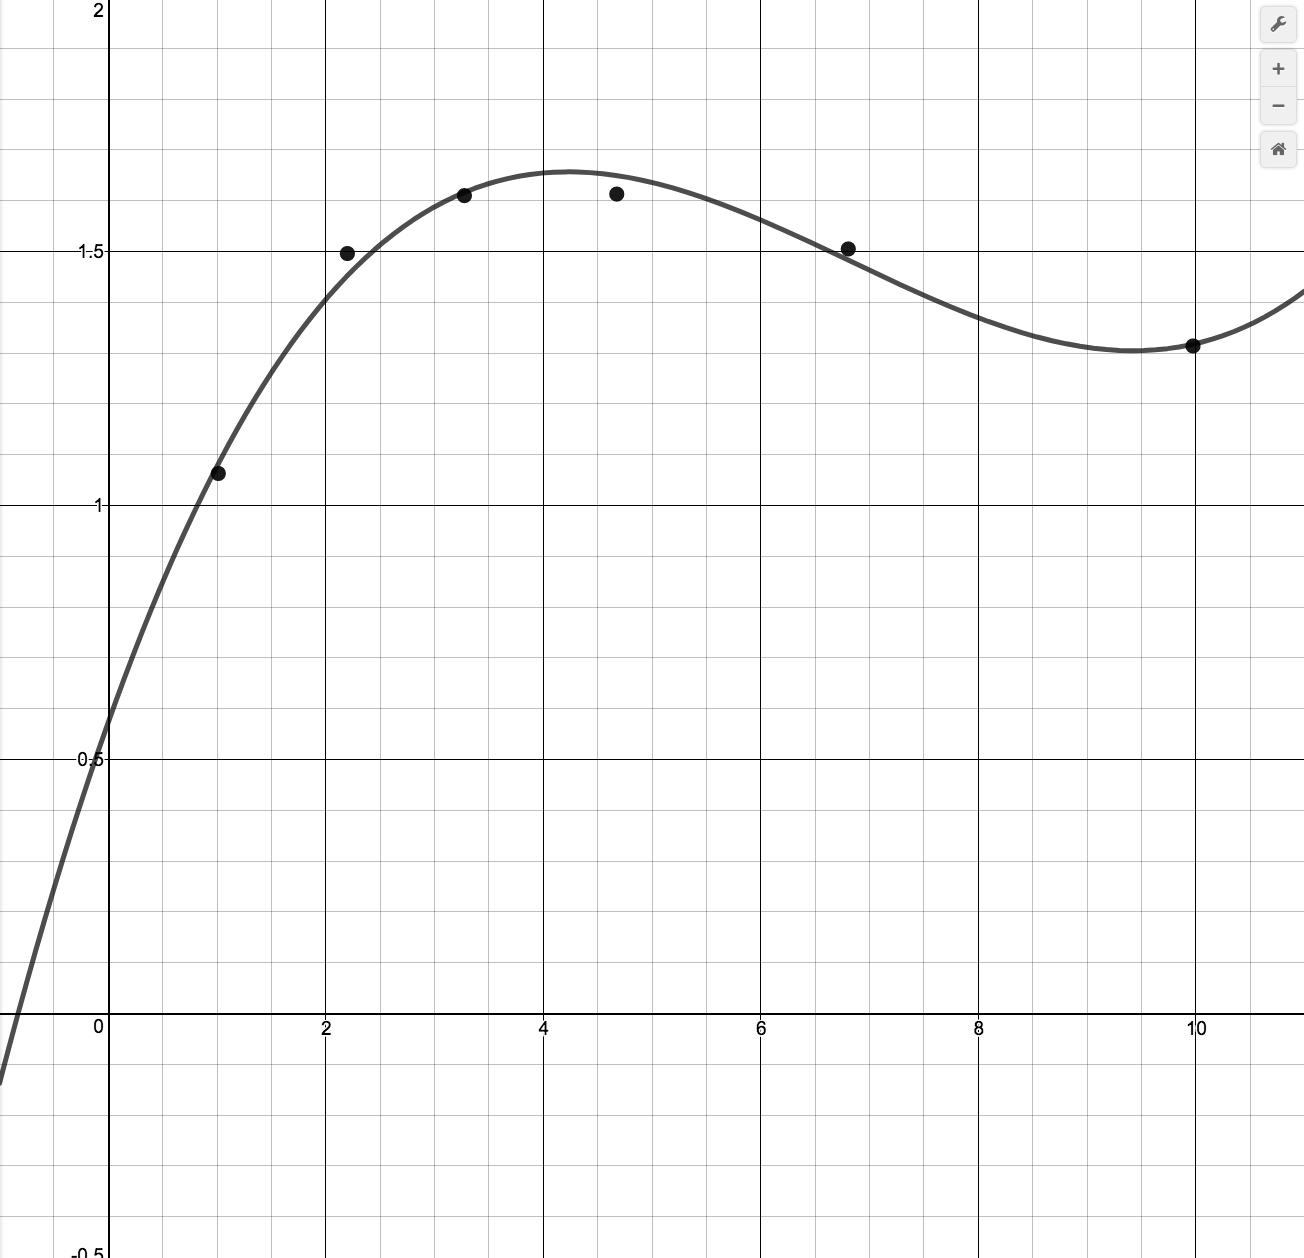
\includegraphics[width=1.8in]{./GraphsofPolynomialsGraphics/CircuitRegCubic.jpg} \hspace{.1in} &
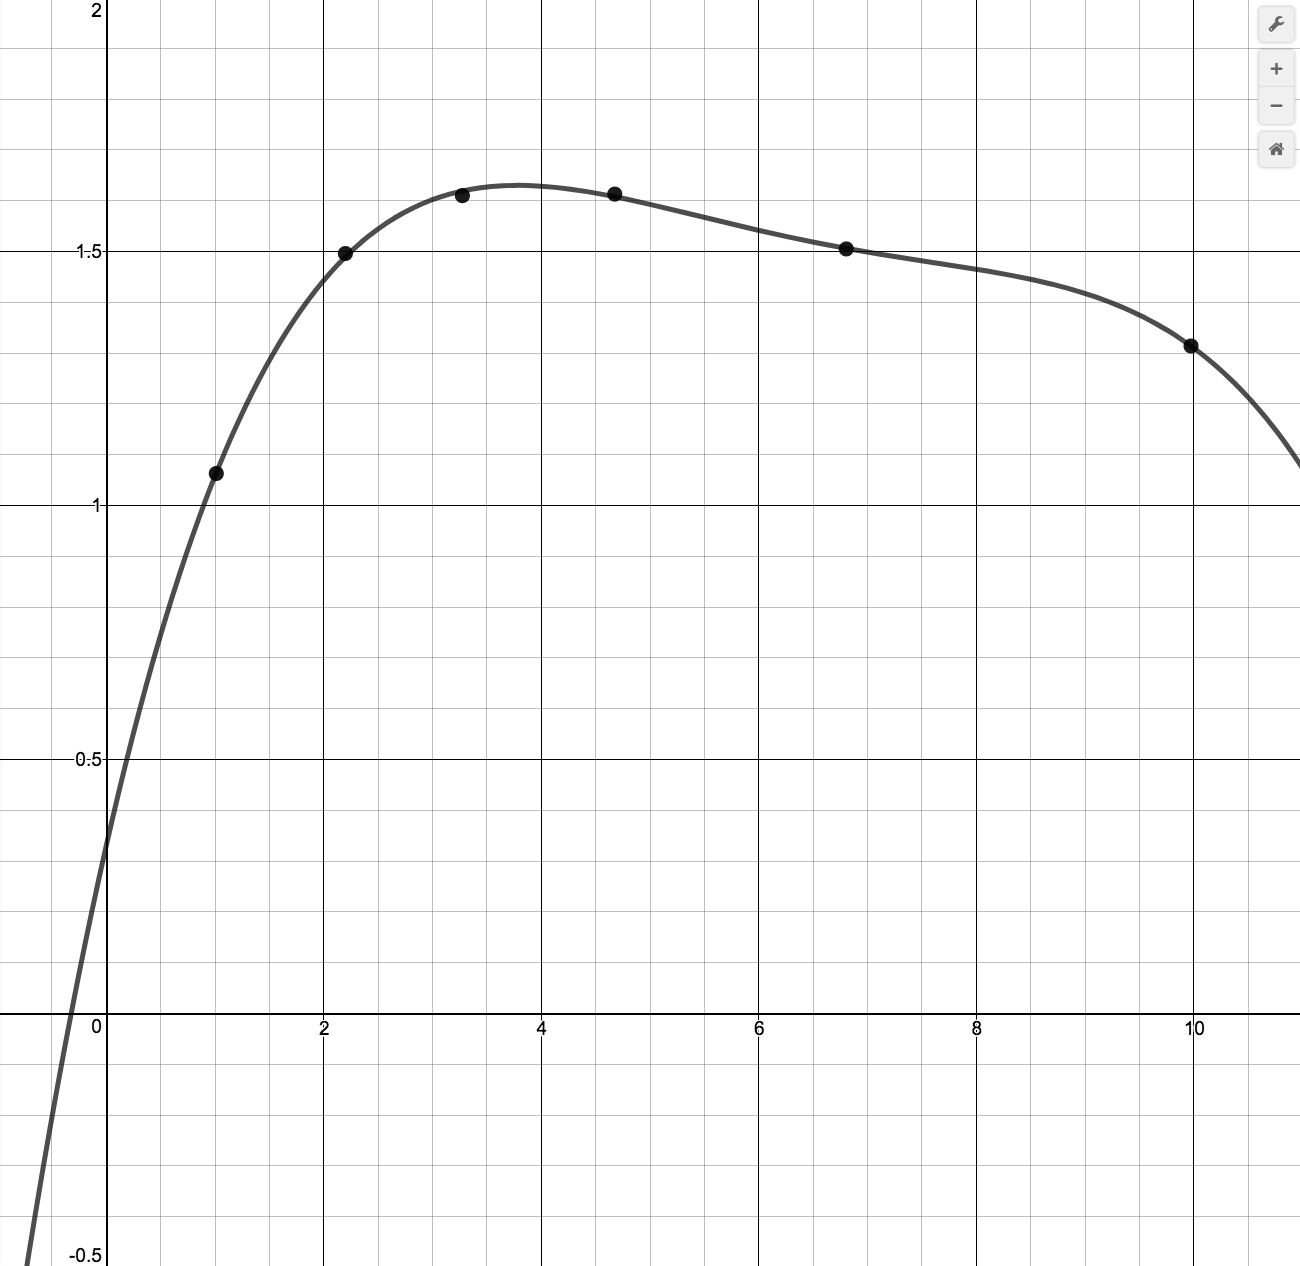
\includegraphics[width=1.8in]{./GraphsofPolynomialsGraphics/CircuitRegQuartic.jpg} \\

$y = P_{\mbox{\tiny $2$}}(x)$ \hspace{.1in} & $y = P_{\mbox{\tiny $3$}}(x)$ & $y = P_{\mbox{\tiny $4$}}(x)$\\

\end{tabular}

\item \begin{enumerate}

\item  as $x \rightarrow -\infty$, $p(x) \rightarrow -\infty$ and as $x \rightarrow \infty$, $p(x) \rightarrow -\infty$

\item The zeros appear to be: $x=-1.5$, even multiplicity - probably $2$ since it doesn't `look like' the graph is very flat near $x = 2$;  $x=0$, odd multiplicity - probably $1$ since the graph seems fairly linear as it passes through the origin;  $x=1$ odd multiplicity - probably $3$ or higher since the graph seems fairly `flat' near $x = 1$.

\item  local minimum:  approximately $(-0.773, -2.888)$;  local maximums:  approximately $(-1.5,0)$, and $(0.32, 0.532)$

\item  Based on the graph, even degree (at least $6$ based on multiplicities) with a negative leading coefficient based on the end behavior.

\item  We only have a \textit{portion} of the graph represented here.

\end{enumerate}

\addtocounter{enumi}{1}

\item We are looking for the largest open interval containing $x = -0.235$ for which the graph of $y = p(x)$ is at or above $y=-1.121$.  Since each of the gridlines on the $x$-axis correspond to $0.2$ units, we approximate this interval as  $(-1.25 \, \text{ish}, 1.1 \, \text{ish})$.

\addtocounter{enumi}{4}

\item 

\begin{multicols}{2}
\begin{enumerate} \addtocounter{enumii}{2} 
\item $L(x) = x^2$


\item $L(x) = x+1$

\end{enumerate}
\end{multicols}

\end{enumerate}


\closegraphsfile